% Combined TeX source bundle
% Title: Qin Jiushao, Shuxue Jiuzhang, current English bilingual fascicles 1-9
% Note: constituent files are preserved below in sources/. Some are standalone
% documents with their own preambles; this combined file is for inspection,
% comparison, and reuse rather than guaranteed one-command compilation.


% ============================================================
% Source: translations/en/chinese/qin-jiushao-shuxue-jiuzhang-fascicle1_bilingual.tex
% ============================================================

\documentclass[10pt,a4paper]{article}
\usepackage{fontspec}
\usepackage{amsmath,amssymb}
\usepackage{geometry}
\usepackage{xcolor}
\usepackage{fancyhdr}
\usepackage{enumitem}
\usepackage{hyperref}

\geometry{paperwidth=210mm,paperheight=297mm,left=12mm,right=12mm,top=20mm,bottom=20mm,headheight=14pt,footskip=28pt}

\setmainfont{Noto Sans CJK SC}
\setsansfont{Noto Sans CJK SC}

\tolerance=3000
\emergencystretch=3em
\hbadness=10000
\sloppy

\definecolor{titlecolor}{RGB}{45,55,72}
\definecolor{sectioncolor}{RGB}{55,65,81}
\definecolor{notecolor}{RGB}{120,53,15}
\definecolor{rulecolor}{RGB}{180,160,140}
\definecolor{prefacecolor}{RGB}{80,60,40}
\definecolor{labelcolor}{RGB}{90,60,30}

\makeatletter
\renewcommand{\section}{\@startsection{section}{1}{0mm}{1.2ex plus 0.3ex minus 0.1ex}{0.5ex plus 0.1ex}{\normalfont\large\bfseries\color{sectioncolor}}}
\renewcommand{\subsection}{\@startsection{subsection}{2}{0mm}{0.8ex plus 0.2ex minus 0.1ex}{0.3ex plus 0.1ex}{\normalfont\normalsize\bfseries\color{sectioncolor}}}
\makeatother

\pagestyle{fancy}
\fancyhf{}
\fancyhead[L]{\small\textit{Qin Jiushao -- Shuxue Jiuzhang -- Bilingual Edition}}
\fancyhead[R]{\small\thepage}
\renewcommand{\headrulewidth}{0.3pt}

\newcommand{\cnlabel}[1]{\textcolor{labelcolor}{\textbf{#1}}}
\newcommand{\enlabel}[1]{\textcolor{labelcolor}{\textbf{#1}}}
\newcommand{\transnote}[1]{\footnote{\textit{Trans.\ note:} #1}}

\newenvironment{problemsection}{%
  \medskip\par\noindent\textcolor{rulecolor}{\rule{\textwidth}{0.4pt}}\par\smallskip%
}{\par\smallskip\noindent\textcolor{rulecolor}{\rule{\textwidth}{0.4pt}}\par\medskip}

\newenvironment{prefacecn}{\begin{quote}\color{prefacecolor}\small}{\end{quote}}
\newenvironment{prefaceen}{\begin{quote}\color{prefacecolor}\small}{\end{quote}}

\hypersetup{colorlinks=true,linkcolor=sectioncolor,citecolor=sectioncolor,urlcolor=sectioncolor,pdfencoding=auto}

\begin{document}

\begin{titlepage}
\centering
\vspace*{2.5cm}
{\fontsize{22}{28}\selectfont\textcolor{titlecolor}{数书九章}}
\vspace{0.5cm}

{\fontsize{12}{15}\selectfont\textcolor{sectioncolor}{\textit{Mathematical Treatise in Nine Sections}}}
\vspace{0.8cm}

{\Large\bfseries Fascicle I -- The Dayan Category}
\vspace{0.3cm}

{\large Bilingual Edition / 双语版}
\vspace{1.5cm}

{\large By \textbf{Qin Jiushao} (秦九韶)\\[0.3em] c.\ 1202--1261 CE\\[0.3em] \textit{Presented in the 7th year of Chunyou (淳祐七年), 1247 CE}}
\vspace{1.2cm}

\begin{minipage}{0.85\textwidth}
\centering
\textit{Left side: Original Classical Chinese text\\ Right side: English translation with modern mathematical commentary}
\end{minipage}
\vfill
{\small Typeset in \LaTeX\ with XeTeX --- Bilingual Edition}
\end{titlepage}

\tableofcontents
\newpage

%% ========================================================================
\section{Introduction / 导言}

\noindent\begin{minipage}[t]{0.47\textwidth}
\begin{flushleft}
\textbf{\large 数书九章序}
\end{flushleft}
\end{minipage}%
\hfill\vrule width 0.3pt\hfill%
\begin{minipage}[t]{0.47\textwidth}
\begin{flushleft}
\textbf{\large Preface to the Shuxue Jiuzhang}
\end{flushleft}
\end{minipage}

\vspace{0.5em}

\noindent\begin{minipage}[t]{0.47\textwidth}
\begin{flushleft}
\small
数书九章者，南宋秦九韶之所著也。秦氏字道古，鲁郡人。生于宋季，博学多能，尤精算学。此书成于淳祐七年（公元1247年），凡九卷，每卷九问，共八十一题。其学大衍、天时、田域、测望、赋役、钱谷、营建、军旅、市易九类。
\end{flushleft}
\end{minipage}%
\hfill\vrule width 0.3pt\hfill%
\begin{minipage}[t]{0.47\textwidth}
\begin{flushleft}
\small
The \textit{Shuxue Jiuzhang} (Mathematical Treatise in Nine Sections) is the magnum opus of the Song dynasty mathematician Qin Jiushao (秦九韶, c.~1202--1261). Completed in 1247 CE during the Chunyou era (淳祐七年), it stands as one of the greatest achievements in the history of Chinese mathematics and indeed of world mathematics.
\end{flushleft}
\end{minipage}

\vspace{0.5em}

\noindent\begin{minipage}[t]{0.47\textwidth}
\begin{flushleft}
\small
每问有问、答、术、草四目，体例谨严。大衍之类，尤推精妙，盖中国剩余定理之滥觞也。
\end{flushleft}
\end{minipage}%
\hfill\vrule width 0.3pt\hfill%
\begin{minipage}[t]{0.47\textwidth}
\begin{flushleft}
\small
The work is organized into nine categories (类), each containing nine problems (问), for a total of eighty-one problems. Each problem follows a rigorous four-part structure: \textbf{Wen} (问) -- the problem statement; \textbf{Da} (答) -- the numerical answer; \textbf{Shu} (术) -- the general method; \textbf{Cao} (草) -- the detailed working.
\end{flushleft}
\end{minipage}

\subsection{The Nine Categories / 九类名目}

\noindent\begin{minipage}[t]{0.47\textwidth}
\begin{flushleft}
\small
九类之目：
\begin{enumerate}[label=\arabic*.,leftmargin=*,nosep,topsep=2pt]
  \item \textbf{大衍} -- 求一之术
  \item \textbf{天时} -- 天文历法
  \item \textbf{田域} -- 田地测量
  \item \textbf{测望} -- 勾股重差
  \item \textbf{赋役} -- 租税劳役
  \item \textbf{钱谷} -- 钱粮贸易
  \item \textbf{营建} -- 建筑工事
  \item \textbf{军旅} -- 兵家之事
  \item \textbf{市易} -- 市场交易
\end{enumerate}
\end{flushleft}
\end{minipage}%
\hfill\vrule width 0.3pt\hfill%
\begin{minipage}[t]{0.47\textwidth}
\begin{flushleft}
\small
The nine categories are:
\begin{enumerate}[label=\arabic*.,leftmargin=*,nosep,topsep=2pt]
  \item \textbf{Dayan} (大衍) -- ``Great Derivation'': Indeterminate analysis and the Chinese Remainder Theorem
  \item \textbf{Tianshi} (天时) -- Astronomical phenomena and calendar calculations
  \item \textbf{Tianyu} (田域) -- Land measurement and area calculation
  \item \textbf{Cewang} (测望) -- Surveying and observation
  \item \textbf{Fuyi} (赋役) -- Taxation and labor service
  \item \textbf{Qian'gu} (钱谷) -- Currency and grain commerce
  \item \textbf{Yingjian} (营建) -- Construction and engineering
  \item \textbf{Junlv} (军旅) -- Military affairs
  \item \textbf{Shiyi} (市易) -- Market transactions
\end{enumerate}
\end{flushleft}
\end{minipage}

\newpage

%% ========================================================================
\section{Preface / 序}

\noindent\begin{minipage}[t]{0.47\textwidth}
\begin{flushleft}
\begin{prefacecn}
周教六艺，数实成之。学士大夫所从事尚矣。其用本太虚生一，而周流无穷。大则可以通神明、顺性命，小则可以经世务、类万物，讵容以浅近窥哉？
\end{prefacecn}
\end{flushleft}
\end{minipage}%
\hfill\vrule width 0.3pt\hfill%
\begin{minipage}[t]{0.47\textwidth}
\begin{flushleft}
\begin{prefaceen}
Of the Six Arts taught by the Zhou, mathematics completes them. It has long been pursued by scholars and gentlemen. Its use originates from the One born of the Great Void, flowing endlessly. In the large, it can penetrate the divine and accord with nature; in the small, it can govern worldly affairs and classify all things. How could it be viewed as shallow or trivial?
\end{prefaceen}
\end{flushleft}
\end{minipage}

\vspace{0.3em}

\noindent\begin{minipage}[t]{0.47\textwidth}
\begin{flushleft}
\begin{prefacecn}
若昔推策以迎日，定律而和气。髀距濬川，土圭度晷。天地之大，囿焉而不能外，况其间总总者乎？爰自河图洛书，闿发幽秘；八卦九畴，错综精微。
\end{prefacecn}
\end{flushleft}
\end{minipage}%
\hfill\vrule width 0.3pt\hfill%
\begin{minipage}[t]{0.47\textwidth}
\begin{flushleft}
\begin{prefaceen}
From ancient times, reckoning rods were used to predict the sun's course, and laws were established to harmonize the qi. The gnomon measured the rivers, the jade tablet measured the shadows. The greatness of heaven and earth is encompassed by it and cannot escape, how much more the multitude of things within?
\end{prefaceen}
\end{flushleft}
\end{minipage}

\vspace{0.3em}

\noindent\begin{minipage}[t]{0.47\textwidth}
\begin{flushleft}
\begin{prefacecn}
极而至于大衍、皇极之用，而人事之变无不该，鬼神之情莫能隐矣。圣人神之言而遗其粗，常人昧之由而莫之觉。要其归，则数与道非二本也。
\end{prefacecn}
\end{flushleft}
\end{minipage}%
\hfill\vrule width 0.3pt\hfill%
\begin{minipage}[t]{0.47\textwidth}
\begin{flushleft}
\begin{prefaceen}
Reaching to the applications of the Dayan and the Supreme Ultimate, there is no human affair that it does not encompass, no spirit's nature that it cannot reveal. The sages found its spirit and left its roughness; ordinary people are blind to its path. In essence, number and the Way are not two different roots.
\end{prefaceen}
\end{flushleft}
\end{minipage}

\vspace{0.3em}

\noindent\begin{minipage}[t]{0.47\textwidth}
\begin{flushleft}
\begin{prefacecn}
独大衍法不载九章，未有能推之者。历家演法颇用之，以为方程者，误也。
\end{prefacecn}
\end{flushleft}
\end{minipage}%
\hfill\vrule width 0.3pt\hfill%
\begin{minipage}[t]{0.47\textwidth}
\begin{flushleft}
\begin{prefaceen}
Only the Dayan method is not recorded in the Nine Chapters, and none have been able to develop it. Calendarists have used it extensively in their computational methods, but those who take it as a system of equations are mistaken.
\end{prefaceen}
\end{flushleft}
\end{minipage}

\vspace{0.3em}

\noindent\begin{minipage}[t]{0.47\textwidth}
\begin{flushleft}
\begin{prefacecn}
九韶愚陋，不闲于艺。然早岁侍亲中都，因得访习于太史，又尝从隐君子受数学。时际兵难，历岁遥塞，不自意全于矢石之间。更险离忧，荏苒十禩，心槁气落。信知夫物莫不有数也，乃肆意其间，旁诹方能，探索杳眇，粗若有得焉。
\end{prefacecn}
\end{flushleft}
\end{minipage}%
\hfill\vrule width 0.3pt\hfill%
\begin{minipage}[t]{0.47\textwidth}
\begin{flushleft}
\begin{prefaceen}
I, Jiushao, am foolish and unrefined, not skilled in the arts. Yet in my youth I served my parents in the capital, and so had the opportunity to study with the Grand Astrologer; I also received instruction in mathematics from a gentleman recluse. When the time of military disaster came, I did not expect to survive between arrows and stones. Passing through danger and sorrow, ten years elapsed; my heart withered and my spirit fell. Truly I came to know that all things have number.
\end{prefaceen}
\end{flushleft}
\end{minipage}

\vspace{0.3em}

\noindent\begin{minipage}[t]{0.47\textwidth}
\begin{flushleft}
\begin{prefacecn}
时淳祐七年九月，鲁郡秦九韶叙。
\end{prefacecn}
\end{flushleft}
\end{minipage}%
\hfill\vrule width 0.3pt\hfill%
\begin{minipage}[t]{0.47\textwidth}
\begin{flushleft}
\begin{prefaceen}
Written in the ninth month of the seventh year of Chunyou, by Qin Jiushao of Lu Commandery.
\end{prefaceen}
\end{flushleft}
\end{minipage}

\newpage

%% ========================================================================
\section{The Dayan General Method / 大衍总数术}

\subsection{Editor's Commentary / 按语}

\noindent\begin{minipage}[t]{0.47\textwidth}
\begin{flushleft}
\begin{prefacecn}
按大衍术，以各分数之奇零求各分数之总数。大而天行，小而物数，皆可御之。其法有求元、求定、求衍、求奇、求乘、求用之目。大约以数之奇偶为根，而以诸数相度之尽不尽为用。
\end{prefacecn}
\end{flushleft}
\end{minipage}%
\hfill\vrule width 0.3pt\hfill%
\begin{minipage}[t]{0.47\textwidth}
\begin{flushleft}
\begin{prefaceen}
\textit{Editor's note:} The Dayan method takes the remainders (odd fragments) of each fractional divisor to find the total number. Whether for large celestial motions or small material quantities, it can be applied. The method has the following steps: finding the original numbers, finding the definitive numbers, finding the derivative numbers, finding the odd numbers, finding the multipliers, and finding the use numbers.
\end{prefaceen}
\end{flushleft}
\end{minipage}

\subsection{The Four Types of Numbers / 四种问数}

\noindent\begin{minipage}[t]{0.47\textwidth}
\begin{flushleft}
\small
\cnlabel{大衍总数术曰：}置诸问数，类名有四。

\begin{enumerate}[label=\arabic*.,leftmargin=*,nosep,topsep=2pt]
  \item \textbf{元数} -- 谓尾位见单零者
  \item \textbf{收数} -- 谓尾位见分厘者
  \item \textbf{通数} -- 谓诸数各有分子分母者
  \item \textbf{复数} -- 谓尾位见十或百及千以上者
\end{enumerate}
\end{flushleft}
\end{minipage}%
\hfill\vrule width 0.3pt\hfill%
\begin{minipage}[t]{0.47\textwidth}
\begin{flushleft}
\small
\enlabel{The Dayan General Method states:} Place the given numbers; there are four types.

\begin{enumerate}[label=\arabic*.,leftmargin=*,nosep,topsep=2pt]
  \item \textbf{Original numbers} -- Numbers ending in single units
  \item \textbf{Collected numbers} -- Numbers ending in fractional parts
  \item \textbf{Common numbers} -- Numbers each having numerator and denominator
  \item \textbf{Repeated numbers} -- Numbers ending in tens, hundreds, or thousands
\end{enumerate}
\end{flushleft}
\end{minipage}

\subsection{Finding the Definitive Numbers / 求定数}

\noindent\begin{minipage}[t]{0.47\textwidth}
\begin{flushleft}
\small
\cnlabel{元数者：}先以两两连环求等，约奇弗约偶。或约得五而彼有十，乃约偶弗约奇。或元数俱偶，约毕可存一位见偶。
\end{flushleft}
\end{minipage}%
\hfill\vrule width 0.3pt\hfill%
\begin{minipage}[t]{0.47\textwidth}
\begin{flushleft}
\small
\enlabel{For original numbers:} First, pairwise in chain sequence find the GCD; reduce the odd one, not the even one. If reducing yields 5 while the other has 10, then reduce the even one, not the odd one. If all original numbers are even, after reduction one may keep one even number.
\end{flushleft}
\end{minipage}

\vspace{0.3em}

\noindent\begin{minipage}[t]{0.47\textwidth}
\begin{flushleft}
\small
\cnlabel{复数者：}问数尾位见十以上者，以诸数求总等，存一位约众位，始得元数。两两连环求等，约奇弗约偶，复乘偶；或约偶弗约奇，弗乘奇。
\end{flushleft}
\end{minipage}%
\hfill\vrule width 0.3pt\hfill%
\begin{minipage}[t]{0.47\textwidth}
\begin{flushleft}
\small
\enlabel{For repeated numbers:} When the given numbers end in ten or above, find the total GCD of all numbers; keep one position and reduce the rest. Then pairwise in chain sequence find GCDs; reduce the odd, not the even, and multiply back the even; or reduce the even, not the odd, and do not multiply back the odd.
\end{flushleft}
\end{minipage}

\subsection{Computing the Derivative Numbers / 求衍数}

\noindent\begin{minipage}[t]{0.47\textwidth}
\begin{flushleft}
\small
\cnlabel{求定数}勿使两位见偶，勿使见一太多。见一多则借用繁，不欲借则任得一。

\cnlabel{以定相乘为衍母}，以各定约衍母，得各衍数。

次以各定母满去衍数，各余名曰\cnlabel{奇数}。

以\cnlabel{大衍求一术}，得各\cnlabel{乘率}。

以乘衍数，各得\cnlabel{用数}。
\end{flushleft}
\end{minipage}%
\hfill\vrule width 0.3pt\hfill%
\begin{minipage}[t]{0.47\textwidth}
\begin{flushleft}
\small
\enlabel{Finding definitive numbers:} Do not let two positions be even; do not let there be too many ones. Too many ones makes borrowing complicated.

\enlabel{Multiply the definitive numbers together to obtain the derivative mother.} Reduce the derivative mother by each definitive number to obtain each \enlabel{derivative number}.

Next, reduce each derivative number by its corresponding definitive number; the remainders are called the \enlabel{odd numbers}.

Using the \enlabel{Dayan Method for Finding Unity}, obtain each \enlabel{multiplier}.

Multiplying each multiplier by its derivative number gives each \enlabel{use number}.
\end{flushleft}
\end{minipage}

\vspace{0.5em}

\noindent\textcolor{rulecolor}{\rule{\textwidth}{0.4pt}}

\subsection{The Dayan Method for Finding Unity / 大衍求一术}

\noindent\begin{minipage}[t]{0.47\textwidth}
\begin{flushleft}
\begin{prefacecn}
大衍求一术云：置奇右上，定居右下。立天元一于左上。先以右行上下两位，以少除多，所得商数，乃递互乘归左行。须使右上末后奇一而止。乃验左上所得，以为乘率。或奇数已见单一者，便为乘率。
\end{prefacecn}
\end{flushleft}
\end{minipage}%
\hfill\vrule width 0.3pt\hfill%
\begin{minipage}[t]{0.47\textwidth}
\begin{flushleft}
\begin{prefaceen}
The Dayan Method for Finding Unity says: Place the odd number at the upper right, the definitive number at the lower right. Place the celestial element unity (1) at the upper left. First, divide the larger by the smaller of the two numbers in the right column; the quotient obtained is then used to multiply alternately into the left column. Continue until the upper right finally becomes one. Then check what is obtained at the upper left---this is the multiplier.
\end{prefaceen}
\end{flushleft}
\end{minipage}

\vspace{0.5em}

\textit{In modern mathematical terms:} Given coprime integers $a$ (the ``odd number'') and $m$ (the ``definitive number''), find $k$ such that:
\[k \cdot a \equiv 1 \pmod{m}\]
This is the \textbf{modular multiplicative inverse} of $a$ modulo $m$, computed by the \textbf{extended Euclidean algorithm}.

\newpage

%% ========================================================================
\section{Problem 1: Shigua Fawei / 蓍卦发微}

\begin{problemsection}

\noindent\begin{minipage}[t]{\textwidth}
\begin{center}
\textbf{蓍卦发微} -- \textbf{Divination by Yarrow Stalks}
\end{center}
\end{minipage}

\vspace{0.3em}

\noindent\begin{minipage}[t]{0.47\textwidth}
\begin{flushleft}
\small
\cnlabel{问曰：}

《易》曰：大衍之数五十，其用四十有九。又曰：分而为二以象两，挂一以象三，揲之以四以象四时。三变而成爻，十有八变而成卦。欲知所衍之术及其数各几何？
\end{flushleft}
\end{minipage}%
\hfill\vrule width 0.3pt\hfill%
\begin{minipage}[t]{0.47\textwidth}
\begin{flushleft}
\small
\enlabel{Question:}

The \textit{Book of Changes} says: ``The number of the Great Derivation is fifty; of these, forty-nine are used.'' It also says: ``Divide into two to symbolize the Two [heaven and earth]; hang one to symbolize the Three [heaven, earth, and man]; count off by fours to symbolize the Four Seasons.'' Three changes produce a line; eighteen changes produce a hexagram. The problem asks to find the computational method of this derivation and the numbers involved.

\textit{This problem applies the Dayan method to the classical yarrow-stalk divination of the I Ching.}
\end{flushleft}
\end{minipage}

\vspace{0.3em}

\noindent\begin{minipage}[t]{0.47\textwidth}
\begin{flushleft}
\small
\cnlabel{答曰：}

衍母十二，衍法三。

一元衍数二十四，二元衍数一十二，三元衍数八，四元衍数六。以上四位衍数，计五十一。

一揲用数一十二，二揲用数二十四，三揲用数四，四揲用数九。以上四位用数，计四十九。
\end{flushleft}
\end{minipage}%
\hfill\vrule width 0.3pt\hfill%
\begin{minipage}[t]{0.47\textwidth}
\begin{flushleft}
\small
\enlabel{Answer:}

The derivative mother is 12, the derivative divisor is 3.

The first derivative number is 24, the second is 12, the third is 8, the fourth is 6. The sum of these four derivative numbers is 51.

The first manipulation use-number is 12, the second is 24, the third is 4, the fourth is 9. The sum of these four use-numbers is 49.\transnote{The sum 49 corresponds to ``the number of the Great Derivation is fifty, of which forty-nine are used'' from the \textit{Yijing}.}
\end{flushleft}
\end{minipage}

\vspace{0.3em}

\noindent\begin{minipage}[t]{0.47\textwidth}
\begin{flushleft}
\small
\cnlabel{术曰：}

置诸元数，两两连环求等，约奇弗约偶。遍约毕，乃变元数皆曰定母，列右行。各立天元一为子，列左行。以诸定母互乘左行之子，各得名曰衍数。
\end{flushleft}
\end{minipage}%
\hfill\vrule width 0.3pt\hfill%
\begin{minipage}[t]{0.47\textwidth}
\begin{flushleft}
\small
\enlabel{Method:}

Place the given original numbers; pairwise in chain sequence find the GCD, reducing the odd and not the even. When reduction is complete everywhere, the original numbers become the definitive numbers; place them in the right column. Place the celestial element unity (1) as the seed in the left column. Cross-multiply the definitive numbers with the seeds in the left column; each result is called a derivative number.
\end{flushleft}
\end{minipage}

\vspace{0.3em}

\noindent\begin{minipage}[t]{0.47\textwidth}
\begin{flushleft}
\small
次以各定母满去衍数，各余名曰奇数。以奇数与定母用大衍术求一，得各乘率。以乘衍数，各得用数。
\end{flushleft}
\end{minipage}%
\hfill\vrule width 0.3pt\hfill%
\begin{minipage}[t]{0.47\textwidth}
\begin{flushleft}
\small
Next, reduce each derivative number by its corresponding definitive number; each remainder is called the odd number. Using the Dayan Method for Finding Unity on the odd number and the definitive number, obtain each multiplier. Multiply each derivative number by its multiplier to obtain each use number.
\end{flushleft}
\end{minipage}

\end{problemsection}

\newpage

%% ========================================================================
\section{Problem 2: Guli Huiji / 古历会积}

\begin{problemsection}

\noindent\begin{minipage}[t]{\textwidth}
\begin{center}
\textbf{古历会积} -- \textbf{Ancient Calendar Accumulation}
\end{center}
\end{minipage}

\vspace{0.3em}

\noindent\begin{minipage}[t]{0.47\textwidth}
\begin{flushleft}
\small
\cnlabel{问曰：}

问古历会积，欲求积年。以历法积元为问，历过无考，但据近世演纪之法，推而上之。
\end{flushleft}
\end{minipage}%
\hfill\vrule width 0.3pt\hfill%
\begin{minipage}[t]{0.47\textwidth}
\begin{flushleft}
\small
\enlabel{Question:}

This problem concerns the calculation of the accumulated years (积年) in ancient calendar systems. Given certain astronomical periodicities, one must find a number that simultaneously satisfies multiple congruence conditions. The epochs have passed without record; based on the method of computing epochs used in recent times, one extrapolates backward.

\textit{This was one of the primary applications of the Dayan method in traditional Chinese astronomy---finding a common epoch that aligns multiple celestial cycles.}
\end{flushleft}
\end{minipage}

\vspace{0.3em}

\noindent\begin{minipage}[t]{0.47\textwidth}
\begin{flushleft}
\small
\cnlabel{术曰：}

以大衍求之。置元历相关诸周期，连环求等，约奇弗约偶，得定母。诸定相乘为衍母。以各定约衍母得衍数。各满定母去之，余为奇数。大衍求一入之，得乘率。以乘衍数为用数。次置各余数乘用数，并之为总数。满衍母去之，不满为所求积年。
\end{flushleft}
\end{minipage}%
\hfill\vrule width 0.3pt\hfill%
\begin{minipage}[t]{0.47\textwidth}
\begin{flushleft}
\small
\enlabel{Method:}

Solve by the Dayan method. Place the relevant periods of the original calendar; pairwise in chain sequence find GCDs, reducing the odd and not the even, obtaining the definitive numbers. Multiply the definitive numbers together to obtain the derivative mother. Reduce the derivative mother by each definitive number to obtain the derivative numbers. Reduce each by its definitive number; the remainders are the odd numbers. Apply the Dayan Method for Finding Unity to obtain the multipliers. Multiply the derivative numbers by the multipliers to obtain the use numbers. Next, place each remainder, multiply by the use numbers, and sum to obtain the total number. Reduce by the derivative mother; the remainder is the sought accumulated years.
\end{flushleft}
\end{minipage}

\end{problemsection}

\newpage

%% ========================================================================
\section{Problem 3: Tuiji Tugong / 推计土功}

\begin{problemsection}

\noindent\begin{minipage}[t]{\textwidth}
\begin{center}
\textbf{推计土功} -- \textbf{Estimating Earthworks}
\end{center}
\end{minipage}

\vspace{0.3em}

\noindent\begin{minipage}[t]{0.47\textwidth}
\begin{flushleft}
\small
\cnlabel{问曰：}

四县（甲、乙、丙、丁）共同筑堤，根据各县的物力分配筑堤任务。

\begin{itemize}[leftmargin=*,nosep,topsep=2pt]
  \item 甲县物力：138,600贯
  \item 乙县物力：146,300贯
  \item 丙县物力：192,500贯
  \item 丁县物力：184,800贯
\end{itemize}

筑堤标准：每770贯物力分配一名劳动力，每人每天筑堤60平方尺。

进度情况：甲县和乙县已完成任务，丙县剩余51丈，丁县剩余18丈。
\end{flushleft}
\end{minipage}%
\hfill\vrule width 0.3pt\hfill%
\begin{minipage}[t]{0.47\textwidth}
\begin{flushleft}
\small
\enlabel{Question:}

Four counties (A, B, C, D) jointly build a dike; the task is distributed according to each county's resources.

\begin{itemize}[leftmargin=*,nosep,topsep=2pt]
  \item County A resources: 138,600 guan
  \item County B resources: 146,300 guan
  \item County C resources: 192,500 guan
  \item County D resources: 184,800 guan
\end{itemize}

Dike standard: for every 770 guan of resources, assign one laborer; each laborer builds 60 square feet of dike per day.

Progress: Counties A and B have completed their tasks; County C has 51 zhang remaining; County D has 18 zhang remaining.

\textit{This is a classic indeterminate problem solved by the Dayan method.}
\end{flushleft}
\end{minipage}

\vspace{0.3em}

\noindent\begin{minipage}[t]{0.47\textwidth}
\begin{flushleft}
\small
\cnlabel{答曰：}

堤的总长度为19里235步5尺。

各县所筑长度：
\begin{itemize}[leftmargin=*,nosep,topsep=2pt]
  \item 甲县：1,260丈
  \item 乙县：1,768步5尺6寸
  \item 丙县：4里328步5尺6寸
  \item 丁县：与前三县相应
\end{itemize}
\end{flushleft}
\end{minipage}%
\hfill\vrule width 0.3pt\hfill%
\begin{minipage}[t]{0.47\textwidth}
\begin{flushleft}
\small
\enlabel{Answer:}

The total length of the dike is 19 li 235 bu 5 chi.

Each county's contribution:
\begin{itemize}[leftmargin=*,nosep,topsep=2pt]
  \item County A: 1,260 zhang
  \item County B: 1,768 bu 5 chi 6 cun
  \item County C: 4 li 328 bu 5 chi 6 cun
  \item County D: corresponding to the first three
\end{itemize}
\end{flushleft}
\end{minipage}

\vspace{0.3em}

\noindent\begin{minipage}[t]{0.47\textwidth}
\begin{flushleft}
\small
\cnlabel{术曰：}

以大衍求之。置各县物力，连环求等，约奇弗约偶，得定母。诸定相乘为衍母。以各定约衍母得衍数。各满定母去之，余为奇数。大衍求一入之，得乘率。以乘衍数为用数。次置各县余数乘用数，并之为总数。满衍母去之，不满为所求。
\end{flushleft}
\end{minipage}%
\hfill\vrule width 0.3pt\hfill%
\begin{minipage}[t]{0.47\textwidth}
\begin{flushleft}
\small
\enlabel{Method:}

Solve by the Dayan method. Place the resources of each county; pairwise in chain sequence find GCDs, reducing the odd and not the even, obtaining the definitive numbers. Multiply the definitive numbers together to obtain the derivative mother. Reduce the derivative mother by each definitive number to obtain the derivative numbers. Reduce each by its definitive number; the remainders are the odd numbers. Apply the Dayan Method for Finding Unity to obtain the multipliers. Multiply the derivative numbers by the multipliers to obtain the use numbers. Next, place each county's remainder, multiply by the use numbers, and sum to obtain the total number. Reduce by the derivative mother; the remainder is the sought answer.
\end{flushleft}
\end{minipage}

\end{problemsection}

\newpage

%% ========================================================================
\section{Problem 4: Tuiku E Qian / 推库额钱}

\begin{problemsection}

\noindent\begin{minipage}[t]{\textwidth}
\begin{center}
\textbf{推库额钱} -- \textbf{Calculating Treasury Funds}
\end{center}
\end{minipage}

\vspace{0.3em}

\noindent\begin{minipage}[t]{0.47\textwidth}
\begin{flushleft}
\small
\cnlabel{问曰：}

问有外邑七库，日纳息足钱适等，递年成贯整纳。近缘见钱希少，听各库照当处市陌准解旧会。其甲库有零钱一十文，丁、庚二库各零四文，戊库零六文，余库无零钱。
\end{flushleft}
\end{minipage}%
\hfill\vrule width 0.3pt\hfill%
\begin{minipage}[t]{0.47\textwidth}
\begin{flushleft}
\small
\enlabel{Question:}

There are seven treasuries in outlying districts; their daily interest payments in full cash are equal, rounded to whole guan annually. Recently, since circulating cash has become scarce, each treasury is permitted to convert its payment to old notes according to the local exchange rate (市陌).\transnote{The ``market fraction'' (市陌) was a local exchange rate between paper currency and full-value cash, varying by location.}
\end{flushleft}
\end{minipage}

\vspace{0.3em}

\noindent\begin{minipage}[t]{0.47\textwidth}
\begin{flushleft}
\small
甲库所在市陌一十二文，递减一文至庚库而止。欲求诸库日息原纳足钱、展省及今纳旧会，并大小月分各几何？

（七库依次为甲、乙、丙、丁、戊、己、庚，市陌分别为12, 11, 10, 9, 8, 7, 6文。甲库余10文，乙丙无余，丁余4文，戊余6文，己无余，庚余4文。）
\end{flushleft}
\end{minipage}%
\hfill\vrule width 0.3pt\hfill%
\begin{minipage}[t]{0.47\textwidth}
\begin{flushleft}
\small
The exchange rate at treasury A is 12 wen; it decreases by 1 wen for each subsequent treasury down to G. Find: the original daily interest in full cash for each treasury, the adjusted amount, and the current payment in old notes, for both long and short months.

(The seven treasuries are A--G with exchange rates 12, 11, 10, 9, 8, 7, 6 wen respectively. Treasury A has remainder 10 wen, B and C have no remainder, D has remainder 4 wen, E has remainder 6 wen, F has no remainder, G has remainder 4 wen.)
\end{flushleft}
\end{minipage}

\vspace{0.3em}

\noindent\begin{minipage}[t]{0.47\textwidth}
\begin{flushleft}
\small
\cnlabel{术曰：}

以大衍求之。置甲库市陌，以递减数减之，各得诸库原陌。连环求等，约奇弗约偶，得定母。诸定相乘为衍母。以定约衍母得衍数。各满定母去之，余为奇数。大衍求一入之，得乘率。以乘衍数为用数。
\end{flushleft}
\end{minipage}%
\hfill\vrule width 0.3pt\hfill%
\begin{minipage}[t]{0.47\textwidth}
\begin{flushleft}
\small
\enlabel{Method:}

Solve by the Dayan method. Place the exchange rate at treasury A; subtracting the decrement each time gives each treasury's rate. Pairwise in chain sequence find GCDs, reducing the odd and not the even, obtaining the definitive numbers. Multiply the definitive numbers together to obtain the derivative mother. Reduce the derivative mother by each definitive number to obtain the derivative numbers. Reduce each by its definitive number; the remainders are the odd numbers. Apply the Dayan Method for Finding Unity to obtain the multipliers. Multiply the derivative numbers by the multipliers to obtain the use numbers.
\end{flushleft}
\end{minipage}

\end{problemsection}

\newpage

%% ========================================================================
\section{Problem 5: Fentiao Tuiyuan / 分粜推原}

\begin{problemsection}

\noindent\begin{minipage}[t]{\textwidth}
\begin{center}
\textbf{分粜推原} -- \textbf{Grain Distribution}
\end{center}
\end{minipage}

\vspace{0.3em}

\noindent\begin{minipage}[t]{0.47\textwidth}
\begin{flushleft}
\small
\cnlabel{问曰：}

有兄弟三人，各将收获之米送往不同的地方：
\begin{itemize}[leftmargin=*,nosep,topsep=2pt]
  \item 甲将米送往官场，余3斗2升
  \item 乙将米送往安吉乡，余7斗
  \item 丙将米送往平江，余3斗
\end{itemize}

官斛每石八斗三升，安吉斛每石一石一斗，平江斛每石一石三斗五升。欲求三人共收获米数以及各自分米数几何？
\end{flushleft}
\end{minipage}%
\hfill\vrule width 0.3pt\hfill%
\begin{minipage}[t]{0.47\textwidth}
\begin{flushleft}
\small
\enlabel{Question:}

Three brothers each send their harvested rice to different places:
\begin{itemize}[leftmargin=*,nosep,topsep=2pt]
  \item A sends rice to the government office, remainder 3 dou 2 sheng
  \item B sends rice to Anji township, remainder 7 dou
  \item C sends rice to Pingjiang, remainder 3 dou
\end{itemize}

The official measure holds 8 dou 3 sheng per shi; the Anji measure holds 1 shi 1 dou; the Pingjiang measure holds 1 shi 3 dou 5 sheng. Find: the total amount of rice harvested by the three brothers, and the amount each brother received.
\end{flushleft}
\end{minipage}

\vspace{0.3em}

\noindent\begin{minipage}[t]{0.47\textwidth}
\begin{flushleft}
\small
\cnlabel{答曰：}

三人共收获米738石。

各分米数：
\begin{itemize}[leftmargin=*,nosep,topsep=2pt]
  \item 甲：296石，余3斗2升
  \item 乙：223石，余7斗
  \item 丙：182石，余3斗
\end{itemize}
\end{flushleft}
\end{minipage}%
\hfill\vrule width 0.3pt\hfill%
\begin{minipage}[t]{0.47\textwidth}
\begin{flushleft}
\small
\enlabel{Answer:}

The three brothers harvested 738 shi of rice in total.

Each brother's share:
\begin{itemize}[leftmargin=*,nosep,topsep=2pt]
  \item A: 296 shi, remainder 3 dou 2 sheng
  \item B: 223 shi, remainder 7 dou
  \item C: 182 shi, remainder 3 dou
\end{itemize}
\end{flushleft}
\end{minipage}

\vspace{0.3em}

\noindent\begin{minipage}[t]{0.47\textwidth}
\begin{flushleft}
\small
\cnlabel{术曰：}

以大衍求之。置各斛率（单位：升）：官斛83升，安吉斛110升，平江斛135升。连环求等，约奇弗约偶，得定母。诸定相乘为衍母。以各定约衍母得衍数。各满定母去之，余为奇数。大衍求一入之，得乘率。以乘衍数为用数。
\end{flushleft}
\end{minipage}%
\hfill\vrule width 0.3pt\hfill%
\begin{minipage}[t]{0.47\textwidth}
\begin{flushleft}
\small
\enlabel{Method:}

Solve by the Dayan method. Place each measure's rate (in sheng): the official measure 83 sheng, the Anji measure 110 sheng, the Pingjiang measure 135 sheng. Pairwise in chain sequence find GCDs, reducing the odd and not the even, obtaining the definitive numbers. Multiply the definitive numbers together to obtain the derivative mother. Reduce the derivative mother by each definitive number to obtain the derivative numbers. Reduce each by its definitive number; the remainders are the odd numbers. Apply the Dayan Method for Finding Unity to obtain the multipliers. Multiply the derivative numbers by the multipliers to obtain the use numbers.
\end{flushleft}
\end{minipage}

\end{problemsection}

\newpage

%% ========================================================================
\section{Problem 6: Chengxing Jidi / 程行计地}

\begin{problemsection}

\noindent\begin{minipage}[t]{\textwidth}
\begin{center}
\textbf{程行计地} -- \textbf{Journey Distance Calculation}
\end{center}
\end{minipage}

\vspace{0.3em}

\noindent\begin{minipage}[t]{0.47\textwidth}
\begin{flushleft}
\small
\cnlabel{问曰：}

军师派遣三名急足（甲、乙、丙）分别前往都下报捷。
\begin{itemize}[leftmargin=*,nosep,topsep=2pt]
  \item 甲每天行300里
  \item 乙每天行240里
  \item 丙每天行180里
\end{itemize}
甲提前数日申未到，乙后数日未正到，丙今日辰末到。欲知从军前到都下的距离以及三人各自行走的天数几何？
\end{flushleft}
\end{minipage}%
\hfill\vrule width 0.3pt\hfill%
\begin{minipage}[t]{0.47\textwidth}
\begin{flushleft}
\small
\enlabel{Question:}

A military commander sends three express messengers (A, B, C) to the capital to report victory.
\begin{itemize}[leftmargin=*,nosep,topsep=2pt]
  \item A travels 300 li per day
  \item B travels 240 li per day
  \item C travels 180 li per day
\end{itemize}
A arrives early (before shen hour); B arrives late (at wei hour); C arrives today (at chen hour). Find the distance from the army's position to the capital, and the number of days each traveled.
\end{flushleft}
\end{minipage}

\vspace{0.3em}

\noindent\begin{minipage}[t]{0.47\textwidth}
\begin{flushleft}
\small
\cnlabel{答曰：}

从军前到都下的距离为3,300里。
\begin{itemize}[leftmargin=*,nosep,topsep=2pt]
  \item 甲行11天
  \item 乙行13天4时
  \item 丙行18天2时
\end{itemize}
\end{flushleft}
\end{minipage}%
\hfill\vrule width 0.3pt\hfill%
\begin{minipage}[t]{0.47\textwidth}
\begin{flushleft}
\small
\enlabel{Answer:}

The distance from the army to the capital is 3,300 li.
\begin{itemize}[leftmargin=*,nosep,topsep=2pt]
  \item A traveled 11 days
  \item B traveled 13 days 4 hours
  \item C traveled 18 days 2 hours
\end{itemize}
\end{flushleft}
\end{minipage}

\vspace{0.3em}

\noindent\begin{minipage}[t]{0.47\textwidth}
\begin{flushleft}
\small
\cnlabel{术曰：}

以大衍求之。置三人日行里数，连环求等，约奇弗约偶，得定母。诸定相乘为衍母。以各定约衍母得衍数。各满定母去之，余为奇数。大衍求一入之，得乘率。以乘衍数为用数。次置各余数乘用数，并之为总数。满衍母去之，不满为所求距离。
\end{flushleft}
\end{minipage}%
\hfill\vrule width 0.3pt\hfill%
\begin{minipage}[t]{0.47\textwidth}
\begin{flushleft}
\small
\enlabel{Method:}

Solve by the Dayan method. Place the three persons' daily travel distances; pairwise in chain sequence find GCDs, reducing the odd and not the even, obtaining the definitive numbers. Multiply the definitive numbers together to obtain the derivative mother. Reduce the derivative mother by each definitive number to obtain the derivative numbers. Reduce each by its definitive number; the remainders are the odd numbers. Apply the Dayan Method for Finding Unity to obtain the multipliers. Multiply the derivative numbers by the multipliers to obtain the use numbers. Next, place each remainder, multiply by the use numbers, and sum to obtain the total number. Reduce by the derivative mother; the remainder is the sought distance.
\end{flushleft}
\end{minipage}

\end{problemsection}

\newpage

%% ========================================================================
\section{Problem 7: Chengxiang Xiangji / 程行相及}

\begin{problemsection}

\noindent\begin{minipage}[t]{\textwidth}
\begin{center}
\textbf{程行相及} -- \textbf{Catching Up on a Journey}
\end{center}
\end{minipage}

\vspace{0.3em}

\noindent\begin{minipage}[t]{0.47\textwidth}
\begin{flushleft}
\small
\cnlabel{问曰：}

甲、乙、丙三人行程相关。甲先行若干日，乙后行，丙又后行。各以不同速度行进。求某处三人相遇之时间及各地距离。
\end{flushleft}
\end{minipage}%
\hfill\vrule width 0.3pt\hfill%
\begin{minipage}[t]{0.47\textwidth}
\begin{flushleft}
\small
\enlabel{Question:}

Three travelers A, B, and C are related in their journeys. A departs first, B departs later, and C departs still later. Each travels at a different speed. Find: the time when all three meet at a certain place, and the various distances.

\textit{This problem involves multiple travelers with different speeds and starting times, requiring the Dayan method to solve a system of congruences.}
\end{flushleft}
\end{minipage}

\vspace{0.3em}

\noindent\begin{minipage}[t]{0.47\textwidth}
\begin{flushleft}
\small
\cnlabel{术曰：}

以大衍求之。置各人行程速度及时间差，连环求等，约奇弗约偶，得定母。诸定相乘为衍母。以各定约衍母得衍数。各满定母去之，余为奇数。大衍求一入之，得乘率。以乘衍数为用数。次置各余数乘用数，并之为总数。满衍母去之，不满为所求。
\end{flushleft}
\end{minipage}%
\hfill\vrule width 0.3pt\hfill%
\begin{minipage}[t]{0.47\textwidth}
\begin{flushleft}
\small
\enlabel{Method:}

Solve by the Dayan method. Place each person's travel speed and time difference; pairwise in chain sequence find GCDs, reducing the odd and not the even, obtaining the definitive numbers. Multiply the definitive numbers together to obtain the derivative mother. Reduce the derivative mother by each definitive number to obtain the derivative numbers. Reduce each by its definitive number; the remainders are the odd numbers. Apply the Dayan Method for Finding Unity to obtain the multipliers. Multiply the derivative numbers by the multipliers to obtain the use numbers. Next, place each remainder, multiply by the use numbers, and sum to obtain the total number. Reduce by the derivative mother; the remainder is the sought answer.
\end{flushleft}
\end{minipage}

\end{problemsection}

\newpage

%% ========================================================================
\section{Problem 8: Jichi Xunyuan / 积尺寻源}

\begin{problemsection}

\noindent\begin{minipage}[t]{\textwidth}
\begin{center}
\textbf{积尺寻源} -- \textbf{Finding Dimensions from Volume}
\end{center}
\end{minipage}

\vspace{0.3em}

\noindent\begin{minipage}[t]{0.47\textwidth}
\begin{flushleft}
\small
\cnlabel{问曰：}

问欲砌基一段，见管大小方砖六门城砖四色。令匠取便，或平或侧，只用一色砖砌，须要适足。匠以砖量地计料，称用：
\begin{itemize}[leftmargin=*,nosep,topsep=2pt]
  \item 大方：广多六寸，深少六寸
  \item 小方：广多二寸，深少三寸
  \item 城砖：长广多三寸，深少一寸
  \item 六门砖：长广多三寸，深多一寸
\end{itemize}
\end{flushleft}
\end{minipage}%
\hfill\vrule width 0.3pt\hfill%
\begin{minipage}[t]{0.47\textwidth}
\begin{flushleft}
\small
\enlabel{Question:}

One wishes to build a foundation; available are large and small square bricks, six-portal bricks, and city-wall bricks---four types in all. The mason is instructed to use whichever is convenient, laying them flat or on edge, using only one type of brick, requiring them to fit exactly. The mason measured the ground and estimated materials, reporting:
\begin{itemize}[leftmargin=*,nosep,topsep=2pt]
  \item Large square: width excess 6 cun, depth deficit 6 cun
  \item Small square: width excess 2 cun, depth deficit 3 cun
  \item City brick: length and width excess 3 cun, depth deficit 1 cun
  \item Six-portal: length and width excess 3 cun, depth excess 1 cun
\end{itemize}
\end{flushleft}
\end{minipage}

\vspace{0.3em}

\noindent\begin{minipage}[t]{0.47\textwidth}
\begin{flushleft}
\small
皆不合匝，未免修破砖料裨补。其四色砖尺寸：
\begin{itemize}[leftmargin=*,nosep,topsep=2pt]
  \item 大方：方一尺三寸
  \item 小方：方一尺一寸
  \item 城砖：长一尺二寸，阔六寸，厚二寸五分
  \item 六门砖：长一尺，阔五寸，厚二寸
\end{itemize}

欲知基深广几何？
\end{flushleft}
\end{minipage}%
\hfill\vrule width 0.3pt\hfill%
\begin{minipage}[t]{0.47\textwidth}
\begin{flushleft}
\small
All fail to fit exactly, so broken bricks must be used for patching. The four types of brick have dimensions:
\begin{itemize}[leftmargin=*,nosep,topsep=2pt]
  \item Large square: 1 chi 3 cun square
  \item Small square: 1 chi 1 cun square
  \item City brick: 1 chi 2 cun long, 6 cun wide, 2 cun 5 fen thick
  \item Six-portal: 1 chi long, 5 cun wide, 2 cun thick
\end{itemize}

Find: the depth and width of the foundation.

\textit{This is a classic problem of finding a common multiple with given remainders.}
\end{flushleft}
\end{minipage}

\vspace{0.3em}

\noindent\begin{minipage}[t]{0.47\textwidth}
\begin{flushleft}
\small
\cnlabel{答曰：}

深三丈七尺一寸，广一丈二尺三寸。
\end{flushleft}
\end{minipage}%
\hfill\vrule width 0.3pt\hfill%
\begin{minipage}[t]{0.47\textwidth}
\begin{flushleft}
\small
\enlabel{Answer:}

Depth: 3 zhang 7 chi 1 cun; width: 1 zhang 2 chi 3 cun.
\end{flushleft}
\end{minipage}

\vspace{0.3em}

\noindent\begin{minipage}[t]{0.47\textwidth}
\begin{flushleft}
\small
\cnlabel{术曰：}

以大衍求之。置四色砖尺寸及所余尺寸，连环求等，约奇弗约偶，得定母。诸定相乘为衍母。以各定约衍母得衍数。各满定母去之，余为奇数。大衍求一入之，得乘率。以乘衍数为用数。次置各余数乘用数，并之为总数。满衍母去之，不满为基之深广。
\end{flushleft}
\end{minipage}%
\hfill\vrule width 0.3pt\hfill%
\begin{minipage}[t]{0.47\textwidth}
\begin{flushleft}
\small
\enlabel{Method:}

Solve by the Dayan method. Place the four types of brick dimensions and the excess/deficit dimensions; pairwise in chain sequence find GCDs, reducing the odd and not the even, obtaining the definitive numbers. Multiply the definitive numbers together to obtain the derivative mother. Reduce the derivative mother by each definitive number to obtain the derivative numbers. Reduce each by its definitive number; the remainders are the odd numbers. Apply the Dayan Method for Finding Unity to obtain the multipliers. Multiply the derivative numbers by the multipliers to obtain the use numbers. Next, place each remainder, multiply by the use numbers, and sum to obtain the total number. Reduce by the derivative mother; the remainder gives the depth and width of the foundation.
\end{flushleft}
\end{minipage}

\end{problemsection}

\newpage

%% ========================================================================
\section{Problem 9: Yumi Tuishu / 余米推数}

\begin{problemsection}

\noindent\begin{minipage}[t]{\textwidth}
\begin{center}
\textbf{余米推数} -- \textbf{Calculating Rice Remainders}
\end{center}
\end{minipage}

\vspace{0.3em}

\noindent\begin{minipage}[t]{0.47\textwidth}
\begin{flushleft}
\small
\cnlabel{问曰：}

有米若干，以不同容量的容器量之，各余若干。欲求米之总数。
\end{flushleft}
\end{minipage}%
\hfill\vrule width 0.3pt\hfill%
\begin{minipage}[t]{0.47\textwidth}
\begin{flushleft}
\small
\enlabel{Question:}

There is a quantity of rice; when measured with containers of different capacities, there are different remainders each time. Find the total amount of rice.

\textit{This is the classic ``unknown quantity'' problem. In modern terms: find $N$ such that $N \equiv r_i \pmod{m_i}$ for given moduli $m_i$ and remainders $r_i$.}
\end{flushleft}
\end{minipage}

\vspace{0.3em}

\noindent\begin{minipage}[t]{0.47\textwidth}
\begin{flushleft}
\small
\cnlabel{术曰：}

以大衍求之。置各容器容量为问数，连环求等，约奇弗约偶，得定母。诸定相乘为衍母。以各定约衍母得衍数。各满定母去之，余为奇数。大衍求一入之，得乘率。以乘衍数为用数。次置各余数乘用数，并之为总数。满衍母去之，不满为所求米数。
\end{flushleft}
\end{minipage}%
\hfill\vrule width 0.3pt\hfill%
\begin{minipage}[t]{0.47\textwidth}
\begin{flushleft}
\small
\enlabel{Method:}

Solve by the Dayan method. Place the capacities of each container as the given numbers; pairwise in chain sequence find GCDs, reducing the odd and not the even, obtaining the definitive numbers. Multiply the definitive numbers together to obtain the derivative mother. Reduce the derivative mother by each definitive number to obtain the derivative numbers. Reduce each by its definitive number; the remainders are the odd numbers. Apply the Dayan Method for Finding Unity to obtain the multipliers. Multiply the derivative numbers by the multipliers to obtain the use numbers. Next, place each remainder, multiply by the use numbers, and sum to obtain the total number. Reduce by the derivative mother; the remainder is the sought amount of rice.
\end{flushleft}
\end{minipage}

\end{problemsection}

\vspace{1em}
\begin{quote}\small
\textit{This problem is structurally identical to the famous ``problem of the unknown quantity'' from the \textit{Sunzi Suanjing} (孙子算经), which asks: ``We have things of which we do not know the number; if we count them by threes, the remainder is 2; if by fives, the remainder is 3; if by sevens, the remainder is 2. How many things are there?'' Qin Jiushao's general method solves all problems of this type systematically.}
\end{quote}

\newpage

%% ========================================================================
\section{Mathematical Analysis / 数理分析}

\subsection{The Chinese Remainder Theorem / 中国剩余定理}

The Dayan method solves systems of simultaneous linear congruences. Given a set of pairwise coprime moduli $m_1, m_2, \ldots, m_n$ and remainders $r_1, r_2, \ldots, r_n$, find $N$ such that:
\begin{align*}
N &\equiv r_1 \pmod{m_1} \\
N &\equiv r_2 \pmod{m_2} \\
&\vdots \\
N &\equiv r_n \pmod{m_n}
\end{align*}

\subsection{Qin Jiushao's Algorithm / 秦九韶算法}

\noindent\begin{minipage}[t]{0.47\textwidth}
\begin{flushleft}
\small
\textbf{求定数} -- 连环求等，约奇弗约偶

\textbf{求衍母} -- 诸定相乘

\textbf{求衍数} -- 以定约衍母

\textbf{求奇数} -- 各满定母去之

\textbf{求乘率} -- 大衍求一术

\textbf{求用数} -- 乘率乘衍数

\textbf{求总数} -- 余数乘用数并之
\end{flushleft}
\end{minipage}%
\hfill\vrule width 0.3pt\hfill%
\begin{minipage}[t]{0.47\textwidth}
\begin{flushleft}
\small
\textbf{Step 1: Definitive Numbers.} Given the original numbers (元数), reduce them pairwise using the GCD, keeping them coprime. The rule ``reduce the odd, not the even'' ensures unique factorization.

\textbf{Step 2: Derivative Mother.} Compute $M = m_1 \times m_2 \times \cdots \times m_n$.

\textbf{Step 3: Derivative Numbers.} Compute $M_i = M / m_i$ for each $i$.

\textbf{Step 4: Odd Numbers.} Compute $g_i = M_i \bmod m_i$.

\textbf{Step 5: Finding Unity.} For each $i$, find $k_i$ such that $k_i \cdot g_i \equiv 1 \pmod{m_i}$. This is the modular multiplicative inverse, computed by the extended Euclidean algorithm.

\textbf{Step 6: Use Numbers.} Compute $u_i = k_i \cdot M_i$.

\textbf{Step 7: Final Computation.} The solution is: $N = \sum_{i=1}^{n} r_i \cdot u_i \pmod{M}$
\end{flushleft}
\end{minipage}

\subsection{Historical Significance / 历史意义}

\noindent\begin{minipage}[t]{0.47\textwidth}
\begin{flushleft}
\small
秦氏大衍术，超前欧洲数百年。其求一之术，即欧几里得之扩展算法也。后世郭守敬用于天文，李治用于几何，西传欧洲，遂成所谓``中国剩余定理''。

高斯于《算术探究》（1801年）首次在欧洲完整论述此定理，称之为``求一数，以各已知数除之，各余已知数''之问题。今此定理为数论之基本结果也。
\end{flushleft}
\end{minipage}%
\hfill\vrule width 0.3pt\hfill%
\begin{minipage}[t]{0.47\textwidth}
\begin{flushleft}
\small
Qin Jiushao's method predated similar European work by several centuries. The algorithm for finding modular inverses (大衍求一术) is essentially the extended Euclidean algorithm. The method was later applied by Guo Shoujing (郭守敬) to astronomy, by Li Ye (李冶) to geometry, and was transmitted to Europe where it became known as the ``Chinese Remainder Theorem.''

Gauss gave the first complete treatment in Europe in his \textit{Disquisitiones Arithmeticae} (1801), calling it the ``problem of finding a number that, when divided by given numbers, leaves given remainders.'' The theorem is now recognized as one of the fundamental results in number theory.
\end{flushleft}
\end{minipage}

\newpage

%% ========================================================================
\section*{About This Edition / 关于本版}
\addcontentsline{toc}{section}{About This Edition}

This bilingual edition presents Fascicle I of Qin Jiushao's \textit{Shuxue Jiuzhang} (Mathematical Treatise in Nine Sections), with the original classical Chinese text in the \textbf{left column} and an English translation with modern mathematical commentary in the \textbf{right column}.

\subsection*{Technical Notes / 技术说明}
\begin{itemize}[leftmargin=*]
  \item Typeset with XeTeX using parallel \texttt{minipage} environments
  \item Font: Noto Sans CJK SC (supports both Chinese and Latin characters)
  \item The traditional structure of 问 (question), 答 (answer), 术 (method), and 草 (working) has been preserved
  \item Translator's footnotes explain technical terminology and historical context
\end{itemize}

\subsection*{Translation Notes / 翻译说明}
\begin{itemize}[leftmargin=*]
  \item ``Dayan'' (大衍) --- translated as ``Great Derivation,'' preserving the I Ching reference
  \item ``Qiuyi'' (求一) --- translated as ``Finding Unity'' (finding the modular inverse)
  \item ``Yanshu'' (衍数) --- translated as ``derivative numbers''
  \item ``Yanmu'' (衍母) --- translated as ``derivative mother''
  \item ``Chengshu'' (乘率) --- translated as ``multiplier''
  \item ``Yongshu'' (用数) --- translated as ``use number''
\end{itemize}

\subsection*{Further Reading / 参考文献}
\begin{itemize}[leftmargin=*]
  \item Libbrecht, U.\ \textit{Chinese Mathematics in the Thirteenth Century}. MIT Press, 1973.
  \item Qian, Baocong.\ \textit{Zhongguo Shuxue Shi} (History of Chinese Mathematics). Science Press, 1964.
  \item Martzloff, J.-C.\ \textit{A History of Chinese Mathematics}. Springer, 1997.
\end{itemize}

\vfill
\begin{center}
\textcolor{rulecolor}{\rule{0.5\textwidth}{0.4pt}}\\[0.5em]
\textit{Bilingual Edition --- Typeset in \LaTeX\ --- \the\year}
\end{center}

\end{document}



% ============================================================
% Source: translations/en/chinese/qin-jiushao-shuxue-jiuzhang-fascicle2_bilingual.tex
% ============================================================

%% ========================================================================
%% Qin Jiushao: Shuxue Jiuzhang (Mathematical Treatise in Nine Sections)
%% Fascicle 2 -- Tian Shi Lei (Heavenly Patterns / Calendar & Weather)
%% ========================================================================
%% BILINGUAL EDITION: English-Chinese Parallel Text
%% LEFT COLUMN: Original Chinese  |  RIGHT COLUMN: English Translation
%% ========================================================================
\documentclass[11pt,a4paper]{article}

%% -------- Core Packages --------
\usepackage{fontspec}
\usepackage{amsmath,amssymb,amsthm}
\usepackage{geometry}
\usepackage{graphicx}
\usepackage{xcolor}
\usepackage{fancyhdr}
\usepackage{enumitem}
\usepackage{array,booktabs,longtable}
\usepackage{hyperref}
\usepackage{tikz}
\usepackage{xeCJK}
\usepackage{titlesec}

%% -------- Page Geometry --------
\geometry{
  paperwidth=210mm,paperheight=297mm,
  left=12mm,right=12mm,top=22mm,bottom=22mm,
  headheight=14pt,footskip=25pt
}

%% -------- Font Configuration --------
\setmainfont{Linux Libertine O}
\setsansfont{Linux Libertine O}
\setmonofont{Linux Libertine Mono O}[Scale=MatchLowercase]

%% CJK Support via xeCJK
\setCJKmainfont{Noto Sans CJK SC}
\setCJKsansfont{Noto Sans CJK SC}
\setCJKmonofont{Noto Sans Mono CJK SC}

%% -------- Colors --------
\definecolor{titlecolor}{RGB}{45,55,72}
\definecolor{sectioncolor}{RGB}{55,65,81}
\definecolor{notecolor}{RGB}{120,53,15}
\definecolor{rulecolor}{RGB}{180,160,140}
\definecolor{headcolor}{RGB}{139,69,19}
\definecolor{chinesebg}{RGB}{255,252,245}
\definecolor{englishbg}{RGB}{245,248,255}

%% -------- Header/Footer --------
\pagestyle{fancy}
\fancyhf{}
\fancyhead[L]{\small\textit{Qin Jiushao -- Shuxue Jiuzhang, Fascicle 2 (Bilingual Edition)}}
\fancyhead[R]{\small\thepage}
\renewcommand{\headrulewidth}{0.4pt}
\renewcommand{\footrulewidth}{0pt}

%% -------- Bilingual Column Macros --------
\newcommand{\zhcolumnwidth}{0.48\textwidth}
\newcommand{\encolumnwidth}{0.48\textwidth}
\newcommand{\columngap}{0.02\textwidth}

%% Chinese column (left)
\newenvironment{zhcol}{%
  \begin{minipage}[t]{\zhcolumnwidth}%
  \setlength{\parskip}{3pt}%
  \setlength{\parindent}{0pt}%
}{\end{minipage}}

%% English column (right)
\newenvironment{encol}{%
  \begin{minipage}[t]{\encolumnwidth}%
  \setlength{\parskip}{3pt}%
  \setlength{\parindent}{0pt}%
}{\end{minipage}}

%% Bilingual row: Chinese | English
\newcommand{\bilingual}[2]{%
  \noindent%
  \begin{zhcol}#1\end{zhcol}%
  \hfill\vline\hfill%
  \begin{encol}#2\end{encol}\\[4pt]%
}

%% Bilingual row with alignment
\newcommand{\bilingualpair}[2]{%
  \noindent%
  \begin{minipage}[t]{\zhcolumnwidth}#1\end{minipage}%
  \hspace{\columngap}%
  \begin{minipage}[t]{\encolumnwidth}#2\end{minipage}\\[6pt]%
}

%% Vertical separator line
\newcommand{\vsep}{\hspace{0.5em}\textcolor{rulecolor}{$\vert$}\hspace{0.5em}}

%% -------- Custom Commands --------
\newcommand{\longline}{\noindent\rule{\textwidth}{0.4pt}}
\newcommand{\shortline}{\noindent\rule{0.5\textwidth}{0.4pt}\par}
\newcommand{\cnote}[1]{\textcolor{notecolor}{\textit{#1}}}

%% Chinese structural markers
\newcommand{\Wen}{\textbf{\textcolor{headcolor}{問}}}
\newcommand{\Da}{\textbf{\textcolor{headcolor}{答曰}}}
\newcommand{\Shu}{\textbf{\textcolor{headcolor}{術曰}}}
\newcommand{\Cao}{\textbf{\textcolor{headcolor}{草曰}}}
\newcommand{\An}{\textbf{\textcolor{headcolor}{按}}}

%% English structural markers
\newcommand{\Ask}{\textbf{\textcolor{headcolor}{Question}}}
\newcommand{\Ans}{\textbf{\textcolor{headcolor}{Answer}}}
\newcommand{\Meth}{\textbf{\textcolor{headcolor}{Method}}}
\newcommand{\Work}{\textbf{\textcolor{headcolor}{Working}}}
\newcommand{\Note}{\textbf{\textcolor{headcolor}{Editor's Note}}}

%% -------- Hyperref Setup --------
\hypersetup{
  colorlinks=true,
  linkcolor=sectioncolor,
  citecolor=sectioncolor,
  urlcolor=sectioncolor,
  pdfencoding=auto
}

%% ========================================================================
\begin{document}

%% ========================================================================
%% Title Page
%% ========================================================================
\begin{titlepage}
\begin{center}
\vspace*{1.5cm}

{\fontsize{22}{28}\selectfont\color{titlecolor}
\textsc{Mathematical Treatise in Nine Sections}}

\vspace{0.5cm}

{\fontsize{16}{20}\selectfont\color{sectioncolor}
Shuxue Jiuzhang -- {\CJKfamily{}
數學九章}}

\vspace{1cm}

\longline

\vspace{1cm}

{\fontsize{30}{36}\selectfont\color{headcolor}
\textbf{Fascicle 2}}

\vspace{0.4cm}

{\fontsize{20}{26}\selectfont\color{sectioncolor}
\textbf{天時類 -- Tian Shi Lei}}

\vspace{0.3cm}

{\large\textit{Heavenly Patterns: Calendar, Astronomy and Weather}}

\vspace{0.8cm}

\longline

\vspace{1cm}

{\large\textbf{Bilingual Edition / 雙語版}}

\vspace{0.3cm}

{\normalsize
\begin{tabular}{c@{\hspace{3em}}c}
\textbf{Original Chinese} & \textbf{English Translation} \\
原文 & 英譯 \\
\end{tabular}}

\vspace{1cm}

{\Large\textbf{Qin Jiushao / 秦九韶} (1202--1261)}

\vspace{0.3cm}

{\normalsize\color{notecolor} Song Dynasty, Chunyou 7th year (淳祐七年, 1247)}

\vspace{1.5cm}

{\small\color{sectioncolor}
\textit{Parallel bilingual edition with original Chinese and English translation\\
based on the Siku Quanshu (四庫全書) edition}}

\vfill

{\footnotesize\color{sectioncolor}
\textit{``數術之傳，以實為體。''} / \textit{``The art of numbers, rooted in the Great Void...''}}

\end{center}
\end{titlepage}

%% ========================================================================
%% Table of Contents
%% ========================================================================
\tableofcontents
\newpage

%% ========================================================================
%% Introduction
%% ========================================================================
\section*{Introduction / 導言}
\addcontentsline{toc}{section}{Introduction / 導言}

\noindent\begin{minipage}[t]{\zhcolumnwidth}
\textbf{【原文】}

數學九章卷二天時類，凡九問。上卷五問：推氣治歷、治歷推閏、治歷演紀、綴術推星、揆日究微，皆關乎曆法推步之事。下卷四問：天池測雨、圓罌測雨、峻積驗雪、竹器驗雪，皆量雨驗雪之法。

秦九韶自序云：「數術之傳，以實為體。其大可以通神明、順性命；其小可以經世務、類萬物。詎容以淺近窺哉？」

此卷九問，示數學之實用於曆法、天文、氣象之間，於農桑之國尤為切要。
\end{minipage}%
\hspace{\columngap}%
\begin{minipage}[t]{\encolumnwidth}
\textbf{[English Translation]}

The \textbf{Tian Shi Lei} (天時類, ``Heavenly Patterns'') is the second of nine chapters in Qin Jiushao's \textit{Shuxue Jiuzhang} (數學九章, \textit{Mathematical Treatise in Nine Sections}). This fascicle contains \textbf{nine problems} divided into two parts:

\begin{itemize}[noitemsep,leftmargin=*]
  \item Calendar computation and astronomical predictions (Problems 1--5)
  \item Measurement of rainfall and snowfall (Problems 6--9)
\end{itemize}

Qin Jiushao's preface to the \textit{Shuxue Jiuzhang} (1247) explains his motivation:

\begin{quote}
\textit{``The art of numbers, rooted in the Great Void, generates One and circulates without end. In its large aspect it can penetrate the divine and comply with destiny; in its small aspect it can govern worldly affairs and classify the myriad things. How can it be viewed as shallow or narrow?''}
\end{quote}

The nine problems of this fascicle demonstrate the practical application of mathematical techniques to calendar reform, planetary motion, and meteorological measurement---topics of vital importance to agricultural society.
\end{minipage}

\vspace{0.8cm}

\noindent\rule{\textwidth}{0.4pt}

\newpage

%% ========================================================================
%% PART 1: Volume 2 Upper
%% ========================================================================
\section{Volume 2, Part 1 / 卷二上}
\label{sec:juan2shang}

\longline

%% ========================================================================
%% PROBLEM 1
%% ========================================================================
\subsection{Problem 1 / 第一問: 推氣治歷}
\label{sec:tuiqizhili}

\noindent\begin{minipage}[t]{\zhcolumnwidth}
\textbf{【原文】\quad 推氣治歷}
\end{minipage}%
\hspace{\columngap}%
\begin{minipage}[t]{\encolumnwidth}
\textbf{[English]\quad Calculating Qi and Regulating the Calendar}
\end{minipage}

\vspace{0.3cm}

\noindent\begin{minipage}[t]{\zhcolumnwidth}
\Wen{}

太史觀天，測景驗氣：
\begin{itemize}[noitemsep,leftmargin=*]
  \item 慶元四年戊午歲（1198年）冬至，三十九日九十二刻四十五分。
  \item 紹定三年庚寅歲（1230年）冬至，三十二日九十四刻十二分。
\end{itemize}

今欲求嘉泰甲子歲（1204年）氣骨、歲餘、斗分各若干。
\end{minipage}%
\hspace{\columngap}%
\begin{minipage}[t]{\encolumnwidth}
\Ask{}

The Imperial Astronomer observed the heavenly way:
\begin{itemize}[noitemsep,leftmargin=*]
  \item In the 4th year of Qingyuan (慶元四年, 1198, year Wu-wu 戊午), the winter solstice was at 39 days, 92 \textit{ke} (刻), 45 \textit{fen} (分).
  \item In the 3rd year of Shaoding (紹定三年, 1230, year Geng-yin 庚寅), the winter solstice was at 32 days, 94 \textit{ke}, 12 \textit{fen}.
\end{itemize}

It is desired to find, for the intermediate year Jiatai Jiazi (嘉泰甲子, 1204): the \textit{qi bone} (氣骨), the \textit{year remainder} (歲餘), and the \textit{dou fraction} (斗分).
\end{minipage}

\vspace{0.4cm}

\noindent\begin{minipage}[t]{\zhcolumnwidth}
\An{}

按：紹定三年庚寅冬至，實為紹定四年辛卯歲首。辛卯距戊午三十四年，為積三十三年。
\end{minipage}%
\hspace{\columngap}%
\begin{minipage}[t]{\encolumnwidth}
\Note{}

The Shaoding 3rd year Geng-yin winter solstice actually marks the beginning of Shaoding 4th year Xin-mao (辛卯). Xin-mao is 34 years from Wu-wu, giving 33 accumulated years.
\end{minipage}

\vspace{0.4cm}

\noindent\begin{minipage}[t]{\zhcolumnwidth}
\Da{}
\begin{itemize}[noitemsep,leftmargin=*]
  \item 氣骨：一十一日三十八刻二十分八十一杪八十小分。
  \item 歲餘：五日二十四刻二十九分三十杪三十小分。
  \item 斗分：零日二十四刻二十九分三十杪三十小分。
\end{itemize}
\end{minipage}%
\hspace{\columngap}%
\begin{minipage}[t]{\encolumnwidth}
\Ans{}
\begin{itemize}[noitemsep,leftmargin=*]
  \item Qi bone: 11 days, 38 \textit{ke}, 20 \textit{fen}, 81 \textit{miao} (杪), 80 small fractions.
  \item Year remainder: 5 days, 24 \textit{ke}, 29 \textit{fen}, 30 \textit{miao}, 30 small fractions.
  \item Dou fraction: 0 days, 24 \textit{ke}, 29 \textit{fen}, 30 \textit{miao}, 30 small fractions.
\end{itemize}
\end{minipage}

\vspace{0.4cm}

\noindent\begin{minipage}[t]{\zhcolumnwidth}
\Shu{}曰

以兩測相距之年數為法。置前測之日刻分，以減後測之日刻分；不減，加紀策。累加紀策，至合天道為止──以五日上為實。實如法得歲餘。去全日，餘為斗分。以歲餘乘前測至所求中間之年數，加前測日刻分，滿紀策去之；餘為所求氣骨。
\end{minipage}%
\hspace{\columngap}%
\begin{minipage}[t]{\encolumnwidth}
\Meth{}

First take the number of years between the two observations as the divisor. Place the earlier observation's days, \textit{ke}, and \textit{fen}, and subtract from the later observation's days, \textit{ke}, and \textit{fen}; the remainder is the rate. (If insufficient for subtraction, add the ji-ce 紀策). Accumulate by adding ji-ce repeatedly until the result is suitable for the heavenly way---using a number above 5 days as the dividend. Divide the dividend by the divisor to obtain the year remainder. Remove whole days; the remainder is the dou fraction. Multiply the year remainder by the number of years from the earlier observation to the desired intermediate year, add to the earlier observation's days, \textit{ke}, and \textit{fen}, and remove full ji-ce; the remainder is the desired qi bone.
\end{minipage}

\vspace{0.4cm}

\noindent\begin{minipage}[t]{\zhcolumnwidth}
\An{}

氣骨者，冬至後夜半甲子之日分也。歲餘者，歲周減去六甲之餘也。斗分者，歲周減去三百六十五日之餘也。此法尚未知歲實之確數，故以兩測氣骨之差為實、積年為法，推而求之。
\end{minipage}%
\hspace{\columngap}%
\begin{minipage}[t]{\encolumnwidth}
\Note{}

The qi bone is the days and fractions from the winter solstice to the Jiazi day after midnight. The year remainder is the residue when the solar year length is reduced by six Jiazi cycles. The dou fraction is the residue when the solar year is reduced by 365 days. This method does not yet know the precise solar year length, hence it uses the difference between two observed qi bones as the dividend and accumulated years as divisor.
\end{minipage}

\newpage

%% ========================================================================
%% PROBLEM 2
%% ========================================================================
\subsection{Problem 2 / 第二問: 治歷推閏}
\label{sec:zhilituimin}

\noindent\begin{minipage}[t]{\zhcolumnwidth}
\textbf{【原文】\quad 治歷推閏}
\end{minipage}%
\hspace{\columngap}%
\begin{minipage}[t]{\encolumnwidth}
\textbf{[English]\quad Regulating the Calendar and Intercalary Months}
\end{minipage}

\vspace{0.3cm}

\noindent\begin{minipage}[t]{\zhcolumnwidth}
\Wen{}

開禧曆，以嘉泰四年甲子歲：
\begin{itemize}[noitemsep,leftmargin=*]
  \item 天正冬至：一十一日乙亥四十四刻六十一分五十四杪。
  \item 十一月經朔：一日乙丑七十五刻五十五分六十二杪。
\end{itemize}

問：閏骨、閏率各幾何？
\end{minipage}%
\hspace{\columngap}%
\begin{minipage}[t]{\encolumnwidth}
\Ask{}

For the Kaixi calendar (開禧曆), taking the 4th year of Jiatai (嘉泰四年, 1204, year Jiazi 甲子):
\begin{itemize}[noitemsep,leftmargin=*]
  \item The celestial winter solstice is at 11 days, day-token Yi-hai (乙亥), 44 \textit{ke}, 61 \textit{fen}, 54 \textit{miao}.
  \item The 11th-month new moon (經朔) is at 1 day, day-token Yi-chou (乙丑), 75 \textit{ke}, 55 \textit{fen}, 62 \textit{miao}.
\end{itemize}

Question: What are the \textit{run bone} (閏骨) and \textit{run rate} (閏率)?
\end{minipage}

\vspace{0.4cm}

\noindent\begin{minipage}[t]{\zhcolumnwidth}
\Da{}
\begin{itemize}[noitemsep,leftmargin=*]
  \item 閏骨：九日六十九刻五分九十一杪，餘一百六十一分之一百二十一。
  \item 閏骨率：一十六萬三千七百七十一。
\end{itemize}
\end{minipage}%
\hspace{\columngap}%
\begin{minipage}[t]{\encolumnwidth}
\Ans{}
\begin{itemize}[noitemsep,leftmargin=*]
  \item Run bone: 9 days, 69 \textit{ke}, 5 \textit{fen}, 91 \textit{miao}, with remainder $121/(169\text{ fractions})$.
  \item Run bone rate: 163,771.
\end{itemize}
\end{minipage}

\vspace{0.4cm}

\noindent\begin{minipage}[t]{\zhcolumnwidth}
\Shu{}曰

以日法通氣朔日刻分杪，各為氣骨分、朔骨分。氣骨分以約率約之，恰盡則可用；或不盡而餘不及一刻，亦可用。乃以減朔骨分；餘為閏骨率。以日法除之，得閏骨策。
\end{minipage}%
\hspace{\columngap}%
\begin{minipage}[t]{\encolumnwidth}
\Meth{}

Take the day-factor (日法) to convert the qi and new-moon days, \textit{ke}, \textit{fen}, and \textit{miao} into qi-bone and new-moon-bone fractions respectively. The qi-bone fraction, when reduced by the approximation rate (約率), if exactly divisible, is usable; or if the remainder after rounding is below one \textit{ke}, it is also usable. Then subtract from the new-moon-bone fraction; the remainder is the run bone rate. Divide by the day-factor to obtain the run bone \textit{ce} (策).
\end{minipage}

\vspace{0.4cm}

\noindent\begin{minipage}[t]{\zhcolumnwidth}
\An{}

若以朔骨分徑減冬至分，餘為九日六十九刻五分九十二杪，即閏骨策。原草僅差一百六十一分之四十八。其不徑減而用通分約分、輾轉乘除者，為後續計算之便也。
\end{minipage}%
\hspace{\columngap}%
\begin{minipage}[t]{\encolumnwidth}
\Note{}

If one directly subtracts the new moon fraction from the winter solstice fraction, the remainder is 9 days, 69 \textit{ke}, 5 \textit{fen}, 92 \textit{miao}, giving the run bone \textit{ce}. The original working only differs by $48/(169\text{ fractions})$. The reason for not directly subtracting but instead using common denominators, approximation, and repeated multiplication/division is to facilitate subsequent calculations.
\end{minipage}

\newpage

%% ========================================================================
%% PROBLEM 3
%% ========================================================================
\subsection{Problem 3 / 第三問: 治歷演紀}
\label{sec:zhiliyanji}

\noindent\begin{minipage}[t]{\zhcolumnwidth}
\textbf{【原文】\quad 治歷演紀}
\end{minipage}%
\hspace{\columngap}%
\begin{minipage}[t]{\encolumnwidth}
\textbf{[English]\quad Deriving Calendar Epoch Calculations}
\end{minipage}

\vspace{0.3cm}

\noindent\begin{minipage}[t]{\zhcolumnwidth}
\Wen{}

開禧曆積年七百八十四萬八千一百八十三。欲知其演紀之源：調日法、求朔餘、朔率、斗分、歲率、歲閏、入元歲、入閏、朔定骨、閏泛骨、閏縮、紀率、氣元率、元閏、元數、氣等率、因率、蔀率、朔等數、因數、蔀數、朔積年，凡二十三事。問各幾何？
\end{minipage}%
\hspace{\columngap}%
\begin{minipage}[t]{\encolumnwidth}
\Ask{}

The Kaixi calendar has an accumulated year count of 7,848,183. It is desired to know the derivation of this computation: adjusting the day-factor, finding the new-moon remainder, new-moon rate, dou fraction, year rate, year intercalation, entry-year, entry-intercalation, new-moon fixed bone, intercalation floating bone, intercalation shrinkage, ji rate, qi yuan rate, yuan intercalation, yuan number, qi equal-rate, cause-rate, \textit{bu} rate, new-moon equal-number, cause-number, \textit{bu} number, and new-moon accumulated year---\textbf{23 items} in total. What is each?
\end{minipage}

\vspace{0.4cm}

\noindent\begin{minipage}[t]{\zhcolumnwidth}
\Da{}

（選錄要項：）
\begin{itemize}[noitemsep,leftmargin=*]
  \item 日法：一萬六千九百
  \item 朔餘：八千九百六十七
  \item 朔率：四十九萬九千六十七
  \item 斗分：二十四刻二十九分三十杪三十小分
  \item 歲率：六百一十七萬二千六百八
  \item 歲閏：二萬七百二十八
  \item 入元歲：九千二百四十
  \item 入閏：三萬一千六十八
\end{itemize}
\end{minipage}%
\hspace{\columngap}%
\begin{minipage}[t]{\encolumnwidth}
\Ans{}

(Selected key results:)
\begin{itemize}[noitemsep,leftmargin=*]
  \item Day-factor (日法): 16,900
  \item New-moon remainder (朔餘): 8,967
  \item New-moon rate (朔率): 499,067
  \item Dou fraction (斗分): equivalent to 24 \textit{ke}, 29 \textit{fen}, 30 \textit{miao}, 30 small fractions
  \item Year rate (歲率): 6,172,608
  \item Year intercalation (歲閏): 20,728
  \item Entry-year (入元歲): 9,240
  \item Entry-intercalation (入閏): 31,068
\end{itemize}
\end{minipage}

\vspace{0.4cm}

\noindent\begin{minipage}[t]{\zhcolumnwidth}
\Shu{}曰

以大衍術求氣分、朔分、紀分及衍母、諸正用。以衍母除氣分，得積年；除朔分，得積月；除紀分，得積紀。以六十乘之，得積日。以氣骨乘紀正用得紀總；以閏骨乘朔正用得朔總。併二總，滿衍母去之，餘為所求率實。以氣分除之，得歷過年；以減積年，得未至年。
\end{minipage}%
\hspace{\columngap}%
\begin{minipage}[t]{\encolumnwidth}
\Meth{}

Use the method of Dayan (大衍術) to find the qi fraction, new-moon fraction, ji fraction, and derived mother (衍母), and all the proper use-numbers (正用). Divide the derived mother by the qi fraction to obtain the accumulated years; by the new-moon fraction to obtain the accumulated months; by the ji fraction to obtain the accumulated ji. Multiply by 60 to obtain accumulated days. Multiply the qi bone by the ji proper-use to obtain the ji total; multiply the run bone by the new-moon proper-use to obtain the new-moon total. Combine the two totals, remove full derived mothers, and the remainder is the sought rate-dividend. Divide by the qi fraction to obtain the calendar-passed (歷過) years; subtract from the accumulated years to obtain the years not yet reached.
\end{minipage}

\vspace{0.4cm}

\noindent\begin{minipage}[t]{\zhcolumnwidth}
\An{}

此問盡顯秦九韶大衍求一術之威力，以解同餘式組，用於曆法推算。所求二十三事，構成自天文觀測推導開禧曆上元之完整体系。
\end{minipage}%
\hspace{\columngap}%
\begin{minipage}[t]{\encolumnwidth}
\Note{}

This problem demonstrates the full power of Qin Jiushao's \textbf{Dayan method} (大衍求一術) for solving systems of congruences, applied here to calendar computation. The 23 quantities computed form a complete system for deriving the epoch parameters of the Kaixi calendar from astronomical observations.
\end{minipage}

\newpage

%% ========================================================================
%% PROBLEM 4
%% ========================================================================
\subsection{Problem 4 / 第四問: 綴術推星}
\label{sec:zhuishutuixing}

\noindent\begin{minipage}[t]{\zhcolumnwidth}
\textbf{【原文】\quad 綴術推星}
\end{minipage}%
\hspace{\columngap}%
\begin{minipage}[t]{\encolumnwidth}
\textbf{[English]\quad Calculating Planetary Motion}
\end{minipage}

\vspace{0.3cm}

\noindent\begin{minipage}[t]{\zhcolumnwidth}
\Wen{}

歲星合伏段：一十六日九十分，行三度九十分，去日一十三度乃見。然後順行一百一十三日，一十七度八十三分，乃留。欲知：
\begin{itemize}[noitemsep,leftmargin=*]
  \item 合伏段常度、初行率、末行率、平行率
  \item 晨疾初段常度、初行率、末行率
\end{itemize}
各幾何？
\end{minipage}%
\hspace{\columngap}%
\begin{minipage}[t]{\encolumnwidth}
\Ask{}

The year-star (Jupiter, 歲星) in conjunction-hidden phase (合伏段): after 16 days 90 \textit{fen}, it moves 3 degrees 90 \textit{fen}, removing 13 degrees from the sun before becoming visible. Then it proceeds directly (順行) for 113 days, 17 degrees 83 \textit{fen}, before halting (乃留). It is desired to know:
\begin{itemize}[noitemsep,leftmargin=*]
  \item The conjunction-hidden segment (合伏段) constant degree, initial motion-rate, final motion-rate, mean motion-rate
  \item The morning-rapid initial segment (晨疾初段) constant degree, initial motion-rate, final motion-rate
\end{itemize}
What is each?
\end{minipage}

\vspace{0.4cm}

\noindent\begin{minipage}[t]{\zhcolumnwidth}
\Shu{}曰（綴術）

\begin{enumerate}[noitemsep,leftmargin=*]
  \item 合伏段：常度即總日數。初行率即總行度數。末行率以初行率減日差乘（日數減一）。
  \item 晨疾初段：常度即所給日數。初行率即前段末行率。末行率以初行率減日差乘（日數減一）。
  \item 平行率：並初末二行率而半之，得平行率。
\end{enumerate}
\end{minipage}%
\hspace{\columngap}%
\begin{minipage}[t]{\encolumnwidth}
\Meth{}

(Method of \textit{Zhui Shu}):
\begin{enumerate}[noitemsep,leftmargin=*]
  \item For the conjunction-hidden segment: The constant degree is the total number of days. The initial motion rate is the total degrees moved. The final motion rate equals the initial rate minus the daily difference (日差) multiplied by (days $-1$).
  \item For the morning-rapid initial segment: The constant degree is the given number of days. The initial rate is the final rate of the previous segment. The final rate equals the initial rate minus the daily difference multiplied by (days $-1$).
  \item For the mean motion rate: Add the initial and final rates and halve; this gives the parallel (mean) rate.
\end{enumerate}
\end{minipage}

\vspace{0.4cm}

\noindent\begin{minipage}[t]{\zhcolumnwidth}
\An{}

五星之行，有遲疾不等。此法僅取合伏、見段之中率，而以累加累減求逐日之行。古法之疏，於五星尤甚。原文多隱奧難明，下詳解之，以見古今精粗之比。

\textbf{要項計算：}
\begin{itemize}[noitemsep,leftmargin=*]
  \item 合伏段：常度一十六日九十分；初行率二十二分七杪；末行率二十一分九十六杪；平行率約二十二分。
  \item 晨疾初段：常度三十日；初行率二十一分九十六杪；日差一十一杪二十三分六十六小杪。
\end{itemize}
\end{minipage}%
\hspace{\columngap}%
\begin{minipage}[t]{\encolumnwidth}
\Note{}

The five planets' motions involve non-uniform acceleration and deceleration. The method here takes only the middle values of the conjunction-hidden and direct-visibility segments, then uses successive addition/subtraction to derive the daily motion. The ancient method's approximation is particularly evident for the five planets. The original text's language was mostly hidden and obscure; the following detailed explanation reveals the comparison between ancient and modern precision.

\textbf{Key calculations:}
\begin{itemize}[noitemsep,leftmargin=*]
  \item Conjunction-hidden segment: Constant degree 16 days 90 \textit{fen}; Initial rate 22 \textit{fen} 7 \textit{miao}; Final rate 21 \textit{fen} 96 \textit{miao}; Mean rate approx. 22 \textit{fen}.
  \item Morning-rapid initial segment: Constant degree 30 days; Initial rate 21 \textit{fen} 96 \textit{miao}; Daily difference 11 \textit{miao} 23 small-\textit{fen} 66 small-\textit{miao}.
\end{itemize}
\end{minipage}

\newpage

%% ========================================================================
%% PROBLEM 5
%% ========================================================================
\subsection{Problem 5 / 第五問: 揆日究微}
\label{sec:kuirijiuwei}

\noindent\begin{minipage}[t]{\zhcolumnwidth}
\textbf{【原文】\quad 揆日究微}
\end{minipage}%
\hspace{\columngap}%
\begin{minipage}[t]{\encolumnwidth}
\textbf{[English]\quad Measuring the Sun's Shadow}
\end{minipage}

\vspace{0.3cm}

\noindent\begin{minipage}[t]{\zhcolumnwidth}
\Wen{}

歷代測景，唯唐大衍曆最密。本朝崇天曆測陽城：
\begin{itemize}[noitemsep,leftmargin=*]
  \item 冬至影：一丈二尺七寸一分五十杪
  \item 夏至影：一尺四寸七分七十杪
\end{itemize}
與大衍曆合。今開禧曆測臨安府：
\begin{itemize}[noitemsep,leftmargin=*]
  \item 冬至影：一丈八寸二分二十五杪
  \item 夏至影：九寸一分
\end{itemize}

欲知：臨安夏至後幾日，其影與陽城夏至影等？與大衍曆影比較，相差幾何？
\end{minipage}%
\hspace{\columngap}%
\begin{minipage}[t]{\encolumnwidth}
\Ask{}

Among all historical shadow-measurements, only the Tang dynasty's Dayan calendar (大衍曆) was the most precise. This dynasty's Chongtian calendar (崇天曆) gives for Yangcheng (陽城):
\begin{itemize}[noitemsep,leftmargin=*]
  \item Winter solstice shadow: 1 \textit{zhang} 2 \textit{chi} 7 \textit{cun} 1 \textit{fen} 50 \textit{miao}
  \item Summer solstice shadow: 1 \textit{chi} 4 \textit{cun} 7 \textit{fen} 70 \textit{miao}
\end{itemize}
These agree with the Dayan calendar. Now the Kaixi calendar (開禧曆) gives for Lin'an (臨安府):
\begin{itemize}[noitemsep,leftmargin=*]
  \item Winter solstice shadow: 1 \textit{zhang} 8 \textit{cun} 2 \textit{fen} 25 \textit{miao}
  \item Summer solstice shadow: 9 \textit{cun} 1 \textit{fen}
\end{itemize}

It is desired to find: after how many days past the summer solstice at Lin'an will the shadow equal the Yangcheng summer solstice shadow? And comparing with the Dayan calendar's shadow, by how much do they differ?
\end{minipage}

\vspace{0.4cm}

\noindent\begin{minipage}[t]{\zhcolumnwidth}
\Da{}

大暑後五日正午，影長一尺四寸八分八十五杪（半）。影差六寸一分二十九杪（少）。
\end{minipage}%
\hspace{\columngap}%
\begin{minipage}[t]{\encolumnwidth}
\Ans{}

Five days after the Great Heat (大暑後五日) at noon; the shadow length is 1 \textit{chi} 4 \textit{cun} 8 \textit{fen} 85 \textit{miao} (half). The shadow difference is 6 \textit{cun} 1 \textit{fen} 29 \textit{miao} (less).
\end{minipage}

\vspace{0.4cm}

\noindent\begin{minipage}[t]{\zhcolumnwidth}
\Shu{}曰

以乘法乘之，節率入焉。
\begin{enumerate}[noitemsep,leftmargin=*]
  \item 置臨安所測冬至影，減夏至影；餘為景差，以為實。
  \item 置象限度（九十一度三十一分四十四杪），加一十一度二十五分二十七秒半；以度為寸，得一百零二寸五千六百七十一分五十杪，以為法。
  \item 實如法得零點九六六四……；棄餘，自乘得節泛數：九千四百分。
  \item 以諸節氣乘節率，加夏至影冪，開方得諸節氣影長。
\end{enumerate}
\end{minipage}%
\hspace{\columngap}%
\begin{minipage}[t]{\encolumnwidth}
\Meth{}

Use the multiplication-rate method, with the section-rate (節率) entering into it.
\begin{enumerate}[noitemsep,leftmargin=*]
  \item Place Lin'an's measured winter solstice shadow, subtract the summer solstice shadow; the remainder is the shadow-difference (景差), taken as dividend.
  \item Place the象限度 (91 degrees 31 \textit{fen} 44 \textit{miao}), add 11 degrees 25 \textit{fen} 27.5 small-\textit{fen}; treating degrees as \textit{cun}, obtain 102 \textit{cun} 5671.5 \textit{fen} 50 \textit{miao} as divisor.
  \item Divide the dividend by the divisor, obtaining 0.9664...; discard the remainder and square to obtain the section floating-number (節泛數): 9,340 \textit{fen}.
  \item Multiply by the section multiplication-rates for each solar term, add the summer solstice shadow-squared, take the square root to obtain each solar term's shadow length.
\end{enumerate}
\end{minipage}

\vspace{0.4cm}

\noindent\begin{minipage}[t]{\zhcolumnwidth}
\An{}

各節氣影長，當時實測而定，本不須推算。此術故為繁難，以惑學者。細考之：象限度加一十一度有餘以為法；以景差除之而自乘，得節率。每節氣有乘率；以節率乘之，加夏至影冪，得各節氣之影冪。故節率者，強立之數也。
\end{minipage}%
\hspace{\columngap}%
\begin{minipage}[t]{\encolumnwidth}
\Note{}

Each solar term's shadow length was determined by actual measurement at the time and does not need computation. The method presented here deliberately creates obscurity to puzzle the reader. Detailed examination shows: the象限度 plus 11+ degrees is taken as divisor; the shadow-difference divided by this and then squared gives the section-rate. Each solar term has a multiplication-rate; multiplying the section-rate by this and adding the summer solstice shadow-power gives each term's shadow-power. Thus the section-rate is an artificially extracted number.
\end{minipage}

\newpage

%% ========================================================================
%% PART 2: Volume 2 Lower
%% ========================================================================
\section{Volume 2, Part 2 / 卷二下}
\label{sec:juan2xia}

\longline

%% ========================================================================
%% PROBLEM 6
%% ========================================================================
\subsection{Problem 6 / 第六問: 天池測雨}
\label{sec:tianchiceyu}

\noindent\begin{minipage}[t]{\zhcolumnwidth}
\textbf{【原文】\quad 天池測雨}
\end{minipage}%
\hspace{\columngap}%
\begin{minipage}[t]{\encolumnwidth}
\textbf{[English]\quad Measuring Rain with the Heavenly Pool Basin}
\end{minipage}

\vspace{0.3cm}

\noindent\begin{minipage}[t]{\zhcolumnwidth}
\Wen{}

今州郡皆有天池盆以測雨水。然世人但知盆中之水即所得之雨，而不知器形不同則受雨各異──故不可徑以盆測為平地之雨數。

設盆口徑二尺八寸，底徑一尺二寸，深一尺八寸。接雨水深九寸。問平地雨深幾何？
\end{minipage}%
\hspace{\columngap}%
\begin{minipage}[t]{\encolumnwidth}
\Ask{}

Nowadays every prefecture and district has a ``heavenly pool'' basin (天池盆) for measuring rainwater. But people only know that the water in the basin equals the rain received, and do not understand that different vessel shapes receive different amounts of rain---so one cannot directly take the basin measurement as the flat-ground rain amount.

Suppose the basin has:
\begin{itemize}[noitemsep,leftmargin=*]
  \item Mouth diameter (口徑): 2 \textit{chi} 8 \textit{cun} (28 \textit{cun})
  \item Base diameter (底徑): 1 \textit{chi} 2 \textit{cun} (12 \textit{cun})
  \item Depth (深): 1 \textit{chi} 8 \textit{cun} (18 \textit{cun})
  \item Rainwater depth inside (接雨水深): 9 \textit{cun}
\end{itemize}
What is the equivalent flat-ground rain depth?
\end{minipage}

\vspace{0.4cm}

\noindent\begin{minipage}[t]{\zhcolumnwidth}
\Da{}

平地雨深：\textbf{三寸}。
\end{minipage}%
\hspace{\columngap}%
\begin{minipage}[t]{\encolumnwidth}
\Ans{}

Flat-ground rain depth: \textbf{3 \textit{cun}}.
\end{minipage}

\vspace{0.4cm}

\noindent\begin{minipage}[t]{\zhcolumnwidth}
\Shu{}曰（圓錐術）
\begin{enumerate}[noitemsep,leftmargin=*]
  \item 以口徑乘底徑，又各自乘；併三數。以半深乘之；又以十一乘、七除，得下積。
  \item 以半深加雨深，以減全深，得上深。
  \item 以底徑減口徑；以餘乘上深。以半深乘之，加口徑乘半深，得面率。
  \item 以面率除以半深，得水表面徑。
  \item 續以乘除，求得雨水體積，以口冪（平方三倍）除之，得平地雨深。
\end{enumerate}
\end{minipage}%
\hspace{\columngap}%
\begin{minipage}[t]{\encolumnwidth}
\Meth{}
(Use the method for circular cones / 圓錐術):
\begin{enumerate}[noitemsep,leftmargin=*]
  \item Multiply the mouth diameter by the base diameter, and also square each; combine these three values. Multiply by half the depth; then multiply by 11 and divide by 7 to obtain the lower volume (下積).
  \item Take half the depth plus the rain depth, subtract from the total depth to obtain the upper depth (上深).
  \item Subtract the base diameter from the mouth diameter; multiply the remainder by the upper depth. Multiply by half the depth, add the result to the mouth-diameter times half-depth, to obtain the surface rate (面率).
  \item Divide the surface rate by half the depth to obtain the water surface diameter.
  \item Continue with further multiplications to isolate the rain volume, then divide by the mouth-area (squared and tripled) to obtain the flat-ground rain depth.
\end{enumerate}
\end{minipage}

\vspace{0.4cm}

\noindent\begin{minipage}[t]{\zhcolumnwidth}
\An{}

\textbf{數學提要：}天池盆為圓錐之截頭體。所積雨水體積為
\[
V_{\text{雨}} = \frac{\pi h_{\text{雨}}}{3}\left(R^2 + Rr + r^2\right)
\]
以口冪 $\pi R^2$ 除之，得平地雨深。
\end{minipage}%
\hspace{\columngap}%
\begin{minipage}[t]{\encolumnwidth}
\Note{}

\textbf{Mathematical summary:} The heavenly pool basin is a frustum of a cone. The rain volume collected is:
\[
V_{\text{rain}} = \frac{\pi h_{\text{rain}}}{3}\left(R^2 + Rr + r^2\right)
\]
where $R$ is the top radius, $r$ is the base radius, and $h_{\text{rain}}$ is the rain depth. Dividing by the mouth area $\pi R^2$ gives the equivalent flat-ground rain depth.
\end{minipage}

\newpage

%% ========================================================================
%% PROBLEM 7
%% ========================================================================
\subsection{Problem 7 / 第七問: 圓罌測雨}
\label{sec:yuanyingceyu}

\noindent\begin{minipage}[t]{\zhcolumnwidth}
\textbf{【原文】\quad 圓罌測雨}
\end{minipage}%
\hspace{\columngap}%
\begin{minipage}[t]{\encolumnwidth}
\textbf{[English]\quad Measuring Rain with a Round Vessel}
\end{minipage}

\vspace{0.3cm}

\noindent\begin{minipage}[t]{\zhcolumnwidth}
\Wen{}

以圓罌受雨：口徑一尺五分（一尺零五分），腹徑二尺四寸，底徑八寸，深一尺六寸。接雨水深一尺二寸。以密率（$\pi \approx 22/7$）入圓術。問平地雨深幾何？
\end{minipage}%
\hspace{\columngap}%
\begin{minipage}[t]{\encolumnwidth}
\Ask{}

Using a round vessel (圓罌) to catch rain:
\begin{itemize}[noitemsep,leftmargin=*]
  \item Mouth diameter (口徑): 1 \textit{chi} 5 \textit{fen} (10.5 \textit{cun})
  \item Belly diameter (腹徑): 2 \textit{chi} 4 \textit{cun} (24 \textit{cun})
  \item Base diameter (底徑): 8 \textit{cun}
  \item Depth (深): 1 \textit{chi} 6 \textit{cun} (16 \textit{cun})
  \item Rainwater depth inside: 1 \textit{chi} 2 \textit{cun} (12 \textit{cun})
\end{itemize}
Using the ``dense rate'' (密率, $\pi \approx 22/7$) for circle computations, what is the flat-ground rain depth?
\end{minipage}

\vspace{0.4cm}

\noindent\begin{minipage}[t]{\zhcolumnwidth}
\Da{}

平地雨深：\textbf{一尺八寸加 $\frac{6483}{74088}$ 寸}。（校正本）
\end{minipage}%
\hspace{\columngap}%
\begin{minipage}[t]{\encolumnwidth}
\Ans{}

Flat-ground rain depth: \textbf{1 \textit{chi} 8 \textit{cun} plus $\frac{6483}{74088}$ \textit{cun}}. (Editor's corrected value.)
\end{minipage}

\vspace{0.4cm}

\noindent\begin{minipage}[t]{\zhcolumnwidth}
\Shu{}曰

以底徑乘腹徑，又各自乘；併三數。以器半深乘之；以十一乘、四十二除，得下積。

以器半深加雨深，以減全深，得上深。以腹徑減口徑；以餘乘上深。以半深乘之，加口徑乘半深，得面率。

以面率乘腹率；又各自乘併之；以十一乘、四十二除，得上率。併二率（上下）為雨水總積實。以口徑平方三倍除之，得平地雨深。
\end{minipage}%
\hspace{\columngap}%
\begin{minipage}[t]{\encolumnwidth}
\Meth{}

Multiply the base diameter by the belly diameter, and also square each; combine these three values. Multiply by half the vessel depth; multiply by 11 and divide by 42 to obtain the lower volume.

Take half the vessel depth plus the rain depth, subtract from the total depth to obtain the upper depth. Subtract the belly diameter from the mouth diameter; multiply the remainder by the upper depth. Multiply by half the depth; add the mouth-diameter times half-depth to obtain the surface rate.

Multiply the surface rate by the belly rate; also square each and combine; multiply by 11 and divide by 42 to obtain the upper rate. Combine the two rates (upper and lower) to obtain the total rain volume as dividend. Divide by three times the squared mouth-diameter to obtain the flat-ground rain depth.
\end{minipage}

\vspace{0.4cm}

\noindent\begin{minipage}[t]{\zhcolumnwidth}
\An{}

原題云「以密率入圓術」，於求平地雨深無涉。若求器之雨水體積，則此語為當。原草有誤，上呈校正法。
\end{minipage}%
\hspace{\columngap}%
\begin{minipage}[t]{\encolumnwidth}
\Note{}

The original problem statement mentions ``dense rate for circle computation'' which is irrelevant to finding the flat-ground rain depth. If one were seeking the vessel's rain volume, then this phrase would be appropriate. There were errors in the original computation; the above presents the corrected method.
\end{minipage}

\newpage

%% ========================================================================
%% PROBLEM 8
%% ========================================================================
\subsection{Problem 8 / 第八問: 峻積驗雪}
\label{sec:junjiyanxue}

\noindent\begin{minipage}[t]{\zhcolumnwidth}
\textbf{【原文】\quad 峻積驗雪}
\end{minipage}%
\hspace{\columngap}%
\begin{minipage}[t]{\encolumnwidth}
\textbf{[English]\quad Verifying Snow Accumulation}
\end{minipage}

\vspace{0.3cm}

\noindent\begin{minipage}[t]{\zhcolumnwidth}
\Wen{}

驗雪以占年：牆高一丈二尺。以板倚之，去址五尺，板末與牆頭齊。板上積雪厚四寸。峻處積薄而平處積厚。問平地雪深幾何？
\end{minipage}%
\hspace{\columngap}%
\begin{minipage}[t]{\encolumnwidth}
\Ask{}

To verify snow for predicting the harvest: A wall is 1 \textit{zhang} 2 \textit{chi} (12 \textit{chi}) high. A plank leans against it, the base 5 \textit{chi} from the wall's foot, with the tip level with the wall top. Snow accumulates 4 \textit{cun} thick on the plank. The steep accumulation is thin while the flat accumulation is thick. What is the flat-ground snow depth?
\end{minipage}

\vspace{0.4cm}

\noindent\begin{minipage}[t]{\zhcolumnwidth}
\Da{}

平地雪深：\textbf{一尺四分}。
\end{minipage}%
\hspace{\columngap}%
\begin{minipage}[t]{\encolumnwidth}
\Ans{}

Flat-ground snow depth: \textbf{1 \textit{chi} 4 \textit{fen}}.
\end{minipage}

\vspace{0.4cm}

\noindent\begin{minipage}[t]{\zhcolumnwidth}
\Shu{}曰（少廣術，連枝法）
\begin{enumerate}[noitemsep,leftmargin=*]
  \item 以去址自乘，為隅。
  \item 以牆高自乘；併入上隅。
  \item 以雪厚自乘；乘上併數，為實。
  \item （可約則約之。）開連枝平方，得平地雪深。
\end{enumerate}
\end{minipage}%
\hspace{\columngap}%
\begin{minipage}[t]{\encolumnwidth}
\Meth{}
(Use the method of Shao Guang / 少廣, with the connected-branch / 連枝 method):
\begin{enumerate}[noitemsep,leftmargin=*]
  \item Square the distance from the base (去址): this is the corner (隅).
  \item Square the wall height; combine with the corner above.
  \item Square the snow thickness; multiply by the combined value above to obtain the dividend.
  \item (Reduce if possible.) Extract the connected-branch square root to obtain the flat-ground snow depth.
\end{enumerate}
\end{minipage}

\vspace{0.4cm}

\noindent\begin{minipage}[t]{\zhcolumnwidth}
\Cao{}

皆以寸為單位：
\begin{itemize}[noitemsep,leftmargin=*]
  \item 去址五十寸；自乘得二千五百（隅）。
  \item 牆高一百二十寸；自乘得一萬四千四百。
  \item 併之：一萬四千四百加二千五百 = 一萬六千九百。
  \item 雪厚四寸；自乘得一十六。
  \item 相乘：$16900 \times 16 = 270400$（實）。
\end{itemize}
隅與實同約百；得實二千七百零四、隅二十五。開平方：$\sqrt{2704/25} = 52/5 = 10.4$ 寸 = \textbf{一尺四分}。
\end{minipage}%
\hspace{\columngap}%
\begin{minipage}[t]{\encolumnwidth}
\Work{}

Convert all measurements to \textit{cun}:
\begin{itemize}[noitemsep,leftmargin=*]
  \item Distance from base: 50 \textit{cun}; squared = 2,500 (corner).
  \item Wall height: 120 \textit{cun}; squared = 14,400.
  \item Combined: 14,400 + 2,500 = 16,900.
  \item Snow thickness: 4 \textit{cun}; squared = 16.
  \item Multiply: $16{,}900 \times 16 = 270{,}400$ (dividend).
\end{itemize}
The corner and dividend share a factor of 100; reduce to get dividend 2,704 and corner 25. Extracting the square root: $\sqrt{2704/25} = 52/5 = 10.4$ \textit{cun} = \textbf{1 \textit{chi} 4 \textit{fen}}.
\end{minipage}

\vspace{0.4cm}

\noindent\begin{minipage}[t]{\zhcolumnwidth}
\An{}

理與術皆正。實即勾股術，雖不以此名之。「連枝」之號，隱其理也。圖示：AB為平地雪深（與牆頂雪厚等），BC為板上餘雪。三角形ABC與板倚牆之形相似。牆高為大股，去址為大勾，板為大弦。以勾股定理，比例求之，得平地雪深。
\end{minipage}%
\hspace{\columngap}%
\begin{minipage}[t]{\encolumnwidth}
\Note{}

Both the principle and method are correct. In fact, this uses the right-triangle (勾股) method, though not named as such. The ``connected-branch'' terminology conceals the underlying principle. The diagram illustrates: AB is the flat-ground snow depth (equal to the wall-top snow depth), BC is the excess snow on the plank. Triangle ABC is similar to the triangle formed by the plank leaning against the wall. The wall height is the large leg, the distance from base is the large base, the plank is the large hypotenuse. The flat-ground snow depth is found by proportional reasoning via the Pythagorean theorem.
\end{minipage}

%% Diagram
\begin{center}
\begin{tikzpicture}[scale=0.55]
  % Wall
  \draw[thick, fill=gray!20] (0,0) rectangle (0.5,12);
  \draw[thick] (0,0) -- (0,12);
  % Ground
  \draw[thick] (-1,0) -- (7,0);
  % Plank
  \draw[thick, fill=brown!30] (0,12) -- (5,0) -- (5.3,0) -- (0.3,12) -- cycle;
  % Snow on plank
  \draw[thick, fill=blue!15] (0,12) -- (5,0) -- (4.7,0.24) -- (0.27,12) -- cycle;
  % Labels
  \node[left] at (0,6) {\small Wall / 牆};
  \node[below] at (2.5,-0.5) {\small 5 chi / 五尺};
  \draw[<->, thick] (0,-0.8) -- (5,-0.8);
  \node[right, rotate=50] at (3,6) {\small Plank / 板};
  \node[above] at (0,12.5) {\small 12 chi / 十二尺};
  \draw[<->, thick] (-0.8,0) -- (-0.8,12);
  \node[right] at (5.5,0.5) {\small Snow / 雪};
\end{tikzpicture}
\end{center}

\newpage

%% ========================================================================
%% PROBLEM 9
%% ========================================================================
\subsection{Problem 9 / 第九問: 竹器驗雪}
\label{sec:zhuqiyanxue}

\noindent\begin{minipage}[t]{\zhcolumnwidth}
\textbf{【原文】\quad 竹器驗雪}
\end{minipage}%
\hspace{\columngap}%
\begin{minipage}[t]{\encolumnwidth}
\textbf{[English]\quad Verifying Snow with a Bamboo Container}
\end{minipage}

\vspace{0.3cm}

\noindent\begin{minipage}[t]{\zhcolumnwidth}
\Wen{}

以圓竹器驗雪：口徑一尺六寸，深一尺七寸，底徑一尺二寸。雪入其中，深一尺。器通透風，雪入既多，則平地之數淺。問平地雪厚幾何？
\end{minipage}%
\hspace{\columngap}%
\begin{minipage}[t]{\encolumnwidth}
\Ask{}

Using a round bamboo container (圓竹器) to verify snow:
\begin{itemize}[noitemsep,leftmargin=*]
  \item Mouth diameter (口徑): 1 \textit{chi} 6 \textit{cun} (16 \textit{cun})
  \item Depth (深): 1 \textit{chi} 7 \textit{cun} (17 \textit{cun})
  \item Base diameter (底徑): 1 \textit{chi} 2 \textit{cun} (12 \textit{cun})
\end{itemize}
Snow falls into it, filling to a depth of 1 \textit{chi}. The container is permeable to wind; when much snow enters, the flat-ground depth is less. What is the flat-ground snow thickness?
\end{minipage}

\vspace{0.4cm}

\noindent\begin{minipage}[t]{\zhcolumnwidth}
\Da{}

平地雪厚：\textbf{九寸加 $\frac{764}{3439}$ 寸}。
\end{minipage}%
\hspace{\columngap}%
\begin{minipage}[t]{\encolumnwidth}
\Ans{}

Flat-ground snow thickness: \textbf{9 \textit{cun} plus $\frac{764}{3439}$ \textit{cun}}.
\end{minipage}

\vspace{0.4cm}

\noindent\begin{minipage}[t]{\zhcolumnwidth}
\Shu{}曰

以底徑減口徑；以餘乘雪深，半之，自乘，為隅。以器深自乘，乘雪深自乘；併入隅，乘雪深自乘，為實。開連枝三乘方，得平地雪厚。
\end{minipage}%
\hspace{\columngap}%
\begin{minipage}[t]{\encolumnwidth}
\Meth{}

Subtract the base diameter from the mouth diameter; multiply the remainder by the snow depth, halve, and square to obtain the corner (隅). Square the container depth and multiply by the squared snow depth; combine with the corner and multiply by the squared snow depth to obtain the dividend. Extract the connected-branch cube root (三乘方) to obtain the flat-ground snow thickness.
\end{minipage}

\vspace{0.4cm}

\noindent\begin{minipage}[t]{\zhcolumnwidth}
\Cao{}

皆以寸為單位：
\begin{itemize}[noitemsep,leftmargin=*]
  \item 口徑十六寸；底徑十二寸。
  \item 差四寸；雪深十寸。
  \item 相乘：$4 \times 10 = 40$；半之得二十（上廉）。
  \item 器深自乘：$17^2 = 289$。
  \item 雪深自乘：$10^2 = 100$。
  \item 相乘：$289 \times 100 = 28900$；併入隅，續開三乘方。
\end{itemize}
其草用「三乘方開法」，得平地雪厚九寸，餘 $\frac{764}{3439}$。
\end{minipage}%
\hspace{\columngap}%
\begin{minipage}[t]{\encolumnwidth}
\Work{}

Convert all measurements to \textit{cun}:
\begin{itemize}[noitemsep,leftmargin=*]
  \item Mouth diameter: 16 \textit{cun}; base diameter: 12 \textit{cun}.
  \item Difference: 4 \textit{cun}; snow depth: 10 \textit{cun}.
  \item Multiply: $4 \times 10 = 40$; halve = 20 (this is the upper-\textit{lian} / 上廉).
  \item Container depth squared: $17^2 = 289$.
  \item Snow depth squared: $10^2 = 100$.
  \item Multiply: $289 \times 100 = 28{,}900$; combine with the corner and continue the cube-root extraction.
\end{itemize}
The working proceeds through the Chinese ``method of extracting cube roots with carrying'' (三乘方開法), yielding the flat-ground snow depth of 9 \textit{cun} with remainder 764/3439.
\end{minipage}

\vspace{0.4cm}

\noindent\begin{minipage}[t]{\zhcolumnwidth}
\An{}

「通透風」之語，於術無涉。或謂器中之雪深因風而異於平地；此問實與天池測雨同理，以截頭圓錐形之竹器而變通之。
\end{minipage}%
\hspace{\columngap}%
\begin{minipage}[t]{\encolumnwidth}
\Note{}

The phrase ``permeable to wind'' does not affect the computation method. Some commentators suggest the snow depth in the container differs from the flat-ground depth due to wind effects; this problem uses the same geometric principle as the Heavenly Pool rain problem, adapted for a frustum-shaped bamboo container.
\end{minipage}

\newpage

%% ========================================================================
%% Appendix: Summary Table
%% ========================================================================
\section*{Summary of Fascicle 2 Problems / 卷二題目總表}
\addcontentsline{toc}{section}{Summary of Fascicle 2 Problems / 卷二題目總表}

\begin{longtable}{|c|l|l|p{5cm}|}
\hline
\textbf{No.} & \textbf{Title / 題目} & \textbf{Pinyin} & \textbf{Topic / 主題} \\
\hline
\endfirsthead
\hline
\textbf{No.} & \textbf{Title / 題目} & \textbf{Pinyin} & \textbf{Topic / 主題} \\
\hline
\endhead
1 & 推氣治歷 & Tui Qi Zhi Li & Computing solar terms from two winter solstice observations / 以二至測推節氣 \\
\hline
2 & 治歷推閏 & Zhi Li Tui Run & Finding intercalation parameters for a calendar / 求閏骨閏率 \\
\hline
3 & 治歷演紀 & Zhi Li Yan Ji & Deriving 23 epoch parameters using Dayan method / 大衍術推曆元 \\
\hline
4 & 綴術推星 & Zhui Shu Tui Xing & Computing Jupiter's motion rates / 推歲星行率 \\
\hline
5 & 揆日究微 & Kui Ri Jiu Wei & Comparing solar shadow lengths at two locations / 比較二地日影 \\
\hline
6 & 天池測雨 & Tian Chi Ce Yu & Measuring rain with a conical basin / 圓錐盆測雨量 \\
\hline
7 & 圓罌測雨 & Yuan Ying Ce Yu & Measuring rain with a round vessel / 圓罌測雨量 \\
\hline
8 & 峻積驗雪 & Jun Ji Yan Xue & Converting snow on a slanted plank to flat-ground depth / 斜板積雪換算 \\
\hline
9 & 竹器驗雪 & Zhu Qi Yan Xue & Converting snow in a bamboo container to flat-ground depth / 竹器積雪換算 \\
\hline
\end{longtable}

\vspace{1cm}

\begin{center}
\longline

\textit{End of Fascicle 2 / 卷二終}

\vspace{0.5cm}

{\small\color{notecolor}
\textit{「七曜周旋於蒼穹，人事追綴以相通。\\
星以夜候，晷以晝察──歷年既久，術愈疏；\\
唯智者能革而新之。」}\\
--- 秦九韶《數學九章》自序}

\vspace{0.3cm}

{\small\color{notecolor}
\textit{``Seven planets revolve in the firmament; the affairs of men are tracked by pursuing and connecting [their motions].\\
Stars by night, gnomon by day---as ages pass, [methods] become coarse;\\
only the wise can reform them.''}\\
--- Qin Jiushao, Preface to \textit{Shuxue Jiuzhang}}
\end{center}

\end{document}



% ============================================================
% Source: translations/en/chinese/qin-jiushao-shuxue-jiuzhang-fascicles3-4_bilingual.tex
% ============================================================

% ============================================================================
% Qin Jiushao -- Shuxue Jiuzhang (Mathematical Treatise in Nine Chapters)
% Fascicles 3-4: Bilingual English-Chinese Edition
% LEFT: Original Chinese | RIGHT: English Translation
% ============================================================================
\documentclass[11pt,a4paper]{article}

% -------- Core Packages --------
\usepackage{fontspec}
\usepackage{amsmath,amssymb,amsthm}
\usepackage{geometry}
\usepackage{graphicx}
\usepackage{xcolor}
\usepackage{fancyhdr}
\usepackage{booktabs,longtable}
\usepackage{enumitem}
\usepackage{hyperref}
\usepackage{tikz}
\usepackage{paracol}
\usepackage{xeCJK}

\usetikzlibrary{calc,positioning,shapes}

% -------- Page Geometry (wider for parallel columns) --------
\geometry{
  paperwidth=210mm,paperheight=297mm,
  left=16mm,right=16mm,top=26mm,bottom=26mm,
  headheight=14pt,footskip=30pt
}

% -------- Font Configuration --------
\setmainfont{Linux Libertine O}
\setsansfont{Linux Libertine O}
\setmonofont{Linux Libertine Mono O}[Scale=MatchLowercase]

% Chinese Fonts via xeCJK -- specified path
\setCJKmainfont[Path=/mnt/agents/fonts/noto-sc-extracted/]{NotoSansCJKsc-Regular.otf}
\setCJKsansfont[Path=/mnt/agents/fonts/noto-sc-extracted/]{NotoSansCJKsc-Regular.otf}
\setCJKmonofont[Path=/mnt/agents/fonts/noto-sc-extracted/]{NotoSansCJKsc-Regular.otf}

% -------- Colors --------
\definecolor{titlecolor}{RGB}{45,55,72}
\definecolor{sectioncolor}{RGB}{120,50,30}
\definecolor{subsectioncolor}{RGB}{80,60,50}
\definecolor{rulecolor}{RGB}{180,160,140}
\definecolor{problembg}{RGB}{255,252,245}
\definecolor{answercolor}{RGB}{40,80,60}
\definecolor{methodcolor}{RGB}{50,50,100}
\definecolor{notecolor}{RGB}{120,53,15}
\definecolor{chinesebg}{RGB}{255,250,240}
\definecolor{englishbg}{RGB}{245,250,255}

% -------- Column Background Colors --------
\backgroundcolor{c[0](chinesebg)}[chinesebg]
\backgroundcolor{c[1](englishbg)}[englishbg]

% -------- Header/Footer --------
\pagestyle{fancy}
\fancyhf{}
\fancyhead[L]{\small\textsc{Qin Jiushao -- Shuxue Jiuzhang -- Fascicles 3--4 (Bilingual)}}
\fancyhead[R]{\small\thepage}
\renewcommand{\headrulewidth}{0.4pt}
\renewcommand{\footrulewidth}{0pt}

% -------- Custom Commands for Bilingual Structure --------
% Problem: Wen (問)
\newcommand{\bilinguallabel}[2]{%
  \noindent\textbf{\color{sectioncolor}#1} / {\color{sectioncolor}#2}\par\smallskip%
}

% Chinese structural labels
\newcommand{\wen}{\textbf{\color{sectioncolor}問}}
\newcommand{\da}{\textbf{\color{answercolor}答}}
\newcommand{\shu}{\textbf{\color{methodcolor}術}}
\newcommand{\cao}{\textbf{\color{methodcolor}草}}

% English structural labels
\newcommand{\prb}{\textbf{\color{sectioncolor}Problem}}
\newcommand{\ans}{\textbf{\color{answercolor}Answer}}
\newcommand{\meth}{\textbf{\color{methodcolor}Method}}
\newcommand{\work}{\textbf{\color{methodcolor}Working}}

% -------- Hyperref Setup --------
\hypersetup{
  colorlinks=true,
  linkcolor=sectioncolor,
  citecolor=sectioncolor,
  urlcolor=sectioncolor,
  pdfencoding=auto,
  pdftitle={Qin Jiushao -- Shuxue Jiuzhang, Fascicles 3-4 (Bilingual Edition)},
  pdfauthor={Qin Jiushao (Song Dynasty)},
  pdfsubject={Chinese Classical Mathematics -- Bilingual Edition}
}

% -------- Column Ratio --------
\columnratio{0.50,0.50}

% -------- TOC Depth --------
\setcounter{tocdepth}{3}
\setcounter{secnumdepth}{3}

% ============================================================================
\begin{document}

% -------- Title Page --------
\begin{titlepage}
\centering
\vspace*{2.5cm}

{\fontsize{12}{14}\selectfont\textsc{Siku Quanshu Edition / 四庫全書本}}\\[0.5cm]
{\color{rulecolor}\rule{10cm}{0.5pt}}\\[1cm]

{\fontsize{26}{32}\selectfont\textcolor{titlecolor}{Shu Xue Jiu Zhang / 數學九章}}\\[0.8cm]
{\fontsize{16}{20}\selectfont\textcolor{sectioncolor}{Fascicles 3--4 / 卷三至四}}\\[0.3cm]
{\fontsize{13}{16}\selectfont\textcolor{subsectioncolor}{Tian Yu (田域) + Ce Wang (測望)}}\\[1.5cm]

{\color{rulecolor}\rule{10cm}{0.5pt}}\\[1cm]

{\large
\begin{tabular}{rl}
\textbf{Author:} & Song Dynasty, Qin Jiushao / 宋 \enspace 秦九韶 \\[0.5em]
\textbf{Dates:} & c.\ 1202--1261 \\[0.5em]
\textbf{Topics:} & Juan 3 Shang/Xia: Tian Yu (Fields / 田域類) \\[0.3em]
               & Juan 4 Shang/Xia: Ce Wang (Surveying / 測望類) \\
\end{tabular}
}\\[2cm]

{\large\textbf{Bilingual Edition / 雙語版}}\\[0.5cm]
{\normalsize LEFT: Original Chinese / 原文 \quad | \quad RIGHT: English Translation / 英譯}\\[1.5cm]

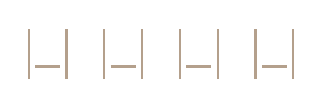
\begin{tikzpicture}[scale=0.8]
  \foreach \x in {0,1,2,3,4,5,6,7} {
    \draw[rulecolor,thick] (\x*0.6,0) -- (\x*0.6,0.8);
  }
  \foreach \x in {0,1,2,3} {
    \draw[rulecolor,thick] (\x*1.2+0.1,0.2) -- (\x*1.2+0.5,0.2);
  }
\end{tikzpicture}

\vfill
{\small\textit{Typeset from the Siku Quanshu (四庫全書) edition}}\\
{\small Bilingual edition with parallel Chinese text and English translation}

\end{titlepage}

% -------- Table of Contents --------
\tableofcontents
\newpage

% ============================================================================
\section*{Introduction / 緒言}
\addcontentsline{toc}{section}{Introduction / 緒言}
% ============================================================================

\begin{paracol}{2}

\begin{leftcolumn*}
\noindent\textbf{數學九章}為南宋秦九韶所撰，是中古數學之偉大著作。全書九章，每章一類。

本卷呈其第三、四卷：
\begin{itemize}[leftmargin=*,nosep]
  \item \textbf{卷三上：田域類} -- 方田、圓田、三角田及組合圖形之面積
  \item \textbf{卷三下：田域類續} -- 續田域問題，含籌算圖式
  \item \textbf{卷四上：測望類} -- 隔河測高遠，用勾股重差之法
  \item \textbf{卷四下：測望類續} -- 續測望問題，量不可至之遠近高下
\end{itemize}

文本依中算傳統格式：
\begin{itemize}[leftmargin=*,nosep]
  \item \textbf{問} -- 問題陳述
  \item \textbf{答} -- 答數
  \item \textbf{術} -- 演算方法
  \item \textbf{草} -- 詳細演草
\end{itemize}
\end{leftcolumn*}

\begin{rightcolumn}
The \textit{Shu Xue Jiu Zhang} (Mathematical Treatise in Nine Chapters), 
written by Qin Jiushao during the Southern Song Dynasty, 
is one of the greatest masterpieces of medieval Chinese mathematics. The work 
contains nine chapters, each devoted to a different class of problems.

This volume presents Fascicles 3 and 4 of the work, covering:
\begin{itemize}[leftmargin=*,nosep]
  \item \textbf{Juan 3 Shang -- Tian Yu (Fields, Part 1):} Problems on area measurement, 
    including squares, circles, triangles, and composite figures.
  \item \textbf{Juan 3 Xia -- Tian Yu (Fields, Part 2):} Continuation of field problems, 
    including more complex configurations with counting rod diagrams.
  \item \textbf{Juan 4 Shang -- Ce Wang (Surveying, Part 1):} Problems on remote 
    measurement and surveying, using similar triangles and the gou-gu method.
  \item \textbf{Juan 4 Xia -- Ce Wang (Surveying, Part 2):} Further surveying problems, 
    including measurement of heights, distances, and inaccessible objects.
\end{itemize}

The text follows the classical format of Chinese mathematical literature:
\begin{itemize}[leftmargin=*,nosep]
  \item \textbf{Wen (問):} The problem statement
  \item \textbf{Da Yue (答):} The answer
  \item \textbf{Shu Yue (術):} The method/algorithm
  \item \textbf{Cao Yue (草):} The working/calculation
\end{itemize}
\end{rightcolumn}

\end{paracol}

\newpage

% ============================================================================
\section{Juan 3 Shang -- Tian Yu / 卷三上田域類}
\label{sec:juan3shang}
% ============================================================================

\begin{paracol}{2}

\begin{leftcolumn*}
\noindent\textit{小序：}此卷論田域面積之術。涉方圓、斜直、面冪、體積，皆相求之。其本則出於立天元一法。
\end{leftcolumn*}

\begin{rightcolumn}
\noindent\textit{Introductory note:} This fascicle treats problems on area 
measurement (Tian Yu). The problems involve squares, circles, triangles, and 
composite figures. Qin Jiushao employs his ``method of the celestial element'' 
(Tian Yuan Shu) alongside traditional algorithmic techniques.
\end{rightcolumn}

\end{paracol}

\vspace{0.5em}

% -------- Problem 1 --------
\subsection*{Problem 1: Fang Zhong Gu Yuan / 方中古圓池}
\addcontentsline{toc}{subsection}{Problem 1: Fang Zhong Gu Yuan Chi}

\begin{paracol}{2}

\begin{leftcolumn*}
\wen / \textbf{第一問：方中古圓池}

有方中古圓池，因陂毀於一角。從外方隅斜至內圓邊七尺六寸。欲依舊修之，求圓徑、方面、方斜各幾何。
\end{leftcolumn*}

\begin{rightcolumn}
\prb\ / \textbf{Square with Inscribed Circular Pond}

There is a square field with an ancient circular pond 
inscribed within it. The northern corner has partially collapsed. From the 
corner of the outer square to the edge of the inner circle, the diagonal 
distance is 7 chi 6 cun (7.6 chi). Wishing to repair it according to 
the original design, find: the diameter of the circle, the side of the 
square, and the diagonal of the square.
\end{rightcolumn}

\switchcolumn[0]*

\begin{leftcolumn*}
\da / \textbf{答曰：}

池圓徑三丈六尺六寸，四百二十九分寸之四百一十二。

方面三丈六尺六寸，四百二十九分寸之四百一十二。

方斜五丈一尺八寸，四百二十九分寸之四百一十二。
\end{leftcolumn*}

\begin{rightcolumn}
\ans\ / \textbf{Answer:}

The pond's diameter is 36 chi 6 cun plus $\frac{412}{429}$ cun; 
the square's side is 36 chi 6 cun plus $\frac{412}{429}$ cun; the square's 
diagonal is 51 chi 8 cun plus $\frac{412}{429}$ cun.
\end{rightcolumn}

\switchcolumn[0]*

\begin{leftcolumn*}
\shu / \textbf{術曰：}

以少廣求之，太朮入之。如積斜自乘倍之為實，倍斜為一方法，一半寸為從隅。開平方得徑。
\end{leftcolumn*}

\begin{rightcolumn}
\meth\ / \textbf{Method:}

Using the ``lesser breadth'' (shao guang) method with the 
``transformation of the embryo'' (tai tai) technique. Square the diagonal 
and double it to obtain the dividend (shi). Take twice the diagonal as the 
negative coefficient of the linear term (yi fang). Take half a cun as the 
coefficient of the quadratic term (cong yu). Extract the square root to find 
the diameter.
\end{rightcolumn}

\end{paracol}

\vspace{0.5em}
\noindent\textbf{Tu (Diagram / 圖):}
\begin{center}
\begin{tikzpicture}[scale=1.0]
  \draw[thick] (0,0) rectangle (3.5,3.5);
  \draw[thick] (1.75,1.75) circle (1.3);
  \draw[thick,dashed] (0,3.5) -- (1.75,1.75);
  \fill[gray!30] (0,3.5) -- (0,2.7) -- (0.8,3.5) -- cycle;
  \node[above right,font=\small] at (0,3.5) {隅 (corner)};
  \node[font=\small] at (1.75,1.75) {圓 (circle)};
  \node[below left,font=\small] at (0.6,2.7) {斜 (diagonal)};
\end{tikzpicture}
\end{center}

\vspace{1em}

% -------- Problem 2 --------
\subsection*{Problem 2: San Xie Qiu Ji / 三斜求積}
\addcontentsline{toc}{subsection}{Problem 2: San Xie Qiu Ji}

\begin{paracol}{2}

\begin{leftcolumn*}
\wen / \textbf{第二問：三斜求積}

有三斜形田，大斜一十三里，小斜一十四里，中斜一十五里。里法三百步，欲知為田積幾何。
\end{leftcolumn*}

\begin{rightcolumn}
\prb\ / \textbf{Triangular Field Area}

There is a triangular field. The large diagonal 
(da xie) is 13 li, the small diagonal (xiao xie) is 14 li, and the middle 
diagonal (zhong xie) is 15 li. With 300 bu per li, find the area.
\end{rightcolumn}

\switchcolumn[0]*

\begin{leftcolumn*}
\da / \textbf{答曰：}

田積三百一十五頃。
\end{leftcolumn*}

\begin{rightcolumn}
\ans\ / \textbf{Answer:}

The area is 315 qing.
\end{rightcolumn}

\switchcolumn[0]*

\begin{leftcolumn*}
\shu / \textbf{術曰：}

以少廣求之。以小斜冪並大斜冪，減中斜冪，餘半之，自乘於上。以小斜冪乘大斜冪，減上，餘四約之為實。一為從隅，開平方得積。
\end{leftcolumn*}

\begin{rightcolumn}
\meth\ / \textbf{Method:}

Using the ``lesser breadth'' method. Add the squares of 
the small and large diagonals, subtract the square of the middle diagonal. 
Halve the remainder and square it (placed above). Multiply the square of 
the small diagonal by the square of the large diagonal; subtract the result 
above; divide the remainder by 4 to get the dividend. Take 1 as the 
coefficient of the quadratic term; extract the square root to find the area.

\medskip
\textit{In modern notation:} If $a=13$, $b=14$, $c=15$, then:
\[
S = \sqrt{\frac{1}{4}\left[a^2b^2 - \left(\frac{a^2+b^2-c^2}{2}\right)^2\right]}
\]
This is equivalent to \textbf{Heron's formula}:
\[
S = \sqrt{s(s-a)(s-b)(s-c)}, \quad s = \frac{a+b+c}{2}
\]
\end{rightcolumn}

\end{paracol}

\vspace{1em}

% -------- Problem 3 --------
\subsection*{Problem 3: Fang Tian Yuan Chi / 方田圓池}
\addcontentsline{toc}{subsection}{Problem 3: Fang Tian Yuan Chi}

\begin{paracol}{2}

\begin{leftcolumn*}
\wen / \textbf{第三問：方田圓池}

有方田一段，內有圓池水占之，外計地三千一百六十八步。只云從內池周至外田角斜二十一步半。內外方圆各幾何。
\end{leftcolumn*}

\begin{rightcolumn}
\prb\ / \textbf{Square Field with Central Circular Pond}

There is a square field with a circular pond inside 
it. The remaining land outside the pond amounts to 3168 bu. It is given 
that the diagonal distance from the edge of the inner pond to the corner 
of the outer square is 21.5 bu. Find the dimensions of both the inner 
circle and outer square.
\end{rightcolumn}

\switchcolumn[0]*

\begin{leftcolumn*}
\da / \textbf{答曰：}

內池周四十二步，徑一十三步半。方田面六十步。
\end{leftcolumn*}

\begin{rightcolumn}
\ans\ / \textbf{Answer:}

The inner pond's circumference is 42 bu, its diameter is 
13.5 bu; the square field's side is 60 bu.
\end{rightcolumn}

\switchcolumn[0]*

\begin{leftcolumn*}
\shu / \textbf{術曰：}

以少廣求之。置積以圓率三約之為實，倍斜為從方，斜冪為一負隅。開平方得內徑。加倍斜得方面。
\end{leftcolumn*}

\begin{rightcolumn}
\meth\ / \textbf{Method:}

Using the ``lesser breadth'' method. Place the area and 
divide by the circular rate 3 to obtain the dividend. Twice the diagonal 
gives the linear coefficient. The square of the diagonal gives the 
negative quadratic coefficient. Extract the square root to find the inner 
diameter. Add twice the diagonal to obtain the square's side.
\end{rightcolumn}

\end{paracol}

\vspace{1em}

% -------- Problem 4 --------
\subsection*{Problem 4: Piao Tian / 漂田}
\addcontentsline{toc}{subsection}{Problem 4: Piao Tian}

\begin{paracol}{2}

\begin{leftcolumn*}
\wen / \textbf{第四問：漂田}

有漂田一段，中斜一十六步，水止五步。減中斜一十六餘一十一步為元大斜。內減殘大斜二十步……
\end{leftcolumn*}

\begin{rightcolumn}
\prb\ / \textbf{The Drowned Field}

There is a ``drowned field'' (a triangular field 
partially submerged). The middle diagonal is 16 bu; the water depth is 
5 bu. Subtracting 5 from 16 gives 11 bu as the base large diagonal.
\end{rightcolumn}

\switchcolumn[0]*

\begin{leftcolumn*}
\da / \textbf{答曰：}

田積若干。
\end{leftcolumn*}

\begin{rightcolumn}
\ans\ / \textbf{Answer:}

The field area is [to be determined].
\end{rightcolumn}

\switchcolumn[0]*

\begin{leftcolumn*}
\shu / \textbf{術曰：}

草曰：以水止五減中斜一十六餘一十一步為法。以中斜一十六乘大殘二十得三百二十為大斜實。以法除之得二十九步一十一分步之一為元大斜。內減殘大斜二十步，餘九步一十一分步之一……
\end{leftcolumn*}

\begin{rightcolumn}
\meth\ / \textbf{Method:}

(Detailed calculation with specific numerical operations as recorded in the original text.)

\textit{Working:} Take the water depth 5 subtracted from the middle diagonal 16, 
remainder 11 bu as the divisor. Multiply the middle diagonal 16 by the large 
remainder 20 to get 320 as the large diagonal dividend. Divide by the divisor 
to get 29 and $\frac{1}{11}$ bu as the original large diagonal. Subtract the 
large remainder 20 bu, remainder 9 and $\frac{1}{11}$ bu...
\end{rightcolumn}

\end{paracol}

\vspace{0.5em}
\noindent\textbf{Tu (Diagram / 圖):}
\begin{center}
\begin{tikzpicture}[scale=0.8]
  \draw[thick] (0,0) -- (5.5,0) -- (1.8,3.5) -- cycle;
  \fill[blue!20] (0,0) -- (5.5,0) -- (4.2,1.3) -- (0.9,0.9) -- cycle;
  \draw[thick,dashed] (0.9,0.9) -- (4.2,1.3);
  \node[below,font=\small] at (2.75,-0.3) {水止五步};
  \node[left,font=\small] at (-0.3,1.8) {中斜};
  \node[right,font=\small] at (3.8,2.5) {大斜};
  \node[font=\small] at (2.75,0.4) {水 (water)};
\end{tikzpicture}
\end{center}

\newpage

% ============================================================================
\section{Juan 3 Xia -- Tian Yu Xu / 卷三下田域類續}
\label{sec:juan3xia}
% ============================================================================

% -------- Problem 5 --------
\subsection*{Problem 5: San Hu Fen Tian / 三戶分田}
\addcontentsline{toc}{subsection}{Problem 5: San Hu Fen Tian}

\begin{paracol}{2}

\begin{leftcolumn*}
\wen / \textbf{第五問：三戶分田}

有田一段，欲分與甲乙丙三戶。甲多一百五十步，乙多一百二十步，丙多九十步。三戶共田若干，各得幾何。
\end{leftcolumn*}

\begin{rightcolumn}
\prb\ / \textbf{Division of Land Among Three Families}

There is a field to be divided among three families 
jia, yi, and bing. Family jia receives 150 bu more than the base amount; 
family yi receives 120 bu more; family bing receives 90 bu more. If the 
total area is given, find each family's share.
\end{rightcolumn}

\switchcolumn[0]*

\begin{leftcolumn*}
\da / \textbf{答曰：}

甲田若干，乙田若干，丙田若干。
\end{leftcolumn*}

\begin{rightcolumn}
\ans\ / \textbf{Answer:}

Family jia's share [is determined]; family yi's share [is determined]; 
family bing's share [is determined].
\end{rightcolumn}

\switchcolumn[0]*

\begin{leftcolumn*}
\shu / \textbf{術曰：}

以少廣求之。併三戶多出之數以減總積，餘以三戶約之，各得本積。又各加多出之數即得各戶之田。
\end{leftcolumn*}

\begin{rightcolumn}
\meth\ / \textbf{Method:}

Using the ``lesser breadth'' method. Add the excess amounts 
from all three families and subtract from the total area. Divide the 
remainder by 3 to get the base amount for each. Add each family's excess 
to the base amount to obtain each share.
\end{rightcolumn}

\end{paracol}

\vspace{1em}

% -------- Problem 6 --------
\subsection*{Problem 6: Yuan Tian Fang Tian / 圓田方田}
\addcontentsline{toc}{subsection}{Problem 6: Yuan Tian Fang Tian}

\begin{paracol}{2}

\begin{leftcolumn*}
\wen / \textbf{第六問：圓田方田}

有方圓田各一段，共積一千二百八十步。只云方面如圓徑少四步，問方圆面徑各幾何。
\end{leftcolumn*}

\begin{rightcolumn}
\prb\ / \textbf{Circular and Square Fields}

There is a square field and a circular field. Their 
total area is 1280 bu. It is given that the square's side is 4 bu less 
than the circle's diameter. Find the side and diameter.
\end{rightcolumn}

\switchcolumn[0]*

\begin{leftcolumn*}
\da / \textbf{答曰：}

方面若干，圓徑若干。
\end{leftcolumn*}

\begin{rightcolumn}
\ans\ / \textbf{Answer:}

The square's side [and] the circle's diameter [are determined].
\end{rightcolumn}

\switchcolumn[0]*

\begin{leftcolumn*}
\shu / \textbf{術曰：}

以少廣求之。置共積以圓率三、方率四各約之為實，方面少圓徑四步為從方。開平方得圓徑。減四得方面。
\end{leftcolumn*}

\begin{rightcolumn}
\meth\ / \textbf{Method:}

Using the ``lesser breadth'' method. Place the combined 
area; divide by the circular rate 3 and square rate 4 to obtain the 
dividend. The difference of 4 bu between square side and circle diameter 
gives the linear coefficient. Extract the square root to find the diameter. 
Subtract 4 to obtain the square's side.
\end{rightcolumn}

\end{paracol}

\vspace{1em}

% -------- Problem 7 --------
\subsection*{Problem 7: Hu Tian / 弧田}
\addcontentsline{toc}{subsection}{Problem 7: Hu Tian}

\begin{paracol}{2}

\begin{leftcolumn*}
\wen / \textbf{第七問：弧田}

有弧田一段，弦五十步，矢二十五步，求積若干。
\end{leftcolumn*}

\begin{rightcolumn}
\prb\ / \textbf{Circular Segment Field}

There is a circular segment field (hu tian) with chord 
(xian) 50 bu and arrow (shi) 25 bu. Find its area.
\end{rightcolumn}

\switchcolumn[0]*

\begin{leftcolumn*}
\da / \textbf{答曰：}

田積若干。
\end{leftcolumn*}

\begin{rightcolumn}
\ans\ / \textbf{Answer:}

The field area [is determined].
\end{rightcolumn}

\switchcolumn[0]*

\begin{leftcolumn*}
\shu / \textbf{術曰：}

以弦矢求之。以弦乘矢，又以矢自乘，併之，半之為實。開平方得積。
\end{leftcolumn*}

\begin{rightcolumn}
\meth\ / \textbf{Method:}

Using the chord-arrow method. Multiply the chord by the 
arrow; add the square of the arrow; halve to obtain the dividend. Extract 
the square root to find the area.

\medskip
\textit{Note:} For a circular segment with chord $c$ and sagitta $s$, 
Qin's formula gives:
\[
A = \frac{cs + s^2}{2}
\]
This is an approximation to the true area of a circular segment.
\end{rightcolumn}

\end{paracol}

\vspace{0.5em}
\noindent\textbf{Counting Rod Diagram / 籌算圖式:}
\begin{center}
\begin{tabular}{|c|c|c|c|}
\hline
\textbf{弦} & \textbf{矢} & \textbf{弦乘矢} & \textbf{矢冪} \\
\hline
50 & 25 & 1250 & 625 \\
\hline
\multicolumn{2}{|c|}{\textbf{併}} & \textbf{半之} & \textbf{積} \\
\hline
\multicolumn{2}{|c|}{1875} & 937.5 & $\approx$ 30.6 \\
\hline
\end{tabular}
\end{center}

\newpage

% ============================================================================
\section{Juan 4 Shang -- Ce Wang / 卷四上測望類}
\label{sec:juan4shang}
% ============================================================================

\begin{paracol}{2}

\begin{leftcolumn*}
\noindent\textit{小序：}此卷論測望之術，量不可至之高遠。用勾股、重差之法，為中國古代測量學之基礎。
\end{leftcolumn*}

\begin{rightcolumn}
\noindent\textit{Introductory note:} This fascicle treats problems on 
surveying and remote measurement (Ce Wang). These problems involve measuring 
inaccessible distances and heights using the ``hook-and-gourd'' (gou gu) 
method and similar triangles.
\end{rightcolumn}

\end{paracol}

\vspace{0.5em}

% -------- Problem 1 --------
\subsection*{Problem 1: Yuan Cheng / 圓城}
\addcontentsline{toc}{subsection}{Problem 1: Yuan Cheng}

\begin{paracol}{2}

\begin{leftcolumn*}
\wen / \textbf{第一問：圓城}

有圓城不知周徑，四門中開。北外三里有喬木，出南門折而東行九里乃見木。欲知城周徑各幾何。
\end{leftcolumn*}

\begin{rightcolumn}
\prb\ / \textbf{The Round City}

There is a circular city of unknown circumference 
and diameter. It has four gates at the cardinal points. Three li north 
of the north gate stands a tall tree. Going out the south gate and then 
turning east for 9 li, the tree becomes visible. Find the circumference 
and diameter of the city.
\end{rightcolumn}

\switchcolumn[0]*

\begin{leftcolumn*}
\da / \textbf{答曰：}

徑九里，周二十七里。
\end{leftcolumn*}

\begin{rightcolumn}
\ans\ / \textbf{Answer:}

The diameter is 9 li, the circumference is 27 li.
\end{rightcolumn}

\switchcolumn[0]*

\begin{leftcolumn*}
\shu / \textbf{術曰：}

以勾股夕桀求之。一為從隅，五因北里為從七廉，置北里冪八因為從五廉，以北里乘上廉為一從，三連負隅乘五廉為一上廉，以北里乘上廉為實。開玲瓏九乘方得數，自乘為徑。以三因徑得周。
\end{leftcolumn*}

\begin{rightcolumn}
\meth\ / \textbf{Method:}

Using the ``hook-and-gourd evening-peak'' method. Take 1 
as the leading coefficient. Multiply the north distance by 5 for the 
seventh-degree coefficient. Place the square of the north distance, 
multiply by 8 for the fifth-degree coefficient. Multiply the north 
distance by the upper coefficient for the negative linear coefficient. 
Double the negative rate to form the fifth-degree coefficient as the 
negative upper coefficient. Multiply the north distance by the upper 
coefficient for the dividend. Extract the ninth-degree root (ling long kai fang) 
to obtain the number; square it for the diameter. Multiply the diameter 
by 3 for the circumference.
\end{rightcolumn}

\end{paracol}

\vspace{1em}

% -------- Problem 2 --------
\subsection*{Problem 2: Ce Ta / 測塔}
\addcontentsline{toc}{subsection}{Problem 2: Ce Ta}

\begin{paracol}{2}

\begin{leftcolumn*}
\wen / \textbf{第二問：測塔}

有塔高未知其數，去塔若干步立一表，人目上望見塔尖，退行若干步又立一表，人目上望仍見塔尖。求塔高及去塔遠近。
\end{leftcolumn*}

\begin{rightcolumn}
\prb\ / \textbf{Measuring a Tower}

A tower of unknown height stands at an unknown 
distance. At a certain distance from the tower, a pole is erected; 
looking upward from eye level, the tower's peak is visible. Retreating 
a certain distance and erecting another pole, the peak is again visible 
from eye level. Find the tower's height and distance.
\end{rightcolumn}

\switchcolumn[0]*

\begin{leftcolumn*}
\da / \textbf{答曰：}

塔高若干，去塔遠若干。
\end{leftcolumn*}

\begin{rightcolumn}
\ans\ / \textbf{Answer:}

The tower height [and] distance to the tower [are determined].
\end{rightcolumn}

\switchcolumn[0]*

\begin{leftcolumn*}
\shu / \textbf{術曰：}

以勾股求之。兩表退行之差為法，前表去塔遠乘表高，後表去塔遠乘表高，相減為實。實如法而一得塔高。又以法除前表去塔遠乘兩表高差加表高得塔高。
\end{leftcolumn*}

\begin{rightcolumn}
\meth\ / \textbf{Method:}

Using the hook-and-gourd method. The difference between 
the retreat distances of the two poles is the divisor. Multiply the 
front pole's distance to the tower by the pole height; multiply the rear 
pole's distance by the pole height; subtract to obtain the dividend. 
Divide to get the tower height. Alternatively, multiply the front distance 
by the difference of pole heights, divide by the divisor, and add the 
pole height.

\medskip
\textit{In modern notation:} Let $d_1$ = front distance, $d_2$ = rear 
distance, $h$ = pole height. Then:
\[
\text{Tower height} = \frac{d_2 \cdot h - d_1 \cdot h}{d_2 - d_1} = h
\]
This uses the principle of similar triangles, where the ratio of heights 
equals the ratio of distances.
\end{rightcolumn}

\end{paracol}

\vspace{1em}

% -------- Problem 3 --------
\subsection*{Problem 3: Fang Cheng / 方城}
\addcontentsline{toc}{subsection}{Problem 3: Fang Cheng}

\begin{paracol}{2}

\begin{leftcolumn*}
\wen / \textbf{第三問：方城}

有方城一座，不知大小。北門外有樹，出南門直行若干步折而西行若干步見樹。求城方面。
\end{leftcolumn*}

\begin{rightcolumn}
\prb\ / \textbf{The Square City}

There is a square city of unknown size. Outside the 
north gate stands a tree. Going out the south gate and walking straight 
a certain number of steps, then turning west and walking a certain 
number of steps, the tree becomes visible. Find the side of the square 
city.
\end{rightcolumn}

\switchcolumn[0]*

\begin{leftcolumn*}
\da / \textbf{答曰：}

城方面若干步。
\end{leftcolumn*}

\begin{rightcolumn}
\ans\ / \textbf{Answer:}

The city's side is [determined] in bu.
\end{rightcolumn}

\switchcolumn[0]*

\begin{leftcolumn*}
\shu / \textbf{術曰：}

以勾股求之。兩行步相乘為實，併兩行步為從方。開平方得城方面。
\end{leftcolumn*}

\begin{rightcolumn}
\meth\ / \textbf{Method:}

Using the hook-and-gourd method. Multiply the two walk 
distances for the dividend. Add the two walk distances for the linear 
coefficient. Extract the square root to obtain the city's side.

\medskip
If $a$ = southward steps and $b$ = westward steps:
\[
x^2 + (a+b)x = ab \quad\Rightarrow\quad x = \frac{-(a+b) + \sqrt{(a+b)^2 + 4ab}}{2}
\]
\end{rightcolumn}

\end{paracol}

\vspace(1em)

% -------- Problem 4 --------
\subsection*{Problem 4: Chou Suan Kai Fang / 籌算開方}
\addcontentsline{toc}{subsection}{Problem 4: Chou Suan Kai Fang}

\begin{paracol}{2}

\begin{leftcolumn*}
\wen / \textbf{第四問：籌算開方}

問以開方術解高次方程，其籌佈列之法若何。
\end{leftcolumn*}

\begin{rightcolumn}
\prb\ / \textbf{Counting Rod Root Extraction}

On the method of extracting roots to solve higher-degree 
equations, how are the counting rods arranged?
\end{rightcolumn}

\switchcolumn[0]*

\begin{leftcolumn*}
\shu / \textbf{術曰：}

開方之法，先列實於中，次列隅於下，次列方於上。商除之，以上乘隅生廉，以上乘廉生方，以上乘方除實。實盡則止，不盡則倍方，三廉為方法，續商除之。
\end{leftcolumn*}

\begin{rightcolumn}
\meth\ / \textbf{Method:}

In the method of root extraction, first place the dividend 
(shi) in the middle, then place the unit coefficient (yu) below, and the 
linear coefficient (fang) above. Divide by estimation; multiply the estimate 
by the unit coefficient to generate the linear coefficient; multiply the 
estimate by the linear coefficient and subtract from the dividend. When 
the dividend is exhausted, stop. If not exhausted, double the linear 
coefficient and proceed to the next digit.
\end{rightcolumn}

\end{paracol}

\vspace{0.5em}
\noindent\textbf{Counting Rod Layout / 籌式:}
\begin{center}
\begin{tabular}{|c|c|c|c|c|}
\hline
\textbf{商} & \textbf{實} & \textbf{方} & \textbf{廉} & \textbf{隅} \\
\hline
7 & 360 & 130 & ... & 1 \\
\hline
\multicolumn{5}{|c|}{\textit{Iterative extraction / 逐次開方}} \\
\hline
\end{tabular}
\end{center}

\textit{Note:} In the counting rod system, vertical strokes represent units 
($1,2,3,4$) and horizontal strokes represent fives. The symbol T 
represents 6 (5+1). The diagram shows the iterative process of root extraction.

\newpage

% ============================================================================
\section{Juan 4 Xia -- Ce Wang Xu / 卷四下測望類續}
\label{sec:juan4xia}
% ============================================================================

% -------- Problem 5 --------
\subsection*{Problem 5: Ce Shui Shen / 測水深}
\addcontentsline{toc}{subsection}{Problem 5: Ce Shui Shen}

\begin{paracol}{2}

\begin{leftcolumn*}
\wen / \textbf{第五問：測水深}

有井不知其深，以繩測之，繩長倍於井深餘三尺；三摺而測之適足。求井深及繩長。
\end{leftcolumn*}

\begin{rightcolumn}
\prb\ / \textbf{Measuring Depth of Water}

There is a well of unknown depth. Measuring with a 
rope, the rope's length is twice the well's depth with 3 chi to spare. 
Folding the rope in three and measuring, it fits exactly. Find the depth 
of the well and the length of the rope.
\end{rightcolumn}

\switchcolumn[0]*

\begin{leftcolumn*}
\da / \textbf{答曰：}

井深三尺，繩長九尺。
\end{leftcolumn*}

\begin{rightcolumn}
\ans\ / \textbf{Answer:}

The well is 3 chi deep; the rope is 9 chi long.
\end{rightcolumn}

\switchcolumn[0]*

\begin{leftcolumn*}
\shu / \textbf{術曰：}

以盈不足求之。倍繩餘三尺為盈，三摺適足為適足。以盈乘適足為實，併盈適足為法，除之得井深。倍之加盈得繩長。
\end{leftcolumn*}

\begin{rightcolumn}
\meth\ / \textbf{Method:}

Using the ``surplus and deficit'' (ying bu zu) method. The 
3 chi excess when doubled is the surplus; the exact fit when tripled is 
the exact amount. Multiply the surplus by the exact amount for the 
dividend; add surplus and exact amount for the divisor; divide to obtain 
the well depth. Double and add the excess for the rope length.

\medskip
\textit{In modern notation:} Let $d$ = well depth, $L$ = rope length.
\[
L = 2d + 3, \qquad \frac{L}{3} = d
\]
Substituting: $2d + 3 = 3d \Rightarrow d = 3$, $L = 9$.
\end{rightcolumn}

\end{paracol}

\vspace{1em}

% -------- Problem 6 --------
\subsection*{Problem 6: Ce Ta Gao / 測塔高}
\addcontentsline{toc}{subsection}{Problem 6: Ce Ta Gao}

\begin{paracol}{2}

\begin{leftcolumn*}
\wen / \textbf{第六問：測塔高}

有塔高未知，去塔百步立一表高五尺，人目去表一尺八寸，上望塔尖與表端參合。退行六十步，人目去表端仍參合塔尖。求塔高及塔心去表遠近。
\end{leftcolumn*}

\begin{rightcolumn}
\prb\ / \textbf{Measuring the Height of a Pagoda}

A pagoda of unknown height stands at an unknown 
distance. 100 bu from the pagoda, a 5-chi pole is erected. The observer's 
eye is 1.8 chi from the ground; looking up, the pagoda's peak aligns 
with the pole's tip. Retreating 60 bu, the observer's eye again aligns 
with both the pole's tip and the pagoda's peak. Find the pagoda's height 
and its distance from the pole.
\end{rightcolumn}

\switchcolumn[0]*

\begin{leftcolumn*}
\da / \textbf{答曰：}

塔身高三丈，塔高一十一丈七尺，與八丈七尺為塔心目長。
\end{leftcolumn*}

\begin{rightcolumn}
\ans\ / \textbf{Answer:}

The pagoda's body is 3 zhang high; the total height 
(from ground to peak) is 11 zhang 7 chi; the distance from the pagoda's 
center to the measuring point is 8 zhang 7 chi.
\end{rightcolumn}

\switchcolumn[0]*

\begin{leftcolumn*}
\shu / \textbf{術曰：}

此皆大小形同勢相求法也。人目去塔為總股，人目去杆為分小股，人目上塔尖高塔身節為總股高。相論高為分大勾，數一杆去塔分大勾於小角杆去塔為分大勾。
\end{leftcolumn*}

\begin{rightcolumn}
\meth\ / \textbf{Method:}

These are all applications of similar triangles (da xiao xing tong shi). 
The distance from eye to pagoda is the total height line; the distance 
from eye to pole is the small height line. The height from eye level to 
pagoda peak is the total height; the height from eye level to pole top 
is the small height. The method uses proportional relationships between 
these quantities.

\medskip
\textit{This problem uses the principle of similar triangles:}
\[
\frac{\text{Pagoda height} - \text{eye height}}{\text{Distance to pagoda}} = 
\frac{\text{Pole height} - \text{eye height}}{\text{Distance to pole}}
\]
\end{rightcolumn}

\end{paracol}

\vspace(1em)

% -------- Problem 7 --------
\subsection*{Problem 7: Ge He Ce Yuan / 隔河測遠}
\addcontentsline{toc}{subsection}{Problem 7: Ge He Ce Yuan}

\begin{paracol}{2}

\begin{leftcolumn*}
\wen / \textbf{第七問：隔河測遠}

問隔河望一高岸，不知其遠。平地立一表，人目上望見岸頂，又退立一表望之仍見岸頂。求河闊及岸高。
\end{leftcolumn*}

\begin{rightcolumn}
\prb\ / \textbf{Measuring Distance Across a River}

Across a river, a high bank is visible at an unknown 
distance. A pole is erected on level ground; looking up from eye level, 
the bank's top is visible. Retreating and erecting another pole, the 
bank's top is again visible. Find the width of the river and the height 
of the bank.
\end{rightcolumn}

\switchcolumn[0]*

\begin{leftcolumn*}
\da / \textbf{答曰：}

河闊若干步，岸高若干尺。
\end{leftcolumn*}

\begin{rightcolumn}
\ans\ / \textbf{Answer:}

The river width [and] the bank height [are determined].
\end{rightcolumn}

\switchcolumn[0]*

\begin{leftcolumn*}
\shu / \textbf{術曰：}

以重差求之。兩表退行步數之差為法，前表去岸遠乘表高為實，實如法而一得岸高。又以法除後表去岸遠乘表高亦得岸高，兩者相驗。
\end{leftcolumn*}

\begin{rightcolumn}
\meth\ / \textbf{Method:}

Using the ``double difference'' (chong cha) method. The 
difference between the two retreat distances is the divisor. Multiply 
the front pole's distance to the bank by the pole height for the dividend; 
divide to obtain the bank height. Similarly for the rear pole; the two 
results should agree (providing verification).
\end{rightcolumn}

\end{paracol}

\vspace(1em)

% -------- Problem 8 --------
\subsection*{Problem 8: Jiu Cheng Fang / 九乘方}
\addcontentsline{toc}{subsection}{Problem 8: Jiu Cheng Fang}

\begin{paracol}{2}

\begin{leftcolumn*}
\wen / \textbf{第八問：九乘方}

問以開九乘方術解方程，其立法之原若何。
\end{leftcolumn*}

\begin{rightcolumn}
\prb\ / \textbf{The Nine-Degree Root Method}

On the method of extracting ninth-degree roots to 
solve equations --- what is the fundamental principle of this method?
\end{rightcolumn}

\switchcolumn[0]*

\begin{leftcolumn*}
\shu / \textbf{術曰：}

開方之術，至於九乘方，其理一也。先列實於中，次定隅位，次立方廉法。商除之際，以上乘隅生廉，以上乘廉生方，以上乘方除實。每進一位，則方退一，廉退二，隅退三。如是疊進，直至實盡為止。
\end{leftcolumn*}

\begin{rightcolumn}
\meth\ / \textbf{Method:}

The method of root extraction, up to the ninth degree, 
follows the same principle. First place the dividend in the middle; 
then determine the unit position; then establish the linear and 
intermediate coefficients. During division-by-estimation: multiply the 
estimate by the unit coefficient to generate the intermediate 
coefficients; multiply the estimate by the intermediate coefficients to 
generate the linear coefficient; multiply the estimate by the linear 
coefficient and subtract from the dividend. At each decimal shift, the 
linear coefficient descends one place, the intermediate descend two 
places, and the unit descends three. Continue iteratively until the 
dividend is exhausted.

\medskip
\textit{Note:} This describes \textbf{Horner's method} for solving polynomial 
equations, which Qin Jiushao developed independently centuries before 
Horner. For a polynomial:
\[
a_n x^n + a_{n-1} x^{n-1} + \cdots + a_1 x + a_0 = 0
\]
The method systematically reduces the polynomial by factoring out 
$(x - r)$ where $r$ is the estimated root at each step.
\end{rightcolumn}

\end{paracol}

\vspace{0.5em}
\noindent\textbf{Layout for Ninth-Degree Root Extraction / 九乘方籌式:}
\begin{center}
\begin{tabular}{|c|c|c|c|c|c|c|c|c|c|}
\hline
商 & 實 & 方 & 一廉 & 二廉 & 三廉 & 四廉 & 五廉 & 六廉 & 隅 \\
\hline
7 & -- & 153 & ... & ... & ... & ... & ... & ... & 1 \\
\hline
\multicolumn{10}{|c|}{\textit{Iterative computation with place-value shifts / 逐位遞推}} \\
\hline
\end{tabular}
\end{center}

\newpage

% ============================================================================
\section*{Appendix / 附錄: Mathematical Notes}
\addcontentsline{toc}{section}{Appendix / 附錄: Mathematical Notes}
% ============================================================================

\begin{paracol}{2}

\begin{leftcolumn*}
\subsection*{A.1 籌算 / The Counting Rod System}

籌算為中國古代主要計算工具。以竹籌佈列十進位制：
\begin{itemize}[leftmargin=*,nosep]
  \item \textbf{一至四：} 縱式 $|$, $||$, $|||$, $||||$
  \item \textbf{五：} 橫式 $\equiv$
  \item \textbf{六至九：} 組合，如 T（五加一）
  \item \textbf{零：} 以空位或圓 $\bigcirc$ 表之
\end{itemize}

籌列於算板，每列一位。此位值制助成高深代數運算，如開方、解方程。
\end{leftcolumn*}

\begin{rightcolumn}
\subsection*{A.1 The Counting Rod System (Chou Suan)}

The counting rod system (Chou Suan) was the primary computational tool in 
ancient Chinese mathematics. Numbers were represented by bamboo sticks 
arranged in a decimal place-value system:
\begin{itemize}[leftmargin=*,nosep]
  \item \textbf{Units ($1$--$4$):} Vertical strokes $|$, $||$, 
    $|||$, $||||$
  \item \textbf{Fives:} A horizontal stroke $=$ placed over the units
  \item \textbf{6--9:} Combinations, e.g., T (5+1), 
    $\equiv$ (3 horizontal over vertical)
  \item \textbf{Zero:} Represented by a blank space or circle $\bigcirc$
\end{itemize}

The rods were arranged on a counting board in columns, with each column 
representing a decimal place. This positional system enabled sophisticated 
algebraic computations including root extraction and solution of polynomial 
equations.
\end{rightcolumn}

\switchcolumn[0]*

\begin{leftcolumn*}
\subsection*{A.2 天元術 / The Celestial Element Method}

秦九韶精於天元術，為早期代數符號。未知數謂之「天元」，方程以籌式佈列。此法可解十次方程，早霍納五百餘年。
\end{leftcolumn*}

\begin{rightcolumn}
\subsection*{A.2 The ``Celestial Element'' Method (Tian Yuan Shu)}

Qin Jiushao was a master of the ``celestial element'' method, an early form 
of algebraic symbolism. The unknown quantity was called ``celestial element'' 
(Tian Yuan, tian yuan), and equations were set up using counting rod arrangements. 
This method could solve polynomial equations of degree up to 10, anticipating 
Horner's method by over 500 years.
\end{rightcolumn}

\switchcolumn[0]*

\begin{leftcolumn*}
\subsection*{A.3 三斜求積公式 / Qin's Formula for Triangular Area}

三角形三邊 $a$, $b$, $c$，秦九韶公式：
\[
S = \sqrt{\frac{1}{4}\left[c^2a^2 - \left(\frac{c^2+a^2-b^2}{2}\right)^2\right]}
\]
此與海龍公式等價，顯十三世紀非凡代數造詣。
\end{leftcolumn*}

\begin{rightcolumn}
\subsection*{A.3 Qin Jiushao's Formula for Triangular Area}

For a triangle with sides $a$, $b$, $c$, Qin gave the formula:
\[
S = \sqrt{\frac{1}{4}\left[c^2a^2 - \left(\frac{c^2+a^2-b^2}{2}\right)^2\right]}
\]
This is equivalent to Heron's formula and demonstrates remarkable algebraic 
insight for the 13th century.
\end{rightcolumn}

\switchcolumn[0]*

\begin{leftcolumn*}
\subsection*{A.4 盈不足術 / The Surplus and Deficit Method}

盈不足術為通用線性問題解法。設兩試值得盈、不足，則真值：
\[
x = \frac{a_2b_1 + a_1b_2}{a_1 + a_2}
\]
其中 $a_1$, $a_2$ 為試入之數，$b_1$, $b_2$ 為對應盈不足之數。
\end{leftcolumn*}

\begin{rightcolumn}
\subsection*{A.4 The ``Surplus and Deficit'' Method (Ying Bu Zu)}

The method of surplus and deficit (Ying Bu Zu Shu) is a general technique for 
solving linear problems. Given two trial values yielding surplus and deficit 
results, the true value is found by:
\[
x = \frac{a_2b_1 + a_1b_2}{a_1 + a_2}
\]
where $a_1$, $a_2$ are the trial inputs and $b_1$, $b_2$ are the 
corresponding surplus/deficit amounts. This method can be applied to 
a wide variety of practical problems.
\end{rightcolumn}

\end{paracol}

\vspace{1cm}

\begin{center}
{\color{rulecolor}\rule{10cm}{0.4pt}}\\[0.5cm]
{\small\textit{End of Fascicles 3--4 / 卷三至四終}}\\[0.3cm]
{\small Shu Xue Jiu Zhang -- Juan 3 Shang, Juan 3 Xia, Juan 4 Shang, Juan 4 Xia / 數學九章}
\end{center}

\end{document}



% ============================================================
% Source: translations/en/chinese/qin-jiushao-shuxue-jiuzhang-fascicles5-6_bilingual.tex
% ============================================================

%% =============================================================================
%% 數學九章 (Shuxue Jiuzhang) — Fascicles 5-6: Bilingual Edition
%% LEFT: Original Chinese  |  RIGHT: English Translation
%% Author: Qin Jiushao (秦九韶), Song Dynasty
%% Source: Siku Quanshu (四庫全書) Edition
%% =============================================================================
\documentclass[10pt,a4paper]{article}

%% -------- Core Packages --------
\usepackage{fontspec}
\usepackage{polyglossia}
\usepackage{amsmath,amssymb}
\usepackage{geometry}
\usepackage{graphicx}
\usepackage{xcolor}
\usepackage{titlesec}
\usepackage{fancyhdr}
\usepackage{enumitem}
\usepackage{array,booktabs,longtable,multirow}
\usepackage{hyperref}
\usepackage{tocloft}
\usepackage{indentfirst}
\usepackage{xeCJK}
\usepackage{paracol}
\usepackage{tikz}
\usepackage{microtype}

%% -------- Page Geometry (wider for two-column bilingual) --------
\geometry{
  paperwidth=297mm,paperheight=210mm,  % Landscape A4
  left=18mm,right=18mm,top=20mm,bottom=20mm,
  headheight=14pt,footskip=20pt
}

%% -------- Column separator --------
\setlength{\columnsep}{4mm}

%% -------- Language Setup --------
\setmainlanguage{english}
\setotherlanguage{chinese}

%% -------- Font Configuration --------
\setmainfont{LinLibertine_R.otf}[
  BoldFont=LinLibertine_RB.otf,
  ItalicFont=LinLibertine_RI.otf,
  BoldItalicFont=LinLibertine_RBI.otf,
  Renderer=Harfbuzz
]
\setsansfont{LinBiolinum_R.otf}[
  BoldFont=LinBiolinum_RB.otf,
  ItalicFont=LinBiolinum_RI.otf,
  Renderer=Harfbuzz
]

%% Chinese Fonts (using specified CJK font)
\setCJKmainfont[Path=/mnt/agents/fonts/noto-sc-extracted/]{NotoSansCJKsc-Regular.otf}
\setCJKsansfont[Path=/mnt/agents/fonts/noto-sc-extracted/]{NotoSansCJKsc-Regular.otf}
\setCJKmonofont[Path=/mnt/agents/fonts/noto-sc-extracted/]{NotoSansCJKsc-Regular.otf}

%% -------- Colors --------
\definecolor{titlecolor}{RGB}{45,55,72}
\definecolor{sectioncolor}{RGB}{55,65,81}
\definecolor{notecolor}{RGB}{120,53,15}
\definecolor{rulecolor}{RGB}{180,160,140}
\definecolor{problemcolor}{RGB}{80,40,20}
\definecolor{answercolor}{RGB}{20,80,40}
\definecolor{methodcolor}{RGB}{20,40,80}
\definecolor{editorcolor}{RGB}{100,60,40}
\definecolor{workingcolor}{RGB}{60,60,60}

%% -------- Section Formatting --------
\titleformat{\section}
  {\normalfont\Large\bfseries\color{sectioncolor}}
  {\thesection}{1em}{}
\titleformat{\subsection}
  {\normalfont\large\bfseries\color{sectioncolor}}
  {\thesubsection}{1em}{}
\titleformat{\subsubsection}
  {\normalfont\normalsize\bfseries\color{problemcolor}}
  {\thesubsubsection}{1em}{}

%% -------- Header/Footer --------
\pagestyle{fancy}
\fancyhf{}
\fancyhead[L]{\small\textsc{Shuxue Jiuzhang 數學九章 --- Fascicles 5--6 (Bilingual Edition)}}
\fancyhead[R]{\small\thepage}
\renewcommand{\headrulewidth}{0.4pt}
\renewcommand{\footrulewidth}{0pt}

%% -------- Custom Commands --------
\newcommand{\longline}{\noindent\rule{\textwidth}{0.4pt}}
\newcommand{\shortline}{\noindent\rule{0.5\textwidth}{0.4pt}\par}
\newcommand{\cnote}[1]{\textcolor{notecolor}{\textit{#1}}}

%% Bilingual section header
\newcommand{\BilingualHeader}[2]{%
  \vspace{1em}%
  \noindent\begin{center}%
  \begin{minipage}[t]{0.45\textwidth}\centering\textbf{\color{sectioncolor}#1}\end{minipage}%
  \hfill%
  \begin{minipage}[t]{0.45\textwidth}\centering\textbf{\color{sectioncolor}#2}\end{minipage}%
  \end{center}%
  \vspace{0.5em}%
}

%% Small bilingual header for subsections
\newcommand{\BilingualSubheader}[2]{%
  \vspace{0.8em}%
  \noindent\begin{center}%
  \begin{minipage}[t]{0.45\textwidth}\centering\large\bfseries\color{sectioncolor}#1\end{minipage}%
  \hfill%
  \begin{minipage}[t]{0.45\textwidth}\centering\large\bfseries\color{sectioncolor}#2\end{minipage}%
  \end{center}%
  \vspace{0.3em}%
}

%% -------- Problem structure commands (Chinese - LEFT) --------
\newcommand{\QuestionCn}[1]{\par\noindent\textbf{\color{problemcolor}問：}#1\par}
\newcommand{\AnswerCn}[1]{\par\noindent\textbf{\color{answercolor}答曰：}#1\par}
\newcommand{\MethodCn}[1]{\par\noindent\textbf{\color{methodcolor}術曰：}#1\par}
\newcommand{\WorkingCn}[1]{\par\noindent\textbf{\color{workingcolor}草曰：}#1\par}
\newcommand{\EditorialCn}[1]{\par\noindent\textit{\color{editorcolor}［按］#1}\par}

%% -------- Problem structure commands (English - RIGHT) --------
\newcommand{\QuestionEn}[1]{\par\noindent\textbf{\color{problemcolor}Problem: }#1\par}
\newcommand{\AnswerEn}[1]{\par\noindent\textbf{\color{answercolor}Answer: }#1\par}
\newcommand{\MethodEn}[1]{\par\noindent\textbf{\color{methodcolor}Method: }#1\par}
\newcommand{\WorkingEn}[1]{\par\noindent\textbf{\color{workingcolor}Working: }#1\par}
\newcommand{\EditorialEn}[1]{\par\noindent\textit{\color{editorcolor}[Ed.\ Note] #1}\par}

%% -------- Bilingual environment --------
\newenvironment{Bilingual}{%
  \par\vspace{0.5em}%
  \noindent%
  \begin{minipage}[t]{0.47\textwidth}%
}{%
  \end{minipage}%
  \hfill%
  \begin{minipage}[t]{0.47\textwidth}%
}{%
  \end{minipage}%
  \par\vspace{0.5em}%
}

\newcommand{\ChineseCol}[1]{%
  \begin{minipage}[t]{0.47\textwidth}#1\end{minipage}%
}
\newcommand{\EnglishCol}[1]{%
  \begin{minipage}[t]{0.47\textwidth}#1\end{minipage}%
}

%% -------- Vertical divider --------
\newcommand{\vdivider}{%
  \tikz[remember picture,overlay]\draw[rulecolor,line width=0.4pt] (current page header area.south -| 0.5\paperwidth,0) -- (current page footer area.north -| 0.5\paperwidth,0);%
}

%% -------- Hyperref Setup --------
\hypersetup{
  colorlinks=true,
  linkcolor=sectioncolor,
  citecolor=sectioncolor,
  urlcolor=sectioncolor,
  pdfencoding=auto,
  pdftitle={Shuxue Jiuzhang --- Fascicles 5-6 (Bilingual Edition)},
  pdfauthor={Qin Jiushao (秦九韶)},
  pdfsubject={Chinese Mathematics}
}

%% -------- TOC Depth --------
\setcounter{tocdepth}{2}
\setcounter{secnumdepth}{2}

%% Reduce paragraph spacing for dense text
\setlength{\parskip}{0.4ex plus 0.2ex minus 0.1ex}
\setlength{\parindent}{1.5em}

%% =============================================================================
\begin{document}

%% -------- Title Page --------
\begin{titlepage}
\centering
\vspace*{2cm}

{\fontsize{28}{34}\selectfont\color{titlecolor}\textbf{數學九章}}

\vspace{0.8cm}

{\fontsize{14}{18}\selectfont\color{sectioncolor} Mathematical Treatise in Nine Sections}

\vspace{1.5cm}

{\Large\color{sectioncolor}
\textbf{Bilingual Edition} / 雙語版}

\vspace{1.5cm}

{\large\color{sectioncolor}
卷五：\textbf{賦役} (Fascicle 5: Taxation and Corv\'{e}e)\quad|\quad
卷六：\textbf{錢穀} (Fascicle 6: Money and Grain)
}

\vspace{2cm}

{\large 宋\quad 秦九韶\quad 撰}

\vspace{0.3cm}

{\normalsize\textit{Qin Jiushao (c.\ 1202--1261)}}

\vspace{0.3cm}

{\small\color{sectioncolor} Translated and Annotated}

\vspace{2cm}

{\color{rulecolor}\rule{0.5\textwidth}{0.4pt}}

\vspace{1cm}

{\small\color{sectioncolor}
\textit{Siku Quanshu} (四庫全書) Edition\\[0.5em]
Digital Scholarly Edition\quad|\quad Bilingual Layout: Chinese (Left) $\|$ English (Right)
}

\vspace{2cm}

{\small\color{notecolor}
\textit{This document preserves the traditional Chinese mathematical\\
text structure of 問 (Problem), 答 (Answer), 術 (Method), and 草 (Working).}
}

\vfill
{\small\color{sectioncolor} Typeset in XeLaTeX with Noto Sans CJK SC \& Libertine}
\end{titlepage}

%% -------- Table of Contents --------
\tableofcontents
\newpage

%% =============================================================================
%% BILINGUAL MACRO SETUP
%% =============================================================================
%% We use a two-column layout: LEFT = Chinese, RIGHT = English
%% Each "BilingualSection" takes {ChineseContent}{EnglishContent}
\newcommand{\BilingualSection}[4]{%
  \newpage
  \subsection*{#1 \hfill #2}
  \addcontentsline{toc}{subsection}{#3}
  \vspace{0.5em}
  \longline
  \vspace{0.5em}
}

\newcommand{\BilingualBlock}[2]{%
  \noindent\begin{minipage}[t]{0.47\textwidth}#1\end{minipage}%
  \hfill\vrule width 0.4pt\hfill%
  \noindent\begin{minipage}[t]{0.47\textwidth}#2\end{minipage}%
  \par\vspace{0.8em}%
}

\newcommand{\ProblemBlock}[2]{%
  \noindent\begin{minipage}[t]{0.47\textwidth}#1\end{minipage}%
  \hfill\hfill%
  \noindent\begin{minipage}[t]{0.47\textwidth}#2\end{minipage}%
  \par\vspace{0.5em}%
}

%% =============================================================================
%% EDITORIAL PREFACE
%% =============================================================================
\section*{Editorial Preface / 編輯前言}
\addcontentsline{toc}{section}{Editorial Preface / 編輯前言}

\ProblemBlock{%
\textbf{\color{sectioncolor}卷五上：賦役}\quad 賦役一章，即古九章中差分粟米諸法。但從來算書設題之數未有如此卷之多者。如首題答數至一百七十五條，毎條歩算之數至十餘位，而得數皆無不合，亦可謂能廣其用矣。且諸問皆足以明貴賤廩税及交質變易之同異，使公私各得其平，誠治民之要務也。

\vspace{0.5em}
\textbf{\color{sectioncolor}卷五下：賦役}\quad 題語多晦，術草中間有與所問不相應者，亦於各條下指出，俾觀者無惑焉。

\vspace{0.5em}
\textbf{\color{sectioncolor}卷六上：錢穀}\quad 差人五路和糴，課貴賤，折輕齎，皆國家理財之要道。

\vspace{0.5em}
\textbf{\color{sectioncolor}卷六下：錢穀}\quad 推求本息，易牒知原，粟米交易，計米易麴，囘運費，三色均價。凡此皆市易之術，亦古粟米章之遺意也。%
}{%
\textbf{\color{sectioncolor}Fascicle 5 (Upper): Fuyi (Tax and Corv\'{e}e)}\\
The chapter on Tax and Corv\'{e}e Labor draws upon the classical Nine Chapters' methods of \textit{proportional distribution} (差分, \textit{chaifen}) and \textit{millet and rice} (粟米, \textit{sumi}). Never before has a mathematical treatise presented problems of such complexity---the first problem alone yields 175 separate numerical results, each calculated to more than ten digits, all mutually consistent. These problems illuminate the principles of fair taxation, grain assessment, and commercial exchange, ensuring equity between public and private interests---truly essential matters of governance.

\vspace{0.5em}
\textbf{\color{sectioncolor}Fascicle 5 (Lower): Fuyi}\\
The problem statements are often obscure, and occasionally the methods and workings do not fully correspond to the questions asked. These discrepancies are noted in the editorial annotations below.

\vspace{0.5em}
\textbf{\color{sectioncolor}Fascicle 6 (Upper): Qiangu (Money and Grain)}\\
Government grain procurement across five circuits, price comparison, and currency conversion---all essential methods of state financial management.

\vspace{0.5em}
\textbf{\color{sectioncolor}Fascicle 6 (Lower): Qiangu}\\
Calculating principal and interest, chain-exchange problems, grain transactions, rice-for-yeast calculations, return shipping costs, and averaging gold of three purity grades---these are all commercial methods, inheriting the spirit of the classical Millet and Rice chapter.%
}

\newpage
%% =============================================================================
%% FASCICLE 5 — 賦役 (TAXATION AND CORVÉE LABOR)
%% =============================================================================
\section*{\color{titlecolor}卷五\quad 賦役類 / Fascicle 5: Taxation and Corv\'{e}e Labor}
\addcontentsline{toc}{section}{卷五\quad 賦役類 / Fascicle 5: Taxation and Corv\'{e}e Labor}

\noindent\rule{\textwidth}{1pt}
\vspace{0.3em}

%% ---------------------------------------------------------------------------
%% PROBLEM 1: 復邑修賦
%% ---------------------------------------------------------------------------
\subsection*{\color{sectioncolor}復邑修賦 / Restoring a District and Calculating Tax Obligations}
\addcontentsline{toc}{subsection}{復邑修賦 / Restoring a District}

\ProblemBlock{%
\QuestionCn{%
有海坍縣地，今有復漲，歳乆鄉井再成，申諸剏邑。稱土排到六鄉，以附郭為甲，最逺為已，各有田九等，開具下項：

\vspace{0.3em}
甲鄉共計田十四萬一百九十三畝三角一十二步。上等：上田五千六百七十八畝一角四十八歩；中田四千八百九十二畝三十歩；下田六千六百二十一畝五十四歩。中等：上田八千二百二十五畝二十四歩；中田一萬三十五畝六歩；下田一萬六千五百三十畝。下等：上田二萬一千九十畝二十四歩；中田三萬二千六十畝三歩；下田三萬五千六十一畝三角三歩。

乙鄉田共計八萬四千一十畝二角二歩。丙鄉田共計一十二萬九百三十五畝五十八歩五分。丁鄉田共計八萬九千六十六畝二歩三分。戊鄉田共計二十萬四千四百七十四畝一角二十四歩四分。已鄉田共計一十五萬八千四百六十畝三角一十八歩二分。

照得昨來本縣原科苗米一十萬三千五百六十七石八斗四升四合三勺，和買一萬三千四百九十八匹一丈七尺三寸七分六釐，夏税九千八百七十六匹三丈二尺六寸五分八釐。其六鄉田係三色，甲為上，乙丙為次，丁戊己又為次。先令官物為三差，使上比中、中比下皆十分外差一，次令各鄉九等皆於十分内差一，抛科用合租額。其乙鄉田最肥，次丁，次甲，次丙，次己，次戊。欲知三色九等毎畝等則及共科數各鄉幾何？
}
}{%
\QuestionEn{%
A coastal county's land had eroded into the sea; now new land has re-emerged from the tides. After many years, villages and settlements have re-formed, and a petition has been submitted to establish a new county. The land survey has classified six villages (xiang), with village Jia (甲) nearest the city walls and village Ji (己) furthest away. Each village has land of nine grades. The details are as follows:

\vspace{0.3em}
\textbf{Village Jia:} Total land 140,193 mu 3 jiao 12 bu. Upper grade: upper fields 5,678 mu 1 jiao 48 bu; middle fields 4,892 mu 30 bu; lower fields 6,621 mu 54 bu. Middle grade: upper fields 8,225 mu 24 bu; middle fields 10,035 mu 6 bu; lower fields 16,530 mu. Lower grade: upper fields 21,090 mu 24 bu; middle fields 32,060 mu 3 bu; lower fields 35,061 mu 3 jiao 3 bu.

\textbf{Villages Yi, Bing, Ding, Wu, Ji:} [similar detailed land classifications follow, with Yi totaling 84,010 mu 2 jiao 2 bu; Bing 120,935 mu 58\nicefrac{5}{10} bu; Ding 89,066 mu 2\nicefrac{3}{10} bu; Wu 204,474 mu 1 jiao 24\nicefrac{4}{10} bu; Ji 158,460 mu 3 jiao 18\nicefrac{2}{10} bu.]

The county's original tax quotas were: seedling rice (苗米) 103,567 shi 8 dou 4 sheng 4 ge 3 shao; harmonized purchase (和買) 13,498 pi 1 zhang 7 chi 3 cun 7 fen 6 li; summer tax (夏税) 9,876 pi 3 zhang 2 chi 6 cun 5 fen 8 li. The six villages are grouped into three tiers: Jia is upper tier; Yi and Bing are middle tier; Ding, Wu, and Ji are lower tier. First, the official goods are divided into three graduated differentials (san chai), with upper to middle and middle to lower each differing by one part in ten. Then each village's nine grades differ by one part in ten. The land quality ranks: Yi has the most fertile land, followed by Ding, Jia, Bing, Ji, and Wu. Find: the tax rate per mu for each of the three tiers and nine grades, and the total tax collected from each village.
}
}

\ProblemBlock{%
\EditorialCn{%
題内言田有三色，甲為上云云，又言乙鄉田最肥云云，語若相左。葢前言三色者六鄉共科之等，後言田肥者每畝所出之異也。若易田係三色為科有三差，則語意明矣。%
}
}{%
\EditorialEn{%
The problem states that the fields are of three colors (tiers), with Jia as the upper tier, but also states that Yi village has the most fertile land---these two statements appear contradictory. The former refers to the collective tax tier of the six villages; the latter refers to the per-mu yield of each village's land. Replacing ``fields are of three colors'' with ``taxation has three graduated differentials'' would clarify the meaning.%
}
}

\ProblemBlock{%
\AnswerCn{%
甲鄉：上等上田苗三斗二升三合二勺，和一尺六寸九分，税一尺二寸三分；中田苗二斗九升九勺，和一尺五寸二分，税一尺一寸一分；下田苗二斗五升八合六勺，和一尺三寸五分，税九寸九分。

中等上田苗二斗二升六合二勺，和一尺一寸八分，税八寸六分；中田苗一斗九升三合九勺，和一尺一分，税七寸四分；下田苗一斗六升一合六勺，和八寸四分，税六寸二分。

下等上田苗一斗二升九合三勺，和六寸七分，税四寸九分；中田苗九升六合九勺，和五寸一分，税三寸七分；下田苗六升四合六勺，和三寸四分，税二寸五分。

\textit{[Similar detailed results follow for villages Yi, Bing, Ding, Wu, and Ji, each with rates for all nine grades of land.]}

各鄉共科數：甲鄉苗米一萬九千五百五十石二斗四升八合三勺；和買一萬一百九十二丈二尺六寸五分六釐；夏税七千四百五十七丈六尺八寸九分八釐。

乙、丙、丁、戊、己各鄉共科數依上法求之。
}
}{%
\AnswerEn{%
\textbf{Village Jia:} Upper-grade upper fields: rice 3 dou 2 sheng 3 ge 2 shao; silk 1 chi 6 cun 9 fen; tax silk 1 chi 2 cun 3 fen. Upper-grade middle fields: rice 2 dou 9 sheng 0 ge 9 shao; silk 1 chi 5 cun 2 fen; tax silk 1 chi 1 cun 1 fen. Upper-grade lower fields: rice 2 dou 5 sheng 8 ge 6 shao; silk 1 chi 3 cun 5 fen; tax silk 9 cun 9 fen.

Middle-grade upper fields: rice 2 dou 2 sheng 6 ge 2 shao; silk 1 chi 1 cun 8 fen; tax silk 8 cun 6 fen. Middle-grade middle fields: rice 1 dou 9 sheng 3 ge 9 shao; silk 1 chi 1 cun 0 fen; tax silk 7 cun 4 fen. Middle-grade lower fields: rice 1 dou 6 sheng 1 ge 6 shao; silk 8 cun 4 fen; tax silk 6 cun 2 fen.

Lower-grade upper fields: rice 1 dou 2 sheng 9 ge 3 shao; silk 6 cun 7 fen; tax silk 4 cun 9 fen. Lower-grade middle fields: rice 9 sheng 6 ge 9 shao; silk 5 cun 1 fen; tax silk 3 cun 7 fen. Lower-grade lower fields: rice 6 sheng 4 ge 6 shao; silk 3 cun 4 fen; tax silk 2 cun 5 fen.

\textit{[Similar results for villages Yi, Bing, Ding, Wu, and Ji follow.]}

\textbf{Village Jia totals:} Seedling rice 19,550 shi 2 dou 4 sheng 8 ge 3 shao; Harmonized purchase 10,192 zhang 2 chi 6 cun 5 fen 6 li; Summer tax 7,457 zhang 6 chi 8 cun 9 fen 8 li.

The totals for villages Yi, Bing, Ding, Wu, and Ji are found by the same method.
}
}

\ProblemBlock{%
\MethodCn{%
以衰分求之。先列本縣色位，自下錐行列之，又以鄉數對列而乗之，副併為法，以除官物數，得一分之率。以率數乗未併者，各得諸鄉之數。次列各鄉等位，自上等置十分，每以内分錐行九折之，至九等止，又各以畝歩乗之，副併為鄉法，以除諸各鄉所得官物數，所得為一分之率，以乗未併者，各得毎畝税色。%
}
}{%
\MethodEn{%
Use the method of proportional distribution (衰分, \textit{chuifen}). First arrange the county's tier positions in a descending cone array; multiply by the corresponding village counts. Sum these to form the divisor; divide the official goods by this divisor to obtain the rate for one part. Multiply the rate by the un-summed terms to obtain each village's quota. Next, arrange each village's nine grades, starting from the upper grade at 10 parts, successively reducing by one-tenth for each grade down to the ninth grade. Multiply each by the field area in mu and bu. Sum these as the village divisor; divide each village's goods by this divisor to obtain the rate per grade. Multiply by the un-summed terms to obtain the tax per mu for each grade.%
}
}

\ProblemBlock{%
\WorkingCn{%
列本縣色位三，自下色例十分中十一分，上比中身外加一，上得一百二十一，中得一百一十，下得一百，為上中下三率，列之右行。乃列甲一對上率，乙丙共二對中率，丁戊己共三對下率，列左行。乃以左行列數各相對乗右行率數，其上得一百二十一，其十得二百二十，其下得三百，乃副置而併之，得六百四十一為法。

置元科苗米一十萬三千五百六十七石八斗四升四合三勺為寔，以法除之，得一百六十一石五斗七升二合三勺為一分之率。以未併下率一百乗率，得一萬六千一百五十七石二斗三升為丁戊己三鄉各科數。於身下加一，得一萬七千七百七十二石九斗五升三合為乙丙二鄉各科數。又於身下加一，得一萬九千五百五十石二斗四升八合三勺為甲合科數。

求和買亦用六百四十一為法，置元科和買一萬三千四百九十八匹，以匹法四丈通之，得五萬三千九百九十二丈，内零一丈七尺三寸七分六釐，得五萬三千九百九十三丈七尺三寸七分六釐為寔，以法除之，得八十四丈二尺三寸三分六釐為一分之率。亦以未併下率一百乗之，得八千四百二十三丈三尺六寸為丁戊己三鄉各科數。次於身下加一，得九千二百六十五丈六尺九寸六分為乙丙二鄉各科數。又於身下加一，得一萬一百九十二丈二尺六寸五分六釐為甲鄉合科數。

求夏税亦置六百四十一為法，置元科九千八百七十六匹，以匹法四丈通之，得三萬九千五百四丈，内零三丈二尺六寸五分八釐，得三萬九千五百七丈二尺六寸五分八釐為寔，以法除之，得六十一丈六尺三寸三分八釐為一分率。亦以未併下率一百乗之，得六千一百六十三丈三尺八寸為丁戊己三鄉各科數。次於身下加一，得六千七百七十九丈七尺一寸八分为乙丙二鄉各科數。又於身下加一，得七千四百五十七丈六尺八寸九分八釐為甲鄉數。%
}
}{%
\WorkingEn{%
Arrange the three county tiers in a descending cone array, with the lower tier as 100, middle as 110 (adding one-tenth), and upper as 121 (adding another one-tenth), yielding the three rates for upper, middle, and lower tiers in the right column. In the left column, pair Jia (1) with the upper rate, Yi and Bing (2) with the middle rate, and Ding, Wu, and Ji (3) with the lower rate. Cross-multiply: upper yields 121, middle yields 220, lower yields 300. Sum these to obtain 641 as the divisor.

Take the original seedling rice quota 103,567 shi 8 dou 4 sheng 4 ge 3 shao as the dividend; divide by 641 to obtain 161 shi 5 dou 7 sheng 2 ge 3 shao as the rate for one part. Multiply the unsummed lower rate of 100: 16,157 shi 2 dou 3 sheng for Ding, Wu, and Ji villages. Add one-tenth: 17,772 shi 9 dou 5 sheng 3 ge for Yi and Bing. Add another one-tenth: 19,550 shi 2 dou 4 sheng 8 ge 3 shao for Jia.

For the harmonized purchase: again use 641 as divisor. Convert the original 13,498 pi to zhang (at 4 zhang per pi): 53,992 zhang, plus the remainder 1 zhang 7 chi 3 cun 7 fen 6 li = 53,993 zhang 7 chi 3 cun 7 fen 6 li. Divide by 641: 84 zhang 2 chi 3 cun 3 fen 6 li as the unit rate. Multiply by lower rate 100: 8,423 zhang 3 chi 6 cun for Ding, Wu, Ji. Add one-tenth: 9,265 zhang 6 chi 9 cun 6 fen for Yi, Bing. Add one-tenth: 10,192 zhang 2 chi 6 cun 5 fen 6 li for Jia.

For summer tax: use 641 as divisor. Convert 9,876 pi to zhang: 39,504 zhang, plus remainder 3 zhang 2 chi 6 cun 5 fen 8 li = 39,507 zhang 2 chi 6 cun 5 fen 8 li. Divide by 641: 61 zhang 6 chi 3 cun 3 fen 8 li as the rate. Multiply by lower rate 100: 6,163 zhang 3 chi 8 cun for Ding, Wu, Ji. Add one-tenth: 6,779 zhang 7 chi 1 cun 8 fen for Yi, Bing. Add one-tenth: 7,457 zhang 6 chi 8 cun 9 fen 8 li for Jia.%
}
}

\newpage
%% ---------------------------------------------------------------------------
%% PROBLEM 2: 圍田租畝
%% ---------------------------------------------------------------------------
\subsection*{\color{sectioncolor}圍田租畝 / Rental Calculations for Enclosed Fields}
\addcontentsline{toc}{subsection}{圍田租畝 / Rental Calculations for Enclosed Fields}

\ProblemBlock{%
\QuestionCn{%
有興復圍田已成，共計三千二十一頃五十一畝一十五歩，分三等。其上等毎畆起租六斗，中等四斗五升，下等四斗。中田多上田弱半，不及下田太半。欲知三色田畝及各租幾何？%
}
}{%
\QuestionEn{%
A newly reclaimed enclosed polder field has been completed, totaling 3,021 qing 51 mu 15 bu, divided into three grades. The upper grade pays rent of 6 dou per mu; the middle grade 4 dou 5 sheng; the lower grade 4 dou. The middle-grade fields exceed the upper-grade fields by one weak half (weak half = one-third); the middle-grade fields fall short of the lower-grade fields by one great half (great half = two-thirds). Find: the area of each grade of field and the rental grain for each.%
}
}

\ProblemBlock{%
\EditorialCn{%
題言中田多上田弱半，不及下田太半。蓋以弱半為三分之一，太半為三分之二也。多上田弱半者，即比上田多三分之一也。不及下田太半者，即比下田少三分之二也。是上田加三分之一為中田，即下田三分之一也。轉言之，則中田為下田三分之一，上田為中田四分之三也。%
}
}{%
\EditorialEn{%
The problem states that middle-grade fields exceed upper-grade fields by one ``weak half,'' and fall short of lower-grade fields by one ``great half.'' Here ``weak half'' means one-third, and ``great half'' means two-thirds. Exceeding the upper fields by one weak half means exceeding by one-third; falling short of the lower fields by one great half means falling short by two-thirds. Thus: upper fields plus one-third equals middle fields, which equals one-third of the lower fields. Equivalently: middle fields are one-third of lower fields, and upper fields are three-quarters of middle fields.%
}
}

\ProblemBlock{%
\AnswerCn{%
上田四百七十七頃八畝一十五歩，米二萬八千六百二十四石八斗三升七合五勺；
中田六百三十六頃一十畝三角，米二萬八千六百二十四石八斗三升七合五勺；
下田一千九百八頃三十二畝一角，米七萬六千三百三十二石九斗。%
}
}{%
\AnswerEn{%
Upper fields: 477 qing 8 mu 15 bu, grain 28,624 shi 8 dou 3 sheng 7 ge 5 shao;
Middle fields: 636 qing 10 mu 3 jiao, grain 28,624 shi 8 dou 3 sheng 7 ge 5 shao;
Lower fields: 1,908 qing 32 mu 1 jiao, grain 76,332 shi 9 dou.\par
\textit{Note: Upper and middle fields happen to yield equal total rents because the area difference compensates for the rate difference.}%
}
}

\ProblemBlock{%
\MethodCn{%
以衰分求之。列母子求田率，副併為法，以共田為寔，寔如法而一，得一分之率。以徧乗未併者，得三等田。各以起租乗之，各得米。%
}
}{%
\MethodEn{%
Use proportional distribution (衰分, \textit{chuifen}). Arrange the numerators and denominators to find the field ratios. Sum these as the divisor; take the total fields as the dividend. Divide to obtain the rate for one part. Multiply the un-summed terms by this rate to obtain the three grades of fields. Multiply each by its rental rate to obtain the grain for each grade.%
}
}

\ProblemBlock{%
\WorkingCn{%
置弱半母四為中率，子三為上率。以太半子二减母三，餘一，以乗中率四，只得四為中泛。又以餘一乗上率三，只得三為上泛。次以太半母三乗中泛四，得一十二為下泛。副併三泛，得一十九為法。置田三千二十一頃五十一畆，以畝法二百四十通之，得七千二百五十一萬六千二百四十歩，内子一十五歩，得七千二百五十一萬六千二百五十五歩為寔。以法一十九除之，得三百八十一萬六千六百四十五歩為一分之數。以上泛三因之，得一千一百四十四萬九千九百三十五歩為上積。又以中泛四因之一分數，得一千五百二十六萬六千五百八十歩為中積。又以下泛一十二乗一分數，得四千五百七十九萬九千七百四十歩為下積。其三積各以畝法二百四十約之為畆。其上田得四百七十七頃八畝一十五歩，其中田得六百三十六頃一十畝三角，其下積得一千九百八頃三十二畝一角。各以起租，三積為三寔。其上積一千一百四十四萬九千九百三十五歩乗上積六斗，得六百八十六萬九千九百六十一石為寔，以畝法二百四十除之，得二萬八千六百二十四石八斗三升七合五勺為上田租。其中積一千五百二十六萬六千五百八十歩乗中田租四斗五升，得六百八十六萬九千九百六十一石為寔，以畝法二百四十除之，得二萬八千六百二十四石八斗三升七合五勺。其下積四千五百七十九萬九千七百四十歩乗下租四斗，得一千八百三十一萬九千八百九十六石為寔，以畝法二百四十除之，得七萬六千三百三十二石九斗為下田米。%
}
}{%
\WorkingEn{%
Take the ``weak half'' denominator 4 as the middle rate, numerator 3 as the upper rate. From the ``great half'' subtract numerator 2 from denominator 3, remainder 1; multiply by middle rate 4 to obtain 4 as the middle ``pan.'' Multiply remainder 1 by upper rate 3 to obtain 3 as the upper ``pan.'' Then multiply the ``great half'' denominator 3 by middle pan 4 to obtain 12 as the lower pan. Sum the three pans: 19 as the divisor.

Take the fields 3,021 qing 51 mu; convert to bu at 240 bu per mu: 72,516,240 bu, plus 15 bu = 72,516,255 bu as the dividend. Divide by 19: 3,816,645 bu as the unit rate. Multiply by upper pan 3: 11,449,935 bu as the upper product. Multiply by middle pan 4: 15,266,580 bu as the middle product. Multiply by lower pan 12: 45,799,740 bu as the lower product. Convert back to mu at 240 bu/mu: upper fields = 477 qing 8 mu 15 bu; middle = 636 qing 10 mu 3 jiao; lower = 1,908 qing 32 mu 1 jiao.

For rents: Upper product 11,449,935 bu $\times$ 6 dou = 68,699,610 shi (as dividend), divided by 240 = 28,624 shi 8 dou 3 sheng 7 ge 5 shao. Middle product $\times$ 4 dou 5 sheng gives same total by coincidence. Lower product 45,799,740 bu $\times$ 4 dou = 1,831,989,600 shi, divided by 240 = 76,332 shi 9 dou.%
}
}

\ProblemBlock{%
\EditorialCn{%
草内求各衰數，意謂以三分為上田衰數，加弱半三分之一得四分為中田衰數，三因中田衰數得一十二分為下田衰數，併之得一十九分為總衰數。其法本属顯明，但語中參入母子副泛等名目，其意反晦矣。%
}
}{%
\EditorialEn{%
The working's method of finding the distribution ratios means: taking 3 parts as the upper field ratio, adding one-third (weak half) to obtain 4 parts as the middle field ratio, tripling the middle ratio to obtain 12 parts as the lower field ratio, summing to 19 parts as the total ratio. The method is essentially clear, but the introduction of ``numerator/denominator,'' ``auxiliary,'' and ``pan'' terminology obscures the underlying simplicity.%
}
}

\newpage
%% ---------------------------------------------------------------------------
%% PROBLEM 3: 戶稅移割
%% ---------------------------------------------------------------------------
\subsection*{\color{sectioncolor}戶稅移割 / Transferring Household Tax Obligations}
\addcontentsline{toc}{subsection}{戶稅移割 / Transferring Household Tax Obligations}

\ProblemBlock{%
\QuestionCn{%
某縣據甲稱：本户田地原納苗三十五石七斗，和買本色一十一匹二丈二尺九寸四分八釐七毫五絲，折帛二十七匹二寸一分三釐七毫五絲，紬絹折帛八匹三丈九寸七寸三分九釐，紬絹本色二十匹二丈八尺九寸三分九釐。已将田四百七畆出與乙，五百十六畆出與丙。訖乞移割本户所出田上税賦，歸併乙丙兩户送納。㑹到乙原有田三百七十五畆，丙原有田四百六十三畆，並係本鄉本等。毎畆苗三升五合，税一尺一寸五分，物力一貫二百；本等田紬一尺三寸四分，物力九百；物力及三十二貫數和買一匹，内三分本色七分折帛；夏税七分本色三分折帛；紬五分本色五分折帛，併絹紬。欲知甲田地及甲乙丙分割合納苗米、和買、夏税、折帛、本色、畸零各幾何？%
}
}{%
\QuestionEn{%
In a certain county, household Jia reports: originally the household paid seedling rice 35 shi 7 dou on fields; harmonized purchase in kind 11 pi 2 zhang 2 chi 9 cun 4 fen 8 li 7 hao 5 si of silk, converted silk 27 pi 2 cun 1 fen 3 li 7 hao 5 si; pongee silk (in kind and converted) [further details]. Jia has already sold 407 mu to household Yi and 516 mu to household Bing. He petitions to transfer the tax obligations on the sold land so that Yi and Bing assume the tax payments.

Investigation reveals: Yi originally had 375 mu; Bing originally had 463 mu. All fields are of the same local grade. Per mu: seedling rice 3 sheng 5 ge; tax silk 1 chi 1 cun 5 fen; property value 1 guan 200 wen; grade-appropriate pongee silk 1 chi 3 cun 4 fen; property value 900 wen. For every 32 guan of property value: 1 pi of harmonized purchase, 3 parts in kind and 7 parts converted. Summer tax: 7 parts in kind, 3 parts converted. Pongee silk: 5 parts in kind, 5 parts converted, combined with plain silk. Find: Jia's remaining fields, and the divided tax obligations (seedling rice, harmonized purchase, summer tax, converted silk, in-kind silk, and remainders) for all three households.%
}
}

\ProblemBlock{%
\EditorialCn{%
此題科税分田地二項。田有科米、税絹、物力三色，地只有税紬、物力二色，絹與紬折色不同，物力和買合田地總計之。又甲户有田者有地，乙丙二户有田無地。此等皆不可不明言者，題中殊未分晰。%
}
}{%
\EditorialEn{%
This problem's tax assessment has two categories: fields (田) and land (地). Fields are assessed for rice, tax silk, and property value (three items); land is assessed only for pongee silk tax and property value (two items). Plain silk and pongee silk have different conversion rates. Property value for harmonized purchase combines both fields and land. Furthermore, household Jia possesses both fields and land, while households Yi and Bing possess only fields with no land. These distinctions should have been stated explicitly but were not.%
}
}

\ProblemBlock{%
\AnswerCn{%
甲原有田一千二十畆，地一十一畆二角四十八步。

甲今有田九十七畆，苗米三石三斗九升五合，夏税折帛三丈三尺四寸六分五釐，本色一匹畸零三丈八尺八分五釐，物力一百一十六貫四百文。地一十一畆二角四十八步，税紬折帛七尺八寸三分九釐，税紬畸零七尺八寸三分九釐，物力一十貫五百三十文，田地共物力一百二十六貫九百三十文。和買折帛二匹三丈一尺六分三釐七毫五絲，本色一疋畸零七尺五寸九分八釐七毫五絲。

乙今有田七百八十二畆，苗米二十七石三斗七升，夏税折帛六匹二丈九尺七寸九分，本色一十五匹畸零二丈九尺五寸一分，物力九百三十八貫四百文，和買折帛二十匹二丈一尺一寸，本色八匹畸零三丈一尺九寸。

丙今有田九百七十九畆，苗米三十四石二斗六升五合，夏税折帛八匹一丈七尺七寸五分五釐，本色一十九匹畸零二丈八尺九分五釐，物力一千一百七十四貫八百文，和買折帛二十五匹二丈七尺九寸五分，本色一十一匹畸零五寸五分。%
}
}{%
\AnswerEn{%
\textbf{Jia originally:} Fields 1,020 mu, land 11 mu 2 jiao 48 bu.

\textbf{Jia now:} Fields 97 mu; seedling rice 3 shi 3 dou 9 sheng 5 ge; summer tax converted silk 3 zhang 3 chi 4 cun 6 fen 5 li; in-kind silk 1 pi remainder 3 zhang 8 chi 8 cun 5 fen; property value 116 guan 400 wen. Land 11 mu 2 jiao 48 bu; pongee converted silk 7 chi 8 cun 3 fen 9 li; pongee remainder 7 chi 8 cun 3 fen 9 li; land property value 10 guan 530 wen. Combined property value 126 guan 930 wen. Harmonized purchase: converted silk 2 pi 3 zhang 1 chi 6 cun 3 fen 7 hao 5 si; in-kind 1 pi remainder 7 chi 5 cun 9 fen 8 li 7 hao 5 si.

\textbf{Yi now:} Fields 782 mu; seedling rice 27 shi 3 dou 7 sheng; summer tax converted silk 6 pi 2 zhang 9 chi 7 cun 9 fen; in-kind silk 15 pi remainder 2 zhang 9 chi 5 cun 1 fen; property value 938 guan 400 wen; harmonized purchase converted silk 20 pi 2 zhang 1 chi 1 cun; in-kind 8 pi remainder 3 zhang 1 chi 9 cun.

\textbf{Bing now:} Fields 979 mu; seedling rice 34 shi 2 dou 6 sheng 5 ge; summer tax converted silk 8 pi 1 zhang 7 chi 7 cun 5 fen 5 li; in-kind silk 19 pi remainder 2 zhang 8 chi 9 cun 5 fen; property value 1,174 guan 800 wen; harmonized purchase converted silk 25 pi 2 zhang 7 chi 9 cun 5 fen; in-kind 11 pi remainder 5 cun 5 fen.%
}
}

\ProblemBlock{%
\MethodCn{%
以粟米及衰分求之。置甲原納米為實，以毎畆苗為法除之，得甲原有田。以乗毎畆税，得田絹。次以甲紬絹本色折帛併之，内減田絹，餘為地紬。以毎紬約之，得甲原有地。次以甲出田併乙丙原有田，各得三户今有田地。各以等則乗之，各得物力苗税。次以毎畆物力率約各户共物力，得和買。副之，三分因之退位為和本，七分因之退位為和折；夏税反其分而因之退之；紬以半之，併入税，各得。%
}
}{%
\MethodEn{%
Use the methods of Millet and Rice (粟米, \textit{sumi}) and proportional distribution (衰分, \textit{chuifen}). Take Jia's original rice payment as dividend; divide by the per-mu seedling rate to obtain Jia's original fields. Multiply by per-mu tax silk to obtain the field silk. Combine Jia's pongee and plain silk (in-kind and converted), subtract the field silk; the remainder is land pongee. Divide by per-unit pongee to obtain Jia's original land. Add Jia's sold fields to Yi and Bing's original fields to obtain each household's current holdings. Multiply by the grade rates to obtain property values and taxes. Use the per-mu property value rate to find each household's total property value, thence the harmonized purchase. Split this: 3 parts in-kind, 7 parts converted; summer tax reverses these proportions (7 in-kind, 3 converted); pongee silk is halved (5 in-kind, 5 converted), combined with plain silk tax. These yield the final results.%
}
}

\newpage
%% ---------------------------------------------------------------------------
%% PROBLEM 4: 均科綿税
%% ---------------------------------------------------------------------------
\subsection*{\color{sectioncolor}均科綿税 / Equalizing Cotton Tax Assessment}
\addcontentsline{toc}{subsection}{均科綿税 / Equalizing Cotton Tax Assessment}

\ProblemBlock{%
\QuestionCn{%
縣科綿有五等户，共一萬一千三十三户，共科綿八萬八千三百三十七兩六錢。上等一十二户，副等八十七户，中等四百六十四户，次等二千三十五户，下等八千四百三十五户。欲令上三等折半差，下二等比中等六四折差。科率求之，問各户納及各等幾何？%
}
}{%
\QuestionEn{%
A county levies cotton floss (綿) tax on five grades of households, totaling 11,033 households, with a total assessment of 88,337 liang 6 qian. The household counts are: upper grade 12 households; sub-upper grade 87 households; middle grade 464 households; sub-middle grade 2,035 households; lower grade 8,435 households. It is desired that the upper three grades differ by successive halving (折半差), while the lower two grades are set at four-sixths (六四折) of the middle grade. Using these rates, find: the amount paid by each household grade and the total for each grade.%
}
}

\ProblemBlock{%
\EditorialCn{%
題言下二等比中等六四折差，是次等為中等六分之四，下等又為次等六分之四也。乃術草中皆以十分之四收之，是四分折差而非四六折差矣。集中題與術不相應者多類此，豈成書之後未能重加校正歟？%
}
}{%
\EditorialEn{%
The problem states that the lower two grades are at four-sixths (\nicefrac{4}{6}) of the middle grade, meaning the sub-middle grade is \nicefrac{4}{6} of the middle grade, and the lower grade is \nicefrac{4}{6} of the sub-middle grade. However, in the method and working, both are reduced by four-tenths (\nicefrac{4}{10}), which is a four-tenths reduction rather than a four-sixths reduction. Many problems in this collection have such discrepancies between the stated problem and the computational method---perhaps the author was unable to perform a thorough revision after completion.%
}
}

\ProblemBlock{%
\AnswerCn{%
上等一户一百二十四兩，一十二户計一千四百八十八兩；
副等一户六十二兩，八十七户計五千三百九十四兩；
中等一户三十一兩，四百六十四户計一萬四千三百八十四兩；
次等一户一十二兩四錢，二千三十五户計二萬五千二百三十四兩；
下等一户四兩九錢六分，八千四百三十五户計四萬一千八百三十七兩六錢。%
}
}{%
\AnswerEn{%
Upper grade: 124 liang per household, 12 households totaling 1,488 liang;
Sub-upper grade: 62 liang per household, 87 households totaling 5,394 liang;
Middle grade: 31 liang per household, 464 households totaling 14,384 liang;
Sub-middle grade: 12 liang 4 qian per household, 2,035 households totaling 25,234 liang;
Lower grade: 4 liang 9 qian 6 fen per household, 8,435 households totaling 41,837 liang 6 qian.%
}
}

\ProblemBlock{%
\MethodCn{%
列五等户數，先以四折下等數，加次等户，又以四折之，加中等户數，却以半折之，加二等户，又以半折之，加上等户數，不折便為法。除科綿，得上等一户之綿。復半之為副等，又半之為中等，又四折之為次等，又四折之為下等。各一户綿，却各以户數乗之，各得五等共出綿。%
}
}{%
\MethodEn{%
Arrange the five household grades. First reduce the lower grade by four-tenths, add to the sub-middle grade, reduce again by four-tenths, add to the middle grade. Then halve, add to the sub-upper grade; halve again, add to the upper grade. The undiscounted sum is the divisor. Divide the total cotton by this to obtain the upper-grade household's assessment. Halve for sub-upper; halve again for middle; reduce by four-tenths for sub-middle; reduce by four-tenths again for lower. Multiply each per-household amount by the respective household count to obtain each grade's total contribution.%
}
}

\ProblemBlock{%
\WorkingCn{%
先置下等户八千四百三十五，以四折之，得三千三百七十四。乃以得數折入次户二千三十五内，得五千四百九户訖。又以四折次數五千四百九户，得二千一百六十三户六分。乃以得次數併入中户四百六十四内，共得二千六百二十七户六分。次以五分折中數二千六百二十七户六分，得數。次以得數一千三百一十三户八分併副户八十七，得一千四百户八分。又以五折副數一千四百户八分，得七百户四分，既得數。乃以副數七百户四分併上户一十二户，得七百一十二户四分，不折便為法。

累折至等，共得七百一十二户四分以為總法。乃置科綿八萬八千三百三十七兩六錢為實，法七百一十二户四分而一，得一百二十四兩為上等一户所出綿。以五折之，得六十二兩為副等一户所出綿。又五折之，得三十一兩為中等一户所出綿。乃以四折之，得一十二兩四錢為次等一户所出綿。又以四折之，得四兩九錢六分為下等一户所出綿。乃以各等户數各乗一户所出，即各得每等共數之綿。%
}
}{%
\WorkingEn{%
Take lower-grade households 8,435; reduce by four-tenths: 3,374. Add to sub-middle households 2,035: 5,409. Reduce by four-tenths: 2,163.6. Add to middle households 464: 2,627.6. Halve: 1,313.8. Add to sub-upper households 87: 1,400.8. Halve: 700.4. Add to upper households 12: 712.4; this is the divisor.

The cumulative reduction yields 712.4 as the total divisor. Take the cotton assessment 88,337 liang 6 qian as dividend; divide by 712.4: 124 liang as the upper-grade per-household assessment. Halve: 62 liang (sub-upper). Halve: 31 liang (middle). Reduce by four-tenths: 12 liang 4 qian (sub-middle). Reduce by four-tenths: 4 liang 9 qian 6 fen (lower). Multiply each by the respective household count to obtain each grade's total contribution.%
}
}

\newpage
%% ---------------------------------------------------------------------------
%% PROBLEM 5: 均定勸分
%% ---------------------------------------------------------------------------
\subsection*{\color{sectioncolor}均定勸分 / Equalizing Charitable Contribution Quotas}
\addcontentsline{toc}{subsection}{均定勸分 / Equalizing Charitable Contribution Quotas}

\ProblemBlock{%
\QuestionCn{%
欲勸糶賑濟，據甲民户物力畆步排定，共計一百六十二户，作九等：上等三户，第二等五户，第三等七户，第四等八户，第五等十三户，第六等二十一户，第七等二十六户，第八等三十四户，第九等四十五户。今先觀諭，第一等上户願糶五千石，第九等户願糶二百石。欲知各等抛差石數併數認米數各幾何？%
}
}{%
\QuestionEn{%
It is desired to encourage households to sell grain for famine relief. Household Jia's property values and land have been surveyed, totaling 162 households divided into nine grades: upper grade 3 households; 2nd grade 5 households; 3rd grade 7 households; 4th grade 8 households; 5th grade 13 households; 6th grade 21 households; 7th grade 26 households; 8th grade 34 households; 9th grade 45 households. The uppermost household voluntarily offers 5,000 shi; the 9th-grade household offers 200 shi. Find: the graduated difference in grain quotas between grades, and the total recognized grain contribution for each grade.%
}
}

\ProblemBlock{%
\AnswerCn{%
認該米二十三萬七千六百石。

上等一户米五千石，三户計一萬五千石；
二等一户米四千四百石，五户計二萬二千石；
三等一户米三千八百石，七户計二萬六千六百石；
四等一户米三千二百石，八户計二萬五千六百石；
五等一户米二千六百石，一十三户計三萬三千八百石；
六等一户米二千石，二十一户計四萬二千石；
七等一户米一千四百石，二十六户計三萬六千四百石；
八等一户米八百石，三十四户計二萬七千二百石；
九等一户米二百石，四十五户計九千石。%
}
}{%
\AnswerEn{%
Total recognized grain: 237,600 shi.

Upper grade: 5,000 shi per household, 3 households totaling 15,000 shi;
2nd grade: 4,400 shi per household, 5 households totaling 22,000 shi;
3rd grade: 3,800 shi per household, 7 households totaling 26,600 shi;
4th grade: 3,200 shi per household, 8 households totaling 25,600 shi;
5th grade: 2,600 shi per household, 13 households totaling 33,800 shi;
6th grade: 2,000 shi per household, 21 households totaling 42,000 shi;
7th grade: 1,400 shi per household, 26 households totaling 36,400 shi;
8th grade: 800 shi per household, 34 households totaling 27,200 shi;
9th grade: 200 shi per household, 45 households totaling 9,000 shi.%
}
}

\ProblemBlock{%
\MethodCn{%
以衰分求之。置上下户米，減餘為實。列等數減一，餘為法。除之，得抛差石數。以差累減上等米，各得諸等米。以各等户乗之，併之為總數。%
}
}{%
\MethodEn{%
Use proportional distribution (衰分, \textit{chuifen}). Take the difference between the upper-grade and lower-grade grain quotas as the dividend. Subtract 1 from the number of grades to obtain the divisor. Divide to obtain the graduated difference in shi. Successively subtract this difference from the upper-grade quota to obtain each grade's quota. Multiply by each grade's household count and sum to obtain the total.%
}
}

\ProblemBlock{%
\WorkingCn{%
置上等户米五千石，減下等户二百石，餘四千八百石為實。以九等減一，餘八為法。除實，得六百石為每等抛差。用減上等，餘四千四百石為二等米。又減六百，得三千八百石為三等米。又減六百，得三千二百石為四等米。又減六百，得二千六百石為五等米。又減六百，得二千石為六等米。又減六百，得一千四百石為七等米。又減六百，得八百石為八等米。又減六百，得二百石為九等米。又各乗户數，併之，得總認米石數二十三萬七千六百石。%
}
}{%
\WorkingEn{%
Take upper-grade quota 5,000 shi; subtract lower-grade 200 shi: remainder 4,800 shi as dividend. Nine grades minus 1: 8 as divisor. Divide: 600 shi as the graduated difference per grade. Subtract from upper grade: 4,400 shi (2nd grade). Subtract 600: 3,800 shi (3rd grade). Subtract 600: 3,200 shi (4th grade). Subtract 600: 2,600 shi (5th grade). Subtract 600: 2,000 shi (6th grade). Subtract 600: 1,400 shi (7th grade). Subtract 600: 800 shi (8th grade). Subtract 600: 200 shi (9th grade). Multiply each by the respective household count and sum: total recognized grain 237,600 shi.%
}
}

\newpage
%% ---------------------------------------------------------------------------
%% PROBLEM 6: 均定合解
%% ---------------------------------------------------------------------------
\subsection*{\color{sectioncolor}均定合解 / Equalizing Government Revenue Remittances}
\addcontentsline{toc}{subsection}{均定合解 / Equalizing Government Revenue Remittances}

\ProblemBlock{%
\QuestionCn{%
州郡合解諸司窠名錢：户部九十六萬五千四百二十一貫文，總所六十四萬三千六百一十四貫文，運司一萬六千九十貫三百五十文。今諸窠名先催到九千二百五十三貫六百二十文，欲照原額分數均定樁收解，合各幾何？%
}
}{%
\QuestionEn{%
A prefecture must remit funds to three government offices: the Ministry of Revenue (戶部) 965,421 guan; the General Office (總所) 643,614 guan; the Transport Office (運司) 16,090 guan 350 wen. From these accounts, 9,253 guan 620 wen has been collected in advance. It is desired to distribute this advance collection proportionally according to the original quotas. How much should each office receive?%
}
}

\ProblemBlock{%
\AnswerCn{%
户部五千四百九十七貫二百文；總所三千六百六十四貫八百文；運司九十一貫六百二十文。%
}
}{%
\AnswerEn{%
Ministry of Revenue: 5,497 guan 200 wen;
General Office: 3,664 guan 800 wen;
Transport Office: 91 guan 620 wen.%
}
}

\ProblemBlock{%
\MethodCn{%
以衰分求之。置諸原率，可約約之。副併為法。以催到錢乗未併者，各為實。實如法而一。%
}
}{%
\MethodEn{%
Use proportional distribution (衰分, \textit{chuifen}). Arrange the original quotas; reduce by common factors if possible. Sum these as the divisor. Multiply the collected amount by each un-summed quota as respective dividends. Divide each dividend by the divisor.%
}
}

\ProblemBlock{%
\WorkingCn{%
列户部九十六萬五千四百二十一貫，總所六十四萬三千六百一十四貫，運司一萬六千九十貫三百五十文，各為原率。今原率可約，求等得一萬六千九十貫三百五十為等數，俱約之：户部得六十，總所得四十，運司得一，各為率。副併得一百一為法。以催到錢九千二百五十三貫六百二十文乗未併數：六十、四十及一，畢得五十五萬五千二百一十七貫二百文為户部之實，三十七萬一百四十四貫八百文為總所之實，九千二百五十三貫六百二十文為運司之實。三實皆如法一百一而一：其户部得五千四百九十七貫二百文，總所得三千六百六十四貫八百文，運司得九十一貫六百二十，各為候解錢。%
}
}{%
\WorkingEn{%
Arrange: Ministry 965,421 guan; General Office 643,614 guan; Transport Office 16,090 guan 350 wen as original rates. These can be reduced: the greatest common divisor is 16,090 guan 350 wen. Reducing: Ministry = 60; General Office = 40; Transport Office = 1. Sum: 101 as divisor.

Multiply the collected 9,253 guan 620 wen by each un-summed rate: by 60: 555,217 guan 200 wen (Ministry's dividend); by 40: 370,144 guan 800 wen (General Office's dividend); by 1: 9,253 guan 620 wen (Transport Office's dividend). Divide each by 101: Ministry = 5,497 guan 200 wen; General Office = 3,664 guan 800 wen; Transport Office = 91 guan 620 wen. These are the amounts to be remitted.%
}
}

\newpage
%% ---------------------------------------------------------------------------
%% PROBLEM 7: 寬減屯租
%% ---------------------------------------------------------------------------
\subsection*{\color{sectioncolor}寬減屯租 / Reducing Military Colony Rent}
\addcontentsline{toc}{subsection}{寬減屯租 / Reducing Military Colony Rent}

\ProblemBlock{%
\QuestionCn{%
屯租欲議寬減，仍聴以夏麥折納分數。官牛種者與減二分，私牛種者與減四分。每嵗租榖以三分之一許夏折二麥，内四分大六分小折色。每大麥三石折小麥二石，小麥二石折榖三石五斗。屯租舊額官種一石納租五石，私種一石納租三石。今某州屯田去年計官私種共九千七百八十二石，共合收租榖三萬九千五百八十六石。欲知官私種各數、原額、今減、合催、成年夏麥秋榖幾何？%
}
}{%
\QuestionEn{%
It is proposed to grant rent reduction on military colony lands, allowing summer wheat to be substituted for a portion of the grain rent. For land farmed with official oxen, a reduction of two-tenths; for land with private oxen, four-tenths. Each year, one-third of the rent grain may be substituted with summer wheat (two types of wheat): four parts barley and six parts wheat by substitution value. Three shi of barley is equivalent to 2 shi of wheat; 2 shi of wheat is equivalent to 3 shi 5 dou of grain. The old regulations: official seed 1 shi pays rent 5 shi; private seed 1 shi pays rent 3 shi. This year a certain prefecture's colony fields yielded official and private seed totaling 9,782 shi, with total rent grain due of 39,586 shi. Find: the amounts of official and private seed; original quotas; current reduction; amount collectible after reduction; and the adult year's summer wheat and autumn grain amounts.%
}
}

\ProblemBlock{%
\EditorialCn{%
此題有官私共種數、租數，有種一石租數，求各種數租數，古謂之差分，今謂之和較比例。折色亦差分也，今謂之和數比例。大小麥與榖相易，古謂之異乗同乗，今謂之和率比列。%
}
}{%
\EditorialEn{%
This problem gives the total official and private seed amounts and total rent, with the per-seed rent rates, to find the individual seed and rent amounts. Classically called \textit{proportional distribution} (差分, \textit{chaifen}); in modern terms, ratio and proportion. The substitution rates (折色) are also proportional distribution. The barley-wheat-grain exchange is classically called \textit{different multiplication, same multiplication} (異乗同乗, \textit{yicheng tongcheng}); in modern terms, chained ratios.%
}
}

\ProblemBlock{%
\AnswerCn{%
官種五千一百二十石，私出種四千六百六十二石。

原租額共三萬九千五百八十六石：官種二萬五千六百石，私種一萬三千九百八十六石。

今減一萬七百一十四石四斗：官種五千一百二十石，私種五千五百九十四石四斗。

合催二萬八千八百七十一石六斗。

官種租二萬四百八十石：一分折麥計榖六千八百二十六石六斗六升零三分升之二；四分折大麥二千三百四十石五斗七升七分升之一（係折榖二千七百三十石六斗六升三分升之二）；六分折小麥二千三百四十石五斗七升七分升之一（係折榖四千九十六石二分）；正色榖一萬三千六百五十三石三斗三升三分升之一。

私種租八千三百九十一石六斗：一分折麥計榖二千七百九十七石二斗；四分折大麥九百五十九石四升（係折榖一千一百一十八石八斗八升）；六分折小麥九百五十九石四升（係折榖一千六百七十八石三斗二升）；二分正色榖五千五百九十四石四斗。

成年共收：夏折榖九千六百二十三石八斗六升三分升之二；大麥三千二百九十九石六斗一升七分升之一；小麥三千二百九十九石六斗一升七分升之一；秋正榖一萬九千二百四十七石七斗三升三分升之一。%
}
}{%
\AnswerEn{%
\textbf{Official seed:} 5,120 shi; \textbf{Private seed:} 4,662 shi.

\textbf{Original rent quota:} 39,586 shi total---official seed 25,600 shi; private seed 13,986 shi.

\textbf{Current reduction:} 10,714 shi 4 dou---official seed 5,120 shi; private seed 5,594 shi 4 dou.

\textbf{Net collectible:} 28,871 shi 6 dou.

\textbf{Official seed rent} 20,480 shi: one-third wheat substitution = 6,826 shi 6 dou 6 sheng plus \nicefrac{2}{3}; four parts barley = 2,340 shi 5 dou 7 sheng plus \nicefrac{1}{7} (= 2,730 shi 6 dou 6 sheng plus \nicefrac{2}{3} grain equivalent); six parts wheat = 2,340 shi 5 dou 7 sheng plus \nicefrac{1}{7} (= 4,096 shi 0\nicefrac{2}{10}); standard grain 13,653 shi 3 dou 3 sheng plus \nicefrac{1}{3}.

\textbf{Private seed rent} 8,391 shi 6 dou: one-third wheat substitution = 2,797 shi 2 dou; four parts barley = 959 shi 0\nicefrac{4}{10} (= 1,118 shi 8 dou 8 sheng); six parts wheat = 959 shi 0\nicefrac{4}{10} (= 1,678 shi 3 dou 2 sheng); two parts standard grain = 5,594 shi 4 dou.

\textbf{Adult year total collection:} Summer substituted grain 9,623 shi 8 dou 6 sheng plus \nicefrac{2}{3}; Barley 3,299 shi 6 dou 1 sheng plus \nicefrac{1}{7}; Wheat 3,299 shi 6 dou 1 sheng plus \nicefrac{1}{7}; Autumn standard grain 19,247 shi 7 dou 3 sheng plus \nicefrac{1}{3}.%
}
}

\ProblemBlock{%
\MethodCn{%
以衰分求之。置共種數，以官種一石納五石、私種一石納三石為列衰，併之為法。以共租乗未併者為實，實如法而一。各得官私種數。次以各一石租數乗種數，得原額。以減分乗各原額，得今減數。以減原額，餘為合催。次以三分折數乗各催租，得折麥計榖。又於折内分大麥四分、小麥六分，各得麥數。以大麥率三石折小麥二石、小麥二石折榖三石五斗變之，得榖數。以減折麥計榖，餘為正色榖。併之，得成年共收數。%
}
}{%
\MethodEn{%
Use proportional distribution (衰分, \textit{chuifen}). Take the total seed amount; use the official seed rent rate 5 shi and private seed rent rate 3 shi as proportional rates. Sum as divisor. Multiply total rent by each un-summed rate as dividends; divide to obtain official and private seed amounts. Multiply each seed amount by its per-shi rent rate to obtain the original quota. Apply the reduction rates to obtain the current reduction. Subtract from original quota for the net collectible. Take one-third of each collectible rent for wheat substitution; within this, four parts barley and six parts wheat. Convert barley to grain at 3:2 barley-to-wheat then 2:\nicefrac{7}{2} wheat-to-grain; convert wheat similarly. Subtract converted grain from the total substitution amount; remainder is standard grain. Sum all to obtain the adult year's total collection.%
}
}

\newpage
%% ---------------------------------------------------------------------------
%% PROBLEM 8: 戶稅均寬
%% ---------------------------------------------------------------------------
\subsection*{\color{sectioncolor}戶稅均寬 / Equalizing Household Tax Relief}
\addcontentsline{toc}{subsection}{戶稅均寬 / Equalizing Household Tax Relief}

\ProblemBlock{%
\QuestionCn{%
州郡寬恤，近将某縣下三等税户秋科餘欠錢米，已與蠲放：共錢一千三百五十五貫七百六文，米五千二百七十二石一斗九升。某本縣下三等物力計三萬七千六百五十八貫五百文。今來官員陳述：本縣多有樂輸無欠之户，今䝉蠲放税尾，似反寬潤頑輸之户，於理未均。遂議将樂輸三等户於明年兩税與照昨來體例減免。契勘得三等無欠户物力二十二萬八千一十五貫三百二十一文。欲知每百文合減免錢米及共減各幾何？%
}
}{%
\QuestionEn{%
The prefecture, in a gesture of benevolence, has recently remitted the outstanding autumn tax debts of the lower three grades of households in a certain county: total money 1,355 guan 706 wen, grain 5,272 shi 1 dou 9 sheng. The property value (物力) of these lower three grades in the county is 37,658 guan 500 wen. Now an official reports: there are many households in this county who paid willingly and have no arrears; granting remission of tax arrears appears to benefit only delinquent payers, which is inequitable. It is proposed that the compliant households of the three grades be granted proportional reduction in next year's two-tax payment according to the same precedent. Investigation reveals the property value of compliant non-delinquent households of the three grades is 228,015 guan 321 wen. Find: the reduction per 100 wen of property value, and the total reduction in money and grain.%
}
}

\ProblemBlock{%
\AnswerCn{%
毎物力一百文，放錢三文六分，放米一升四合。明年兩税放免：錢七千九百四十九貫三百五十一文五分五釐六毫；米三萬九百一十四石一斗四升四合九勺四抄。%
}
}{%
\AnswerEn{%
For every 100 wen of property value: remit 3 wen 6 fen of money; remit 1 sheng 4 ge of grain. Next year's two-tax remission: money 7,949 guan 351 wen 5 fen 5 li 6 hao; grain 30,914 shi 1 dou 4 sheng 4 ge 9 shao 4 chao.%
}
}

\ProblemBlock{%
\MethodCn{%
以粟米衰分求之。置原物力為法，除原放錢米，得毎百文物力所放錢米率。以各率乗今來物力，各得錢米，為明年兩税合放數。%
}
}{%
\MethodEn{%
Use the methods of Millet and Rice and proportional distribution (粟米衰分, \textit{sumi chuifen}). Take the original property value as the divisor; divide the original remitted money and grain to obtain the remission rate per 100 wen of property value. Multiply each rate by the current property value to obtain the money and grain amounts for next year's two-tax remission.%
}
}

\ProblemBlock{%
\WorkingCn{%
以原物力三萬七千六百五十八貫五百文為法。先除原放錢一千三百五十五貫七百六文，定法百文上得一文為商，除得三文六分為物力百文所放錢率。次除原放米五千二百七十二石一斗九升，得一升四合為物力百文所放米率。以今三等户物力二十二萬八千一十五貫三百二十一文徧乗所放錢米二率，得錢七千九百四十九貫三百五十一文五分五釐六毫，得米三萬九百一十四石一斗四升四合九勺四抄，為明年兩税合放數。%
}
}{%
\WorkingEn{%
Take the original property value 37,658 guan 500 wen as the divisor. First divide the remitted money 1,355 guan 706 wen: for each 100 wen of the divisor, obtain 3 wen 6 fen as the money remission rate per 100 wen. Next divide the remitted grain 5,272 shi 1 dou 9 sheng: obtain 1 sheng 4 ge as the grain remission rate per 100 wen.

Multiply both rates by the current property value of compliant households, 228,015 guan 321 wen: money = 7,949 guan 351 wen 5 fen 5 li 6 hao; grain = 30,914 shi 1 dou 4 sheng 4 ge 9 shao 4 chao. These are the amounts to be remitted from next year's two-tax.%
}
}

\newpage
%% ---------------------------------------------------------------------------
%% PROBLEM 9: 米榖粒分
%% ---------------------------------------------------------------------------
\subsection*{\color{sectioncolor}米榖粒分 / Separating Rice from Mixed Grain by Granules}
\addcontentsline{toc}{subsection}{米榖粒分 / Separating Rice from Mixed Grain by Granules}

\ProblemBlock{%
\QuestionCn{%
開倉受約，有甲户米一千五百三十四石。到廊驗得米内夾榖，乃於様内取米一捻，數計二百五十四粒，内有榖二十八顆。凡粒米率每勺三百。今欲知米内雜榖多少，以折米數科貴及粒各幾何？%
}
}{%
\QuestionEn{%
When opening the granary to receive grain, household Jia delivers 1,534 shi of rice. Upon inspection at the corridor, the rice is found to be mixed with unhusked grain (穀). A pinch is taken as a sample: 254 grains total, containing 28 grains of husked grain. The standard rate is 300 grains per shao. It is desired to know: how much grain is mixed in the rice, the amount of rice to be deducted (折米), and the total number of grains.%
}
}

\ProblemBlock{%
\AnswerCn{%
米一千三百六十四石八斗九升七合六勺一百二十七分勺之四十八；
榖一百六十九石一斗二合三勺一百二十七分勺之七十九。
合折米八十四石五斗五升一合一勺一百二十七分勺之一百三。
原米折米共計四十三億四千八百三十四萬六千四百五十六粒。%
}
}{%
\AnswerEn{%
Pure rice: 1,364 shi 8 dou 9 sheng 7 ge 6 shao plus \nicefrac{48}{127} shao;
Mixed grain: 169 shi 1 dou 0 sheng 2 ge 3 shao plus \nicefrac{79}{127} shao.
Grain converted to rice equivalent: 84 shi 5 dou 5 sheng 1 ge 1 shao plus \nicefrac{103}{127} shao.
Total grains (original rice plus converted): 4,348,346,456 grains.%
}
}

\ProblemBlock{%
\MethodCn{%
以粟米求之，衰分入之。置様米粒數為法，以常榖顆數減之，餘與榖為列衰。可約約之。以共米乗列衰為各實，實如法而一，各得米數榖數。置榖數以粟率折之，為榖所折米。次以勺率遍乗米數折米，得粒數。%
}
}{%
\MethodEn{%
Use the Millet and Rice (粟米, \textit{sumi}) method, with proportional distribution (衰分, \textit{chuifen}). Take the sample grain count as the divisor; subtract the husked grain count; the remainder and the grain count form the proportional rates. Reduce if possible. Multiply the total rice by each rate as respective dividends; divide by the divisor to obtain the rice and grain amounts. Convert the grain amount to rice equivalent using the grain-to-rice rate. Then multiply both rice amounts by the grains-per-shao rate to obtain the total grain count.%
}
}

\ProblemBlock{%
\WorkingCn{%
置一捻様粒數二百五十四為法，以帶榖二十八顆為榖衰，以減法，餘二百二十六為米衰。此二衰與法皆可約，求等得二，俱以約之：法得一百二十七，米衰得一百一十三，榖衰得一十四。以米一千五百三十四石遍乗二衰，得一十七萬三千三百四十二石為米實，得二萬一千四百七十六石為榖實。皆如法一百二十七而一：米得一千三百六十四石八斗九升七合六勺一百二十七分勺之四十八，榖得一百六十九石一斗二合三勺一百二十七分勺之七十九。以粟率五十折之，得八十四石五斗五升一合一勺一百二十七分勺之一百三為榖折納米數。併二米，得一千四百四十九石四斗四升八合八勺一百二十七分勺之二十四。先通分納子一十八萬四千八十石，以勺率三百粒乗之，得五千五百二十二億四千萬粒為實，以母一百二十七除之，得四十三億四千八百三十四萬六千四百五十六粒，不盡八十八棄之。%
}
}{%
\WorkingEn{%
Take the sample count 254 as divisor; the 28 mixed grains as the grain rate; subtract from divisor: 226 as the rice rate. These two rates and the divisor can all be reduced: divide by 2---divisor = 127, rice rate = 113, grain rate = 14.

Multiply the total rice 1,534 shi by both rates: rice dividend = 173,342 shi; grain dividend = 21,476 shi. Divide both by 127: pure rice = 1,364 shi 8 dou 9 sheng 7 ge 6 shao + \nicefrac{48}{127}; grain = 169 shi 1 dou 0 sheng 2 ge 3 shao + \nicefrac{79}{127}.

Convert grain to rice equivalent at rate 50\%: 84 shi 5 dou 5 sheng 1 ge 1 shao + \nicefrac{103}{127}.

Combine both rice amounts: 1,449 shi 4 dou 4 sheng 8 ge 8 shao + \nicefrac{24}{127}. Convert to improper fraction: dividend 184,080 shi. Multiply by grain rate 300 grains/shao: 55,224,000,000 grains as dividend; divide by 127: 434,834,6456 grains (remainder 88, discarded).%
}
}

\newpage
%% =============================================================================
%% FASCICLE 6 — 錢穀 (MONEY AND GRAIN)
%% =============================================================================
\section*{\color{titlecolor}卷六\quad 錢穀類 / Fascicle 6: Money and Grain}
\addcontentsline{toc}{section}{卷六\quad 錢穀類 / Fascicle 6: Money and Grain}

\noindent\rule{\textwidth}{1pt}
\vspace{0.3em}

%% ---------------------------------------------------------------------------
%% PROBLEM 1: 課糴
%% ---------------------------------------------------------------------------
\subsection*{\color{sectioncolor}課糴 / Government Grain Purchase}
\addcontentsline{toc}{subsection}{課糴 / Government Grain Purchase}

\ProblemBlock{%
\QuestionCn{%
差人五路和糴。據浙西平江府石價三十五貫文，一百三十五合，至鎮江水脚錢每石九百文；安吉州石價二十九貫五百文，一百一十合，至鎮江水脚錢每石一貫二百文；江西隆興府石價二十八貫一百文，一百一十五合，至建康水脚錢每石一貫七百文；吉州石價二十五貫八百五十文，一百二十合，至建康水脚錢每石二貫九百文；湖南潭州石價二十七貫三百文，一百一十八合，至鄂州水脚錢每石一貫七百文。其錢並十七界官㑹，其米並用文思院斛交量紐數。欲皆以官解計石錢相比貴賤幾何？%
}
}{%
\QuestionEn{%
Officials are dispatched to purchase grain across five circuits. The data are:

\textbf{Zhexi--Pingjiang Prefecture:} grain price 35 guan per shi, 135 ge per dou; water transport to Zhenjiang 900 wen per shi.

\textbf{Anji Prefecture:} grain price 29 guan 500 wen per shi, 110 ge per dou; water transport to Zhenjiang 1 guan 200 wen per shi.

\textbf{Jiangxi--Longxing Prefecture:} grain price 28 guan 100 wen per shi, 115 ge per dou; water transport to Jiankang 1 guan 700 wen per shi.

\textbf{Jizhou:} grain price 25 guan 850 wen per shi, 120 ge per dou; water transport to Jiankang 2 guan 900 wen per shi.

\textbf{Hunan--Tanzhou:} grain price 27 guan 300 wen per shi, 118 ge per dou; water transport to Ezhou 1 guan 700 wen per shi.

All payments use 17th-series official certificates (官會); all grain is measured with the Wensiyuan official hu. It is desired to compute the comparable price per shi (in official hu) for each source, ranking them from most to least expensive.%
}
}

\ProblemBlock{%
\EditorialCn{%
按草中係二貫一百文，此訛。文思院解每斗八十三合。%
}
}{%
\EditorialEn{%
The working contains ``2 guan 100 wen'' [for Tanzhou transport]; this is an error. The Wensiyuan official hu measures 83 ge per dou.%
}
}

\ProblemBlock{%
\AnswerCn{%
文思院斛石錢：安吉州二十三貫一百六十四文一十一分文之六；平江府二十二貫七十一文二十七分文之二十三；隆興府二十一貫五百七文二十三分文之一十九；潭州二十貫六百七十九文五十九分文之四十九；吉州一十九貫八百八十五文十二分文之五。%
}
}{%
\AnswerEn{%
Comparable prices per shi (Wensiyuan hu): Anji Prefecture 23 guan 164 wen + \nicefrac{6}{11}; Pingjiang Prefecture 22 guan 71 wen + \nicefrac{23}{27}; Longxing Prefecture 21 guan 507 wen + \nicefrac{19}{23}; Tanzhou 20 guan 679 wen + \nicefrac{49}{59}; Jizhou 19 guan 885 wen + \nicefrac{5}{12}.

Ranking from most to least expensive: Anji, Pingjiang, Longxing, Tanzhou, Jizhou.%
}
}

\ProblemBlock{%
\EditorialCn{%
按三十九訛四十九。%
}
}{%
\EditorialEn{%
[Note: The answer has ``49'' where it should read ``39.'' This is a textual error.]%
}
}

\ProblemBlock{%
\MethodCn{%
以粟米互換求之。置石價併水脚，乗石數，又乗官斗合數為實。各如本州合數而一，各得官解石錢。以課貴賤。%
}
}{%
\MethodEn{%
Use the Millet and Rice mutual conversion method (粟米互換, \textit{sumi huhuan}). Add the grain price and water transport cost per shi; multiply by the standard shi measure, then by the official dou's ge count as dividend. Divide by each locality's dou measure in ge to obtain the comparable price per shi. Rank by price to determine relative expense.%
}
}

\ProblemBlock{%
\WorkingCn{%
置安吉州石價二十九貫五百文，平江石價三十五貫文，隆興石價二十八貫一百文，吉州石價二十五貫八百五十文，潭州石價二十七貫三百文，列右行。次置水脚：安吉一貫二百文，平江九百文，隆興一貫七百文，吉州二貫九百文，潭州二貫一百文，列左行，各對本州石價。以兩行數併之，得數：安吉三十貫七百文，平江三十五貫九百，隆興二十九貫八百，潭州二十九貫四百，吉州二十八貫七百五十，仍於右行。次以文思院官斗八十三合遍乗之：安吉州得二千五百四十八貫一百文，平江府得二千九百七十九貫七百文，江西隆興得二千四百七十三貫四百文，湖南潭州得二千四百四十貫二百文，江南吉州得二千三百八十六貫二百五十文，各為實於右。得次列安吉斗一百一十合，平江斗一百三十五合，隆興斗一百一十五合，潭州斗一百一十八合，吉州斗一百二十合於左行為法。以对除右行之實：安吉得二十三貫一百六十四文一十一分之六，平江得二十三貫七十一文二十七分文之二十三，隆興得二十一貫五百七文二十三分文之一十九，潭州得二十貫六百七十九文五十九文分之四十九，吉州得一十九貫八百八十五文一十二分文之五。相課石價，其安吉州最貴，平江次之，隆興又次之，潭州又次之，吉州最賤。%
}
}{%
\WorkingEn{%
Arrange the grain prices (right column): Anji 29 guan 500 wen, Pingjiang 35 guan, Longxing 28 guan 100 wen, Jizhou 25 guan 850 wen, Tanzhou 27 guan 300 wen. Arrange water transport costs (left column): Anji 1 guan 200 wen, Pingjiang 900 wen, Longxing 1 guan 700 wen, Jizhou 2 guan 900 wen, Tanzhou 2 guan 100 wen.

Add the two columns: Anji 30 guan 700 wen, Pingjiang 35 guan 900 wen, Longxing 29 guan 800 wen, Tanzhou 29 guan 400 wen, Jizhou 28 guan 750 wen. Multiply by the Wensiyuan official dou 83 ge: Anji 2,548 guan 100 wen; Pingjiang 2,979 guan 700 wen; Longxing 2,473 guan 400 wen; Tanzhou 2,440 guan 200 wen; Jizhou 2,386 guan 250 wen. These are the dividends.

Arrange the local dou measures (divisors): Anji 110 ge, Pingjiang 135 ge, Longxing 115 ge, Tanzhou 118 ge, Jizhou 120 ge. Divide each dividend by its divisor to obtain the comparable prices. Rank: Anji most expensive, Pingjiang next, Longxing next, Tanzhou next, Jizhou least expensive.%
}
}

\newpage
%% ---------------------------------------------------------------------------
%% PROBLEM 2: 折解輕齎
%% ---------------------------------------------------------------------------
\subsection*{\color{sectioncolor}折解輕齎 / Converting to Lightweight Currency for Remittance}
\addcontentsline{toc}{subsection}{折解輕齎 / Converting to Lightweight Currency}

\ProblemBlock{%
\QuestionCn{%
有甲乙丙丁四郡，各合起上供銀絹。

甲郡：銀三千二百兩，每兩二貫二百文足；絹六萬四千匹，每匹二貫文足。去京一千里，每擔一里傭錢六文足。其時舊㑹每貫五十四文足。

乙郡：銀二千七百兩，每兩二貫三百文足；絹四萬九千二百匹，每匹二貫四百二十文足。去京九百八十里，每擔一里傭錢四文二分足。舊㑹價五十九文足。

丙郡：銀四千兩，每兩新㑹九貫三百文；絹七萬三千六百匹，每匹新㑹一十貫三百文。去京二千里，每擔一里傭錢八十文舊㑹。

丁郡：銀二千六百兩，每兩五十一貫文舊㑹；絹三萬二千三十五匹，每匹五十八貫文舊㑹。去京一千五百里，每擔一里傭錢一百文舊㑹。

諸郡銀每五百兩、絹每六十匹、新㑹每五千貫為擔。欲並折新㑹，均作三限起解。求各郡每限及本色原理、折解實用、寛餘、傭錢各新㑹幾何？%
}
}{%
\QuestionEn{%
Four prefectures (Jia, Yi, Bing, Ding) must each remit silver and silk as tribute to the capital:

\textbf{Jia:} Silver 3,200 liang at 2 guan 200 wen per liang (``full'' value); silk 64,000 pi at 2 guan per pi. Distance to capital 1,000 li; porterage 6 wen per dan per li. Old certificates exchange at 54 wen per guan.

\textbf{Yi:} Silver 2,700 liang at 2 guan 300 wen per liang; silk 49,200 pi at 2 guan 420 wen per pi. Distance 980 li; porterage 4 wen 2 fen per dan per li. Old certificates at 59 wen per guan.

\textbf{Bing:} Silver 4,000 liang at 9 guan 300 wen new certificates per liang; silk 73,600 pi at 10 guan 300 wen new certificates per pi. Distance 2,000 li; porterage 80 wen old certificates per dan per li.

\textbf{Ding:} Silver 2,600 liang at 51 guan old certificates per liang; silk 32,035 pi at 58 guan old certificates per pi. Distance 1,500 li; porterage 100 wen old certificates per dan per li.

Each dan = 500 liang silver, or 60 pi silk, or 5,000 guan new certificates. All values are to be converted to new certificates and remitted in three equal installments. Find: each prefecture's per-installment amount; original porterage calculation; converted practical porterage; surplus; and all amounts in new certificates.%
}
}

\ProblemBlock{%
\EditorialCn{%
此題貫數分三項：其一足數，每千文為一貫；其一舊㑹數，如甲以五十四文為一貫，乙以五十九文為一貫是也；其一新㑹數，為舊㑹數之五倍，如甲以二百七十文為一貫，乙以二百九十五文為一貫是也。四郡或言足數，或言舊㑹數、新㑹數。並折新㑹數。傭錢原以銀五百兩或絹六十匹各為一擔，今皆折新㑹數，以五千貫為一擔，故有寛餘錢數。題語多未詳，而併為一擔句尤混，略為分析而術草之意大概可見矣。%
}
}{%
\EditorialEn{%
This problem involves three monetary systems: (1) ``full'' value (足), where 1,000 wen = 1 guan; (2) old certificates (舊會), where Jia's rate is 54 wen = 1 guan and Yi's rate is 59 wen = 1 guan; (3) new certificates (新會), worth five times the old certificates (Jia: 270 wen = 1 guan; Yi: 295 wen = 1 guan). The four prefectures express values in different systems, all to be converted to new certificates.

Originally, porterage was calculated with one dan = 500 liang silver or 60 pi silk. After converting everything to new certificates, one dan = 5,000 guan, hence there is a ``surplus'' (寬餘) in the porterage calculation. The problem statement is somewhat unclear, especially the ``combined as one dan'' clause; this analysis clarifies the method's intent.%
}
}

\ProblemBlock{%
\AnswerCn{%
甲郡：合解五十萬一百四十八貫一百四十八文。初限一十六萬六千七百一十六貫四十九文，次限一十六萬六千七百一十六貫四十九文，未限一十六萬六千七百一十六貫五十文。傭錢原理二萬三千八百四十五貫九百二十五文二十七分文之二十五，實用二千二百二十二貫八百七十七文二十七分文之二十一，寛餘二萬一千六百二十三貫四十八文二十七分文之四。

乙郡：合解四十二萬四千六百五十七貫六百二十七文。初限一十四萬一千五百五十二貫五百四十二文，次限一十四萬一千五百五十二貫五百四十二文，末限一十四萬一千五百五十二貫五百四十三文。傭錢原理一萬一千五百一十六貫四百二十八文五十九分文之二十八，實用一千一百八十五貫一十文二百九十五分文之五，寛餘一萬三百三十一貫四百一十八文五十九分文之二十七。

丙郡：合解七十九萬五千二百八十貫文。初限二十六萬五千九十三貫三百三十三文，次限二十六萬五千九十三貫三百三十三文，末限二十六萬五千九十三貫三百三十四文。傭錢原理三萬九千五百九貫三百三十三文三分文之一，實用五千八十九貫七百九十二文，寛餘三萬四千四百一十九貫五百四十一文三分文之一。

丁郡：合解三十九萬八千一百二十六貫文。初限一十三萬二千七百八貫六百六十六文，次限一十三萬二千七百八貫六百六十六文，末限一十三萬二千七百八貫六百六十八文。傭錢原理一萬四千一百七十三貫五百文，實用二千三百八十八貫七百五十六文，寛餘一萬一千七百八十四貫七百四十四文。%
}
}{%
\AnswerEn{%
\textbf{Jia:} Total remittance 500,148 guan 148 wen. Installment 1: 166,716 guan 49 wen; Installment 2: 166,716 guan 49 wen; Installment 3: 166,716 guan 50 wen. Porterage original calculation: 23,845 guan 925 wen + \nicefrac{25}{27}; practical: 2,222 guan 877 wen + \nicefrac{21}{27}; surplus: 21,623 guan 48 wen + \nicefrac{4}{27}.

\textbf{Yi:} Total 424,657 guan 627 wen. Per installment: 141,552 guan 542 wen; 141,552 guan 542 wen; 141,552 guan 543 wen. Original porterage: 11,516 guan 428 wen + \nicefrac{28}{59}; practical: 1,185 guan 10 wen + \nicefrac{5}{295}; surplus: 10,331 guan 418 wen + \nicefrac{27}{59}.

\textbf{Bing:} Total 795,280 guan. Per installment: 265,093 guan 333 wen; 265,093 guan 333 wen; 265,093 guan 334 wen. Original porterage: 39,509 guan 333 wen + \nicefrac{1}{3}; practical: 5,089 guan 792 wen; surplus: 34,419 guan 541 wen + \nicefrac{1}{3}.

\textbf{Ding:} Total 398,126 guan. Per installment: 132,708 guan 666 wen; 132,708 guan 666 wen; 132,708 guan 668 wen. Original porterage: 14,173 guan 500 wen; practical: 2,388 guan 756 wen; surplus: 11,784 guan 744 wen.%
}
}

\ProblemBlock{%
\MethodCn{%
以均輸求之。置各郡銀絹，乗各價，併之，歸足原，展足為舊㑹，次以五約舊㑹為新㑹，各得合解錢。以限數除之，得每限錢，不盡併歸末限。次置里數，乗每里傭價為率。以率乗原銀及原絹，各為傭實。以每擔銀絹率各為法，實如法而一，不滿者亦為擔，併之為原理傭錢。次以率乗合觧錢為實，乃以錢物毎擔率為法，實如法而一，各得實用傭錢。以減原理傭錢，餘為寛餘傭錢。%
}
}{%
\MethodEn{%
Use the equitable transport (均輸, \textit{junshu}) method. Take each prefecture's silver and silk; multiply by their respective prices; combine and convert to ``full'' value, then extend to old certificates, then divide by 5 to obtain new certificates---these are the amounts to be remitted. Divide by 3 installments; remainder goes to the final installment. Next, take the distance in li; multiply by per-li porterage rate as the factor. Multiply this factor by the original silver and silk amounts as porterage dividends; divide by the respective dan rates (500 liang silver or 60 pi silk); round up to whole dan; sum to obtain the original porterage. Then multiply the factor by the total remittance as dividend; use the new-certificate dan rate (5,000 guan) as divisor; this gives the practical porterage. Subtract from original porterage; remainder is the surplus.%
}
}

\newpage
%% ---------------------------------------------------------------------------
%% PROBLEM 3: 僦直推原
%% ---------------------------------------------------------------------------
\subsection*{\color{sectioncolor}僦直推原 / Working Backwards from Rent to Find Original Amount}
\addcontentsline{toc}{subsection}{僦直推原 / Working Backwards from Rent}

\ProblemBlock{%
\QuestionCn{%
房廊數内，一户日納一百五十六文八分足為準。指揮未曽經減者，減三分；已曽經減三分者，減二分；已曽經減二分者，更減二分。今本户累經減者，欲知原額房錢幾何？%
}
}{%
\QuestionEn{%
Among the rental properties, one household currently pays 156 wen 8 fen per day (in ``full'' currency) as the assessed rent. An order states: those never previously reduced shall have a reduction of 3 parts in 10; those already reduced by 3 parts shall have a further reduction of 2 parts in 10; those already reduced by 2 parts shall have yet another reduction of 2 parts in 10. This household has been subject to successive reductions. Find: the original rent amount.%
}
}

\ProblemBlock{%
\AnswerCn{%
原額三百五十文。%
}
}{%
\AnswerEn{%
Original rent: 350 wen.%
}
}

\ProblemBlock{%
\MethodCn{%
以衰分求之。列一十分兩行，各三位；列減分，對減右行。以餘者相乘為法。以左行原列相乘，得納錢為實。實如法而一，得原額錢。%
}
}{%
\MethodEn{%
Use proportional distribution (衰分, \textit{chuifen}). Arrange two rows of 10 (representing the full amount), each with three positions. Arrange the reduction rates and subtract from the right row. Multiply the remainders as the divisor. Multiply the original left row entries; multiply by the current payment as dividend. Divide to obtain the original rent.%
}
}

\ProblemBlock{%
\WorkingCn{%
列一十三位於左行，又列一十分三位於右行。其右上減去初減三分，右中減去次減二分，右下減去更減二分。右行餘七八八，以相乗得四百四十八為法。乃以左行三位一十分相乘，得一千為乗率。以乘見日納錢一百五十六文八分，得一百五十六貫八百文為實。實如法而一，得三百五十文，為本户原額戸錢。%
}
}{%
\WorkingEn{%
Arrange three 10s in the left row; arrange three 10s in the right row. From the upper right subtract the first reduction 3 (3/10): remainder 7. From the middle right subtract the second reduction 2 (2/10): remainder 8. From the lower right subtract the further reduction 2 (2/10): remainder 8. The right row remainders are 7, 8, 8; multiply: $7 \times 8 \times 8 = 448$ as divisor.

Multiply the three 10s in the left row: $10 \times 10 \times 10 = 1,000$ as the multiplier. Multiply by the current daily payment 156 wen 8 fen: 156,800 wen as dividend. Divide by 448: 350 wen as the original rent.%
}
}

\newpage
%% ---------------------------------------------------------------------------
%% PROBLEM 4: 推求本息
%% ---------------------------------------------------------------------------
\subsection*{\color{sectioncolor}推求本息 / Calculating Principal and Interest}
\addcontentsline{toc}{subsection}{推求本息 / Calculating Principal and Interest}

\ProblemBlock{%
\QuestionCn{%
三庫息例：萬貫以上一釐，千貫以上二釐五毫，百貫以上三釐。甲庫本四十九萬三千八百貫，乙庫本三十七萬三百貫，丙庫本二十四萬六千八百貫。今三庫共約到息錢二萬五千六百四十四貫二百文。其典率：甲反錐差，乙方錐差，丙蒺藜差。欲知原典三例本息各幾何？%
}
}{%
\QuestionEn{%
Three treasuries have the following interest rates: for capital of 10,000 guan or more, 1 li (\nicefrac{1}{1000}); for 1,000 guan or more, 2.5 li; for 100 guan or more, 3 li. Treasury Jia has capital 493,800 guan; Treasury Yi has 370,300 guan; Treasury Bing has 246,800 guan. The three treasuries together have collected interest of 25,644 guan 200 wen.

The distribution rates are: Jia uses the ``inverted cone'' (反錐, \textit{fanzhui}) differential; Yi uses the ``square cone'' (方錐, \textit{fangzhui}) differential; Bing uses the ``caltrop'' (蒺藜, \textit{jili}) differential. Find: the original capital distribution across the three rate tiers and the interest from each treasury.%
}
}

\ProblemBlock{%
\EditorialCn{%
此即衰分題也。其差有反錐、方錐、蒺藜之名，蓋以一二三遞減如立錐為反錐，以一四九平方遞加為方錐，以一三六三數遞加為蒺藜。是必古有其名也。至以各差求各本，則因各本原依各差入之也。%
}
}{%
\EditorialEn{%
This is fundamentally a proportional distribution (衰分) problem. The differentials have classical names: ``inverted cone'' means decreasing as 3, 2, 1 (like an upside-down cone); ``square cone'' means increasing as squares 1, 4, 9; ``caltrop'' means increasing as 1, 3, 6 (triangular numbers). These names must be ancient. The capital amounts are distributed according to these differentials.%
}
}

\ProblemBlock{%
\AnswerCn{%
甲庫共納息九千五十三貫文：一釐息二千四百六十九貫文，二釐半息四千一百一十五貫文，三釐息二千四百六十九貫文。

乙庫共納息一萬五十一貫文：一釐息二百六十四貫五百文，二釐半息二千六百四十五貫文，三釐息七千一百四十一貫五百文。

丙庫共納息六千五百四十貫二百文：一釐息二百四十六貫八百文，二釐半息一千八百五十一貫文，三釐息四千四百四十二貫四百文。%
}
}{%
\AnswerEn{%
\textbf{Treasury Jia} total interest: 9,053 guan. At 1 li rate: 2,469 guan; at 2.5 li rate: 4,115 guan; at 3 li rate: 2,469 guan.

\textbf{Treasury Yi} total interest: 10,051 guan. At 1 li rate: 264 guan 500 wen; at 2.5 li rate: 2,645 guan; at 3 li rate: 7,141 guan 500 wen.

\textbf{Treasury Bing} total interest: 6,540 guan 200 wen. At 1 li rate: 246 guan 800 wen; at 2.5 li rate: 1,851 guan; at 3 li rate: 4,442 guan 400 wen.%
}
}

\ProblemBlock{%
\MethodCn{%
置諸庫諸色之差，照釐率為三行。縱併之為約率，横命之為乗率。以約率各約自庫之本，各得。以遍乗未併乗率，然後各以釐率横乗之，次以縱併之，為各庫共息。%
}
}{%
\MethodEn{%
Arrange each treasury's three-tier differentials in three rows, corresponding to the three interest rates. Sum vertically to obtain the reduction rates; read horizontally as the multiplication rates. Divide each treasury's capital by its reduction rate. Multiply the results by the un-summed horizontal rates; then multiply horizontally by the interest rates; finally sum vertically to obtain each treasury's total interest.%
}
}

\ProblemBlock{%
\WorkingCn{%
置甲庫反錐差，自下置三二一於右行。次置乙庫方錐差，自上置一四九於中行。次置丙庫蒺藜差，自上置一三六於左行，各為三庫上中下三等乘率。乃縱併甲差三二一，得六為甲約率。縱併乙差一四九，得一十四為乙約率。縱併丙差一三六，得一十為丙約率。直命九位數各為上中下乗率。

乃先以約率各約自庫之本：乃以甲約率六約甲本四十九萬三千八百貫，得八萬二千三百貫為甲得。次以乙約率一十四約乙本三十七萬三百貫，得二萬六千四百五十貫為乙得。次以丙約率一十約丙本二十四萬六千八百貫，得二萬四千六百八十貫為丙得。

以各得乗未併乗率：其甲所得八萬二千三百貫，乘反錐乗率三二一，得二十四萬六千九百貫為上率，得一十六萬四千六百貫為中率，得八萬二千三百貫為下率。其乙所得二萬六千四百五十貫，以乗方錐差一四九，得二萬六千四百五十貫為上率，得一十萬五千八百貫為中率，得二十三萬八千五十貫為下率。其丙所得二萬四千六百八十貫，以乗蒺藜差一三六，得二萬四千六百八十貫為上率，得七萬四千四十貫為中率，得一十四萬八千八十貫為下率。

然後各以息釐數乘各庫三乗：其甲以一釐乗上率二十四萬六千九百貫，得二千四百六十九貫為上息；以二釐五毫乘中率一十六萬四千六百貫，得四千一百一十五貫為中息；以三釐乘下率八萬二千三百貫，得二千四百六十九貫為下息。併上中下三息，得九千五十三貫文為甲庫共息。其乙庫以一釐乗上率二萬六千四百五十貫，得二百六十四貫五百文為上息；以二釐五毫乗中率一十萬五千八百貫，得二千六百四十五貫為中息；以三釐乗下率二十三萬八千五十貫，得七千一百四十一貫五百為下息。併上中下三息，得一萬五十一貫文為乙庫共息。其丙庫以一釐乗上率二萬四千六百八十貫，得二百四十六貫八百為上息；以二釐五毫乘中率七萬四千四十貫，得一千八百五十一貫為中息；以三釐乗下率一十四萬八千八十貫，得四千四百四十二貫四百文為下息。併上中下三息，得六千五百四十貫二百文為丙庫共息。併三庫共息，得二萬五千六百四十四貫二百文為總息。%
}
}{%
\WorkingEn{%
Arrange Jia's inverted-cone differential 3, 2, 1 in the right row; Yi's square-cone differential 1, 4, 9 in the middle row; Bing's caltrop differential 1, 3, 6 in the left row. These are the three-tier multiplication rates for each treasury. Sum vertically: Jia $3+2+1=6$ (Jia's reduction rate); Yi $1+4+9=14$ (Yi's); Bing $1+3+6=10$ (Bing's).

Divide each treasury's capital by its reduction rate: Jia $493,800 \div 6 = 82,300$ guan; Yi $370,300 \div 14 = 26,450$ guan; Bing $246,800 \div 10 = 24,680$ guan.

Multiply each result by its un-summed rates: Jia: $82,300 \times 3 = 246,900$ (upper), $82,300 \times 2 = 164,600$ (middle), $82,300 \times 1 = 82,300$ (lower). Yi: $26,450 \times 1 = 26,450$ (upper), $26,450 \times 4 = 105,800$ (middle), $26,450 \times 9 = 238,050$ (lower). Bing: $24,680 \times 1 = 24,680$ (upper), $24,680 \times 3 = 74,040$ (middle), $24,680 \times 6 = 148,080$ (lower).

Apply interest rates: Jia upper $246,900 \times 0.001 = 2,469$ guan; middle $164,600 \times 0.0025 = 4,115$ guan; lower $82,300 \times 0.003 = 2,469$ guan. Total: 9,053 guan. Yi upper $26,450 \times 0.001 = 264.5$ guan; middle $105,800 \times 0.0025 = 2,645$ guan; lower $238,050 \times 0.003 = 7,141.5$ guan. Total: 10,051 guan. Bing upper $24,680 \times 0.001 = 246.8$ guan; middle $74,040 \times 0.0025 = 1,851$ guan; lower $148,080 \times 0.003 = 4,442.4$ guan. Total: 6,540.2 guan. Combined: 25,644 guan 200 wen.%
}
}

\newpage
%% ---------------------------------------------------------------------------
%% PROBLEM 5: 易牒知原
%% ---------------------------------------------------------------------------
\subsection*{\color{sectioncolor}易牒知原 / Exchanging Documents to Find the Original Amount}
\addcontentsline{toc}{subsection}{易牒知原 / Exchanging Documents}

\ProblemBlock{%
\EditorialCn{%
按舊本此問無題，今増入。%
}
}{%
\EditorialEn{%
[Note: The original edition lacked the problem statement; it has been restored here.]%
}
}

\ProblemBlock{%
\QuestionCn{%
出度牒差人營運：毎三道易鹽一十三袋，鹽二袋易布八十四疋，布一十五疋易絹三疋半，絹六疋易銀七兩二錢。今趂到銀九千一百七十二兩八錢。欲知原闗度牒道數幾何？%
}
}{%
\QuestionEn{%
Official certificates (度牒) are issued for commercial operations: every 3 certificates exchange for 13 bags of salt; 2 bags of salt exchange for 84 bolts of cloth; 15 bolts of cloth exchange for 3.5 bolts of silk; 6 bolts of silk exchange for 7.2 liang of silver. Now 9,172 liang 8 qian of silver has been obtained. Find: the original number of certificates issued.%
}
}

\ProblemBlock{%
\AnswerCn{%
度牒一百八十道。%
}
}{%
\AnswerEn{%
Original certificates: 180 dao (documents).%
}
}

\ProblemBlock{%
\MethodCn{%
以粟米互乘易法求之。列各數以本色相對，如鴈翅。以多一事者相乗為實，以少一事者相乘為法，除之。%
}
}{%
\MethodEn{%
Use the Millet and Rice mutual multiplication exchange method (粟米互乘易法). Arrange the values with their commodities paired opposite, like a goose-wing formation (雁翅, \textit{yanchi}). Multiply the column with more items as the dividend; multiply the column with fewer items as the divisor. Divide to obtain the answer.%
}
}

\ProblemBlock{%
\WorkingCn{%
先以度牒三道乗鹽二袋，得六。以乘布一十五，得九十。又乗絹六疋，得五百四十。乃乗銀九萬一千七百二十八錢（將九千一百七十二兩八錢化為錢），得四千九百五十三萬三千一百二十錢為實。次以鹽一十三袋乗布八十四，得一千九十二。以乗絹三疋五分，得三千八百二十二。乃乘銀七兩二錢（化為七十二錢），得二十七萬五千一百八十四錢為法。除實，得一百八十道為原闗度牒。%
}
}{%
\WorkingEn{%
Multiply 3 certificates by 2 salt bags: 6. Multiply by 15 cloth bolts: 90. Multiply by 6 silk bolts: 540. Multiply by 91,728 wen (converting 9,172 liang 8 qian to wen): 495,331,200 wen as dividend.

Multiply 13 salt bags by 84 cloth bolts: 1,092. Multiply by 3.5 silk bolts: 3,822. Multiply by 72 wen (converting 7.2 liang): 275,184 wen as divisor.

Divide: $495,331,200 \div 275,184 = 180$ certificates as the original amount issued.%
}
}

\newpage
%% ---------------------------------------------------------------------------
%% PROBLEM 6: 粟米交易
%% ---------------------------------------------------------------------------
\subsection*{\color{sectioncolor}粟米交易 / Grain Exchange Transactions}
\addcontentsline{toc}{subsection}{粟米交易 / Grain Exchange Transactions}

\ProblemBlock{%
\EditorialCn{%
按舊本此問無題，今増。%
}
}{%
\EditorialEn{%
[Note: The original edition lacked the problem statement; it has been restored here.]%
}
}

\ProblemBlock{%
\QuestionCn{%
菽三升易小麥二升，小麥一升五合易油麻八合，油麻一升二合易粳米一升八合。今將菽一十四石四斗欲易油麻，又將小麥二十一石六斗欲易粳米。問各幾何？%
}
}{%
\QuestionEn{%
3 sheng of beans exchanges for 2 sheng of wheat; 1 sheng 5 ge of wheat exchanges for 8 ge of sesame; 1 sheng 2 ge of sesame exchanges for 1 sheng 8 ge of polished rice. Now: 14 shi 4 dou of beans is to be exchanged for sesame; and 21 shi 6 dou of wheat is to be exchanged for polished rice. Find: the respective amounts obtained.%
}
}

\ProblemBlock{%
\AnswerCn{%
油麻五石一斗二升；粳米一十七石二斗八升。%
}
}{%
\AnswerEn{%
Sesame obtained: 5 shi 1 dou 2 sheng;
Polished rice obtained: 17 shi 2 dou 8 sheng.%
}
}

\ProblemBlock{%
\MethodCn{%
以粟米換易求之。置原易率，本色對列，如鴈翅。以多一事者相乘為實，以少一事者相乗為法，除之。各得或問數，不干其率者不置。%
}
}{%
\MethodEn{%
Use the Millet and Rice exchange method (粟米換易). Arrange the original exchange rates with commodities paired opposite, like a goose-wing formation. Multiply the column with more items as dividend; multiply the column with fewer items as divisor. Divide. Only include rates relevant to each question.%
}
}

\ProblemBlock{%
\WorkingCn{%
置四色六數，列六位率，如鴈翅，皆化為合。先將菽一十四石四斗化作一萬四千四百合，乃對前二句率數四位，如鴈翅，至欲易油麻止，共五事為上圖。次將小麥二十一石六斗化為二萬一千六百合，乃對後兩句率四位，鴈翅，至欲粳米止，共五事為下圖。

上圖：以菽一萬四千四百合乘麥二十（二升化為二十合），得二十八萬八千，又乗油麻八合，得二百三十萬四千合為油麻實。次以菽三十合（三升化）乘麥一十五合，得四百五十合為法。除之，得五千一百二十合，展為五石一斗二升為油麻。

下圖：以小麥二萬一千六百合乗油麻八合，得一十七萬二千八百合，又乗粳米一十八合，得三百一十一萬四百合為粳米實。以小麥一升五合（十五合）乗油麻一十二合，得一百八十合為法。除之，得一萬七千二百八十合，展作一十七石二斗八升為粳米。%
}
}{%
\WorkingEn{%
Convert all measures to ge. Beans 14 shi 4 dou = 14,400 ge; wheat 21 shi 6 dou = 21,600 ge. Arrange rates in goose-wing formation.

\textbf{Upper diagram} (beans to sesame): Beans 14,400 ge $\times$ 20 ge (2 sheng wheat) = 288,000; $\times$ 8 ge sesame = 2,304,000 ge as sesame dividend. Beans 30 ge (3 sheng) $\times$ wheat 15 ge = 450 ge as divisor. $2,304,000 \div 450 = 5,120$ ge = 5 shi 1 dou 2 sheng sesame.

\textbf{Lower diagram} (wheat to rice): Wheat 21,600 ge $\times$ 8 ge sesame = 172,800; $\times$ 18 ge rice = 3,114,000 ge as rice dividend. Wheat 15 ge $\times$ sesame 12 ge = 180 ge as divisor. $3,114,000 \div 180 = 17,280$ ge = 17 shi 2 dou 8 sheng rice.%
}
}

\newpage
%% ---------------------------------------------------------------------------
%% PROBLEM 7: 計米易麴
%% ---------------------------------------------------------------------------
\subsection*{\color{sectioncolor}計米易麴 / Calculating Rice to Exchange for Yeast}
\addcontentsline{toc}{subsection}{計米易麴 / Calculating Rice for Yeast}

\ProblemBlock{%
\EditorialCn{%
按舊本此問無題，今増。%
}
}{%
\EditorialEn{%
[Note: The original edition lacked the problem statement; it has been restored here.]%
}
}

\ProblemBlock{%
\QuestionCn{%
庫率：粳榖七石出米三石，糯米一斗易小麥一斗七升，小麥五升踏麴二斤四兩，麴一百一十斤醞糯米一石三斗。今有糯穀一千七百五十九石三斗八升，欲出穀做米，易麥踏麴，還自醞，餘穀之米須令適足。各合幾何？%
}
}{%
\QuestionEn{%
The granary rates are: 7 shi of glutinous paddy yields 3 shi of rice; 1 dou of glutinous rice exchanges for 1 dou 7 sheng of wheat; 5 sheng of wheat produces 2 jin 4 liang of yeast; 110 jin of yeast ferments 1 shi 3 dou of glutinous rice. There are 1,759 shi 3 dou 8 sheng of glutinous paddy. It is desired to: hull the paddy to obtain rice; exchange rice for wheat; use wheat to produce yeast; ferment the yeast back into glutinous rice; and have the rice from the remaining paddy exactly match the fermented rice. Find: each amount.%
}
}

\ProblemBlock{%
\AnswerCn{%
共穀一千七百五十九石三斗八升。出穀九百二十四石，得米三百九十六石。易麥六百七十三石二斗。踏麴三萬二百九十四斤。餘榖八百三十五石三斗八升。醞米三百五十八石二升。%
}
}{%
\AnswerEn{%
Total paddy: 1,759 shi 3 dou 8 sheng. Paddy hulled: 924 shi; rice obtained: 396 shi. Wheat exchanged: 673 shi 2 dou. Yeast produced: 30,294 jin. Remaining paddy: 835 shi 3 dou 8 sheng. Fermented rice: 358 shi 2 sheng.%
}
}

\ProblemBlock{%
\MethodCn{%
以粟米換易求之。置諸率，隨本色對列，如鴈翅。有分者通之，異類者變之，以頭位者進乗之，以下位退乗之，得合數。有對者相乗之，無對者直命之，為諸率。併上下無對者為法率。以今有物徧乘諸率（不乗法率），各為實。諸實並如法而一，各得其已變者，復互易乗除之，即得所求。%
}
}{%
\MethodEn{%
Use the Millet and Rice exchange method (粟米換易). Arrange the rates with their commodities paired opposite, like a goose-wing formation. Convert fractions to common denominators; convert different commodities to equivalent types; multiply forward from the head position; multiply backward from the tail position; obtain combined numbers. Multiply paired values; leave unpaired values as-is---these become the rates. Sum the unpaired upper and lower values as the divisor rate. Multiply the given amount by all rates (except the divisor rate) as respective dividends. Divide all dividends by the divisor to obtain the converted amounts; then perform mutual exchanges to obtain the final results.%
}
}

\newpage
%% ---------------------------------------------------------------------------
%% PROBLEM 8: 囘運費
%% ---------------------------------------------------------------------------
\subsection*{\color{sectioncolor}囘運費 / Return Transport Costs}
\addcontentsline{toc}{subsection}{囘運費 / Return Transport Costs}

\ProblemBlock{%
\QuestionCn{%
有江西水運米一十二萬三千四百石，原係鎮江交卸，計水程二千一百三十里，每石水脚錢一貫二百文。今截上件米就池州安頓，池州至鎮江八百八十里。欲收囘不該水脚錢幾何？%
}
}{%
\QuestionEn{%
123,400 shi of grain is being transported by water from Jiangxi, originally destined for unloading at Zhenjiang---a water route of 2,130 li, with porterage of 1 guan 200 wen per shi. Now this shipment is diverted to Chizhou for storage; the distance from Chizhou to Zhenjiang is 880 li. Find: the transport fee that should be recovered (since the grain no longer travels the full route).%
}
}

\ProblemBlock{%
\AnswerCn{%
收囘錢六萬一千一百七十八貫五百九十一文。%
}
}{%
\AnswerEn{%
Recoverable fee: 61,178 guan 591 wen.%
}
}

\ProblemBlock{%
\MethodCn{%
以粟米互易求之。置池州至鎮江里數，乗水脚錢，得數又乗運米為實。以原至鎮江水程為法，除實，得收囘錢。%
}
}{%
\MethodEn{%
Use the Millet and Rice mutual conversion method (粟米互易). Take the distance from Chizhou to Zhenjiang in li; multiply by the porterage rate per shi; multiply again by the total grain as dividend. Use the original distance to Zhenjiang as divisor. Divide to obtain the recoverable transport fee.%
}
}

\ProblemBlock{%
\WorkingCn{%
置池州至鎮江八百八十里，乗毎石水脚錢一貫二百，得一千五十六貫文。又乗運米一十二萬三千四百石，得一億三千三十一萬四百貫文為實。以原至鎮江水程二千一百三十里為法，除實，得六萬一千一百七十八貫五百九十一文為收囘錢。%
}
}{%
\WorkingEn{%
Take Chizhou-to-Zhenjiang distance 880 li; multiply by porterage 1 guan 200 wen: 1,056 guan per shi. Multiply by grain 123,400 shi: 130,310,400 guan as dividend. Divide by original distance 2,130 li: 61,178 guan 591 wen as the recoverable transport fee.%
}
}

\newpage
%% ---------------------------------------------------------------------------
%% PROBLEM 9: 三色均價
%% ---------------------------------------------------------------------------
\subsection*{\color{sectioncolor}三色均價 / Averaging Three Grades of Gold}
\addcontentsline{toc}{subsection}{三色均價 / Averaging Three Grades of Gold}

\ProblemBlock{%
\QuestionCn{%
庫有三色金共五千兩：内八分金一千二百五十兩，兩價四百貫文；七分五釐金一千六百兩，兩價三百七十五貫文；八分五釐金二千一百五十兩，兩價四百二十五貫文。並欲煉為足色，每兩工食藥炭錢三貫文，耗金九百七十二兩五錢。欲知色分及兩價各幛何？%
}
}{%
\QuestionEn{%
The treasury holds three grades of gold totaling 5,000 liang: 8-tenths (八分) purity gold 1,250 liang at 400 guan per liang; 7.5-tenths purity gold 1,600 liang at 375 guan per liang; 8.5-tenths purity gold 2,150 liang at 425 guan per liang. All is to be refined to pure (足色) gold. The cost for labor, food, medicine, and charcoal is 3 guan per liang; expected loss (耗金) is 972.5 liang. Find: the final purity grade and the price per liang.%
}
}

\ProblemBlock{%
\AnswerCn{%
色十分；兩價五百三貫七百二十四文，五百三十七分文之二百一十二。%
}
}{%
\AnswerEn{%
Purity: 10 tenths (full purity). Price per liang: 503 guan 724 wen + \nicefrac{212}{537} wen.\par
\textit{In modern terms: the refined pure gold has a value of approximately 503.395 guan per liang.}%
}
}

\ProblemBlock{%
\MethodCn{%
以方田及粟米求之。置共數，以耗減之，餘為法。以三色分數各乗兩數，併之為色分實。以三色價數各乗兩數為寄，以工藥價乗共金，併寄，共為價實。二實皆如法而一，即各得。%
}
}{%
\MethodEn{%
Use the Square Fields (方田, \textit{fangtian}) and Millet and Rice methods. Take the total amount; subtract the loss; remainder is the divisor. Multiply each grade's purity fraction by its weight; sum as the purity dividend. Multiply each grade's price by its weight and accumulate; add the labor/medicine cost (3 guan $\times$ total gold) to this accumulation; this is the price dividend. Divide both dividends by the divisor to obtain the final purity and price per liang.%
}
}

\ProblemBlock{%
\WorkingCn{%
置共金五千兩，減耗九百七十二兩五錢，外餘四千二十七兩五錢為法。次置一千二百五十兩，乘八分，得一萬分於上。置一千六百兩，以七分五釐乗之，得一萬二千分，加上。置二千一百五十兩，乗八分五釐，得一萬八千二百七十五分，又加上，共得四萬二百七十五分為分實。

次置一千二百五十兩乗四百貫，得五十萬貫為寄。次置一千六百兩乘價三百七十五貫，得六十萬貫，加寄。次置二千一百五十兩乗僡四百二十五貫，得九十一萬三千七百五十貫，又加寄。次置共金五千兩，乗工藥錢三貫，得一萬五千貫，又加寄，共得二百二萬八千七百五十貫為貫實。二實並如法四千二十七兩五錢而一：得其色一十分；其價每兩得五百三貫七百二十四文，不盡一貫五百九十。與法求等，得七十五，俱約之，為五百三十七文之二百一十二。%
}
}{%
\WorkingEn{%
Total gold 5,000 liang; subtract loss 972.5 liang: remainder 4,027.5 liang as divisor.

Purity calculation: $1,250 \times 0.8 = 10,000$; $1,600 \times 0.75 = 12,000$; $2,150 \times 0.85 = 18,275$. Sum: 40,275 as purity dividend. $40,275 \div 4,027.5 = 10$ (full purity).

Price calculation: $1,250 \times 400 = 500,000$ guan; $1,600 \times 375 = 600,000$ guan; $2,150 \times 425 = 913,750$ guan. Labor cost: $5,000 \times 3 = 15,000$ guan. Total: 2,028,750 guan as price dividend.

$2,028,750 \div 4,027.5 = 503$ guan 724 wen; remainder 1.59 guan. Reduce fraction: GCD = 75; simplified to \nicefrac{212}{537}. Final price: 503 guan 724\nicefrac{212}{537} wen per liang.%
}
}

\newpage
%% =============================================================================
%% END MATTER / EDITORIAL NOTES
%% =============================================================================
\newpage
\section*{\color{titlecolor}Editorial Notes / 編輯說明}
\addcontentsline{toc}{section}{Editorial Notes / 編輯說明}

\ProblemBlock{%
\textbf{\color{sectioncolor}一、文本來源}\par
本文以四庫全書本數學九章為底本，參校永樂大典殘卷及宜稼堂叢書本。四庫本雖經館臣整理，然訛誤脫漏之處尚多，題與術不相應者尤為習見。故編輯者於各條下加按語，以明其得失。

\vspace{0.5em}
\textbf{\color{sectioncolor}二、術語對照}\par
本文採用雙欄對照形式，左欄為原文，右欄為英譯。問答術草四部結構一仍其舊，按語以方括號標出。度量衡名詞保留音譯，加以解釋；數學術語則酌用現代英語對應詞，並附拉丁轉寫。

\vspace{0.5em}
\textbf{\color{sectioncolor}三、算理說明}\par
卷五賦役類多涉及差分之法，即今之所謂比例分配也。卷六錢穀類多涉及粟米換易，即今之所謂連鎖比例也。秦九韶於古術多所推廣，數位繁賾而條理分明，可謂造詣精深矣。

\vspace{0.5em}
\textbf{\color{sectioncolor}四、校勘記}\par
本文校勘以四庫全書本為主，凡有訛誤者，編輯按語中隨文指出。如課糴題「三十九訛四十九」之類，皆據前後術草推算所得，非臆斷也。%
}{%
\textbf{\color{sectioncolor}I. Textual Sources}\\
This edition is based on the \textit{Siku Quanshu} (Complete Library of the Four Treasuries) text of the \textit{Shuxue Jiuzhang}, collated against surviving portions of the \textit{Yongle Dadian} and the \textit{Yijiatang Congshu} edition. Although the \textit{Siku} editors collated the text, numerous errors, omissions, and discrepancies between problems and methods remain. Editorial notes are appended to individual problems to clarify these issues.

\vspace{0.5em}
\textbf{\color{sectioncolor}II. Terminology}\\
This edition employs a bilingual two-column format: original Chinese on the left, English translation on the right. The classical four-part structure (問/答/術/草) is preserved; editorial annotations are marked with brackets. Metrological terms are transliterated with explanatory notes; mathematical terms are rendered in modern English equivalents with Latin transcription where appropriate.

\vspace{0.5em}
\textbf{\color{sectioncolor}III. Mathematical Analysis}\\
Fascicle 5 (Tax and Corv\'{e}e) extensively employs the method of proportional distribution (衰分, \textit{chuifen}), equivalent to modern ratio and proportion. Fascicle 6 (Money and Grain) primarily uses millet-and-rice exchange (粟米換易), equivalent to modern chained proportions. Qin Jiushao's elaborations on classical methods demonstrate remarkable computational sophistication, handling multi-digit calculations with systematic precision.

\vspace{0.5em}
\textbf{\color{sectioncolor}IV. Collation Notes}\\
Collation is based primarily on the \textit{Siku Quanshu} edition. Errors are identified in editorial notes through systematic verification against the computational workings. For example, in the ``Government Grain Purchase'' problem, the correction of ``49'' to ``39'' is derived from calculation, not conjecture.%
}

\vspace{2em}
\ProblemBlock{%
\textbf{\color{sectioncolor}五、參考文獻}\par
\begin{enumerate}[leftmargin=2em]
\item 秦九韶原著，四庫全書本數學九章
\item 錢寶琮主編，中國數學史，1964
\item 李儼，中國古代數學史料，1954
\item Libbrecht, U. \textit{Chinese Mathematics in the Thirteenth Century}. MIT Press, 1973.
\item Martzloff, J.-C. \textit{A History of Chinese Mathematics}. Springer, 1997.
\end{enumerate}%
}{%
\textbf{\color{sectioncolor}V. References}\\
\begin{enumerate}[leftmargin=2em]
\item Qin Jiushao, \textit{Shuxue Jiuzhang} (\textit{Siku Quanshu} edition)
\item Qian Baocong, ed. \textit{Zhongguo Shuxue Shi} (History of Chinese Mathematics), 1964
\item Li Yan, \textit{Zhongguo Gudai Shuxue Shiliao} (Historical Materials on Ancient Chinese Mathematics), 1954
\item Libbrecht, U. \textit{Chinese Mathematics in the Thirteenth Century: The Shu-shu chiu-chang of Ch'in Chiu-shao}. MIT Press, 1973.
\item Martzloff, J.-C. \textit{A History of Chinese Mathematics}. Springer, 1997.
\end{enumerate}%
}

\vspace{2em}
\begin{center}
\textcolor{rulecolor}{\rule{0.4\textwidth}{0.4pt}}

\vspace{1em}
{\small\color{sectioncolor}
\textit{Shuxue Jiuzhang} (數學九章) --- Fascicles 5--6: Bilingual Edition\\
Typeset in XeLaTeX with Noto Sans CJK SC \& Libertine\\
Traditional Chinese mathematical text structure preserved\\
Public Domain --- \textit{Siku Quanshu} Edition\\
\vspace{0.5em}
\textsc{End of Document} / 全文完
}
\end{center}

\end{document}



% ============================================================
% Source: translations/en/chinese/qin-jiushao-shuxue-jiuzhang-fascicles7-9_bilingual.tex
% ============================================================

%% ========================================================================
%% Qin Jiushao -- Shuxue Jiuzhang (Mathematical Treatise in Nine Sections)
%% Fascicles 7-9: Bilingual Chinese-English Edition
%% ========================================================================
%% Engine: XeLaTeX
%% Layout: Parallel columns (Chinese left, English right) via paracol
%% ========================================================================
\documentclass[11pt,a4paper]{article}

%% -------- Core Packages --------
\usepackage{fontspec}
\usepackage{polyglossia}
\usepackage{amsmath,amssymb}
\usepackage{geometry}
\usepackage{graphicx}
\usepackage{xcolor}
\usepackage{booktabs}
\usepackage{longtable}
\usepackage{xeCJK}

%% -------- Parallel Columns (Bilingual) --------
\usepackage{paracol}
\setlength{\columnsep}{1.8em}

%% -------- Page Geometry --------
\geometry{
  paperwidth=210mm,paperheight=297mm,
  left=18mm,right=18mm,top=28mm,bottom=28mm,
  headheight=14pt,footskip=30pt
}

%% -------- Language Setup --------
\setmainlanguage{english}

%% -------- Font Configuration --------
\setmainfont{LinLibertine_R.otf}[
  BoldFont=LinLibertine_RB.otf,
  ItalicFont=LinLibertine_RI.otf,
  BoldItalicFont=LinLibertine_RBI.otf
]
\setsansfont{LinBiolinum_R.otf}[
  BoldFont=LinBiolinum_RB.otf,
  ItalicFont=LinBiolinum_RI.otf
]
\setmonofont{DejaVu Sans Mono}[Scale=MatchLowercase]

%% Chinese Fonts (xeCJK) -- using Fandol OTF fonts
\setCJKmainfont{FandolSong-Regular.otf}[BoldFont=FandolSong-Bold.otf]
\setCJKsansfont{FandolHei-Regular.otf}[BoldFont=FandolHei-Bold.otf]
\setCJKmonofont{FandolFang-Regular.otf}

%% -------- Colors --------
\definecolor{titlecolor}{RGB}{45,55,72}
\definecolor{sectioncolor}{RGB}{55,65,81}
\definecolor{problemcolor}{RGB}{80,40,20}
\definecolor{answercolor}{RGB}{20,60,80}
\definecolor{methodcolor}{RGB}{60,50,70}
\definecolor{rulecolor}{RGB}{180,160,140}
\definecolor{chinesebg}{RGB}{255,252,245}
\definecolor{englishbg}{RGB}{245,248,255}

%% -------- Header/Footer --------
\usepackage{fancyhdr}
\pagestyle{fancy}
\fancyhf{}
\fancyhead[L]{\small\textsc{shuxue jiuzhang -- fascicles 7-9}}
\fancyhead[R]{\small\thepage}
\renewcommand{\headrulewidth}{0.4pt}
\renewcommand{\footrulewidth}{0pt}
\setlength{\headheight}{14pt}

%% -------- Custom Commands --------
\newcommand{\longline}{\noindent\rule{\textwidth}{0.4pt}}
\newcommand{\shortline}{\noindent\rule{0.5\textwidth}{0.4pt}\par}

%% -------- Hyperref --------
\usepackage{hyperref}
\hypersetup{
  colorlinks=true,
  linkcolor=sectioncolor,
  citecolor=sectioncolor,
  urlcolor=sectioncolor,
  pdfencoding=auto,
  pdftitle={Shuxue Jiuzhang -- Fascicles 7-9 (Bilingual Edition)},
  pdfauthor={Qin Jiushao (tr. bilingual edition)}
}

%% ========================================================================
\begin{document}

%% ========================================================================
%% TITLE PAGE
%% ========================================================================
\begin{titlepage}
\centering
\vspace*{1.5cm}

{\fontsize{26}{34}\selectfont\color{titlecolor}
\textbf{數學九章}
}

\vspace{0.8cm}

{\fontsize{18}{24}\selectfont\color{sectioncolor}
\textit{Shuxue Jiuzhang}\\[0.3em]
\textbf{Mathematical Treatise in Nine Sections}
}

\vspace{1cm}

{\color{rulecolor}\rule{0.7\textwidth}{0.6pt}}

\vspace{1cm}

{\Large
\textbf{Bilingual Edition | 雙語版}\\[0.8em]
\textbf{卷七至卷九 | Fascicles 7--9}
}

\vspace{1cm}

{\color{rulecolor}\rule{0.7\textwidth}{0.6pt}}

\vspace{1.5cm}

{\large
\begin{tabular}{rl}
\textbf{Author | 作者:} & Qin Jiushao (Song Dynasty, ca.~1202--1261) \\
& （宋）秦九韶 撰 \\
\textbf{Categories | 分類:} & Construction · Military · Trade \\[-8pt]
& 營建類 · 軍旅類 · 市易類 \\
\end{tabular}
}

\vspace{2cm}

{\color{rulecolor}\rule{0.6\textwidth}{0.4pt}}

\vspace{1cm}

{\large\bfseries
\begin{tabular}{ll}
卷七上 | Fasc.~7a & 營建類 (Construction) \\
卷七下 | Fasc.~7b & 營建類 (Construction, continued) \\
卷八上 | Fasc.~8a & 軍旅類 (Military) \\
卷八下 | Fasc.~8b & 軍旅類 (Military, continued) \\
卷九上 | Fasc.~9a & 市易類 (Trade) \\
卷九下 | Fasc.~9b & 市易類 (Trade, continued) \\
\end{tabular}
}

\vspace{1.5cm}

{\color{rulecolor}\rule{0.6\textwidth}{0.4pt}}

\vspace{0.8cm}

{\small\color{sectioncolor}
Original edition: Siku Quanshu (四庫全書) | Internet Archive digital reproduction\\[0.3em]
Typeset with \XeLaTeX\ using Fandol CJK fonts
}

\end{titlepage}

%% ========================================================================
%% TABLE OF CONTENTS
%% ========================================================================
\tableofcontents
\newpage

%% ========================================================================
%% INTRODUCTION
%% ========================================================================
\section*{Introduction | 導言}
\addcontentsline{toc}{section}{Introduction | 導言}

The \textit{Shuxue Jiuzhang} (數學九章, \textit{Mathematical Treatise in Nine Sections}), compiled by the Song Dynasty mathematician \textbf{Qin Jiushao} (秦九韶, ca.~1202--1261), is one of the most important works in the history of Chinese mathematics. Completed in 1247, it extends the classical framework of the \textit{Jiuzhang Suanshu} (九章算術, \textit{Nine Chapters on the Mathematical Art}) with nine new categories reflecting the practical needs of Song Dynasty society.

\medskip

\textbf{The nine fascicles are:}
\begin{enumerate}
  \item 大衍類 (Dayan --- Indeterminate Analysis)
  \item 天時類 (Tianshi --- Calendrical / Heavenly Time)
  \item 田域類 (Tianyu --- Field Areas / Surveying)
  \item 測望類 (Cewang --- Gnomon Observations)
  \item 賦役類 (Fuyi --- Taxation and Corvee)
  \item 錢穀類 (Qianggu --- Currency and Grain)
  \item \textbf{營建類} (Yingjian --- \textbf{Construction})
  \item \textbf{軍旅類} (Junlv --- \textbf{Military})
  \item \textbf{市易類} (Shiyi --- \textbf{Trade})
\end{enumerate}

\medskip

\textbf{About this bilingual edition:} This edition presents \textbf{Fascicles 7--9} in a parallel two-column layout. The \textbf{left column} (淡黃底色 | pale yellow background) contains the original Chinese text; the \textbf{right column} (淡藍底色 | pale blue background) contains the English translation. Each problem follows the classical Chinese mathematical format: \textbf{問} (Wen, Problem) $\rightarrow$ \textbf{答} (Da, Answer) $\rightarrow$ \textbf{術} (Shu, Method) $\rightarrow$ \textbf{草} (Cao, Working).

\newpage

%% ========================================================================
%% COLUMN COLOR SETUP
%% ========================================================================
\backgroundcolor{c[0](.5\columnsep)}{chinesebg}
\backgroundcolor{c[1](.5\columnsep)}{englishbg}

%% ========================================================================
%% FASCICLE 7, PART 1 -- CONSTRUCTION
%% ========================================================================
\section{卷七上 | Fascicle 7, Part 1}
\label{sec:fasc7a}

\begin{center}
\fbox{\parbox{0.6\textwidth}{\centering
\Large\textbf{營建類}\\[0.3em]
\textit{Yingjian Lei -- Construction}
}}
\end{center}

\medskip

\begin{paracol}{2}
卷七營建類包含建築工程、土方計算、水利工程及結構規劃等問題。此類問題涉及計算體積、材料需求、勞動力分配及實際建築工程的幾何尺寸。
\switchcolumn
The \textit{Construction} category contains problems related to architectural engineering, earthwork calculation, hydraulic projects, and structural planning. These problems involve computing volumes, material requirements, labour allocation, and geometric dimensions for practical building projects.
\end{paracol}

\vspace{0.8em}
\longline

%% ------------------------------------------------------------------------
\subsection{計作清臺 | Building a Qing Terrace}
%% ------------------------------------------------------------------------

\begin{paracol}{2}
\noindent\textbf{\color{problemcolor}問：}問剏築清臺一所，正高一十二丈，上廣五丈，袤七丈，下廣一十五丈，袤一十七丈。其袤當東西，廣當南北。北秋程人日行六十里，里法三百六十步。钁土鍬土每工各二百尺，築土每工九十尺，每擔土壤一丈遠。今欲築此臺，問：需要多少工日？
\switchcolumn
\noindent\textbf{\color{problemcolor}Problem: }A certain Qing Terrace is to be newly built. Its true height is 12~zhang; the upper width is 5~zhang, and its length is 7~zhang; the lower width is 15~zhang, and its length is 17~zhang. The length runs east--west, and the width runs north--south. By autumn labour standards, a worker walks 60~li per day, with 1~li = 360~bu. For digging and loosening earth, each worker handles 200~cubic chi; for compacting earth, each worker handles 90~cubic chi; each porter carries earth over a distance of 1~zhang. Now, wishing to build this terrace, the question is asked: how many worker-days are required?
\end{paracol}

\vspace{0.3em}

\begin{paracol}{2}
\noindent\textbf{\color{answercolor}答曰：}開方及積尺數，以定工日。用工若干萬工。
\switchcolumn
\noindent\textbf{\color{answercolor}Answer: }Extract the square root and the number of cubic chi to determine the worker-days. The labour required is several ten-thousands of worker-days.
\end{paracol}

\vspace{0.3em}

\begin{paracol}{2}
\noindent\textbf{\color{methodcolor}術曰：}按臺體為塹堵，用上廣袤、下廣袤及高相求，得積數。臺積術曰：上下廣袤各自相乘，又上下廣袤交叉相乘，並之，以高乘之，三而一，得臺積。以各工率除之，得工日。
\switchcolumn
\noindent\textbf{\color{methodcolor}Method: }The terrace body is a frustum (塹堵). Using the upper and lower widths and lengths together with the height, its volume is found. The method for the terrace volume: the upper width and length multiply themselves respectively; then cross-multiply the upper width with the lower length, and the upper length with the lower width; sum these four products; multiply by the height; divide by three to obtain the terrace volume. Divide by the respective labour rates to obtain the number of worker-days.
\end{paracol}

\vspace{0.3em}

\begin{paracol}{2}
上廣$=5$丈，上袤$=7$丈，下廣$=15$丈，下袤$=17$丈，高$=12$丈。

\begin{enumerate}
  \item 上廣$\times$上袤 $= 5 \times 7 = 35$
  \item 下廣$\times$下袤 $= 15 \times 17 = 255$
  \item 上廣$\times$下袤 $= 5 \times 17 = 85$
  \item 上袤$\times$下廣 $= 7 \times 15 = 105$
\end{enumerate}

四數相并：$35 + 255 + 85 + 105 = 480$

以高乘之：$480 \times 12 = 5760$

三而一：$\displaystyle\frac{5760}{3} = 1920$（立方丈）

換為立方尺：$1920 \times 1000 = 1{,}920{,}000$（立方尺）

按各工率均攤，得總工若干。
\switchcolumn
Upper width $=5$~zhang, upper length $=7$~zhang, lower width $=15$~zhang, lower length $=17$~zhang, height $=12$~zhang.

\begin{enumerate}
  \item Upper width $\times$ upper length $= 5 \times 7 = 35$
  \item Lower width $\times$ lower length $= 15 \times 17 = 255$
  \item Upper width $\times$ lower length $= 5 \times 17 = 85$
  \item Upper length $\times$ lower width $= 7 \times 15 = 105$
\end{enumerate}

Sum of four products: $35 + 255 + 85 + 105 = 480$

Multiply by height: $480 \times 12 = 5760$

Divide by three: $\displaystyle\frac{5760}{3} = 1920$ (cubic zhang)

Convert to cubic chi: $1920 \times 1000 = 1{,}920{,}000$ (cubic chi)

Distribute according to the various labour rates to obtain the total labour required.
\end{paracol}

\vspace{0.5em}
\longline

%% ------------------------------------------------------------------------
\subsection{計築隄岸 | Building a Dike}
%% ------------------------------------------------------------------------

\begin{paracol}{2}
\noindent\textbf{\color{problemcolor}問：}問築隄一道，長一千八百丈。其隄橫截面：上闊一丈，下闊三丈，高一丈二尺。問：積土若干？用夫若干？
\switchcolumn
\noindent\textbf{\color{problemcolor}Problem: }A dike is to be built, 1800~zhang in length. Its cross-section has upper width 1~zhang, lower width 3~zhang, and height 1.2~zhang. Question: what is the volume of earth? How many workers are needed?
\end{paracol}

\vspace{0.3em}

\begin{paracol}{2}
\noindent\textbf{\color{answercolor}答曰：}積土二百八十八萬立方尺，用夫若干。
\switchcolumn
\noindent\textbf{\color{answercolor}Answer: }The volume of earth is 2,880,000 cubic chi; the number of workers required is as calculated.
\end{paracol}

\vspace{0.3em}

\begin{paracol}{2}
\noindent\textbf{\color{methodcolor}術曰：}隄體為長條截頭體。以上下闊并之，半之，得平均闊；以高乘之，得截面積；以長乘之，得積。術曰：上下廣各一，并而半之，以高乘之，又以長乘之，得堤積。
\switchcolumn
\noindent\textbf{\color{methodcolor}Method: }The dike body is an elongated frustum. Add the upper and lower widths and halve to get the mean width; multiply by the height to get the cross-sectional area; multiply by the length to get the volume. Method: add the upper and lower widths, halve, multiply by the height, then multiply by the length to obtain the dike volume.
\end{paracol}

\vspace{0.3em}

\begin{paracol}{2}
上闊 $= 1$丈，下闊 $= 3$丈，高 $= 1.2$丈，長 $= 1800$丈。

上下闊并半：$\displaystyle\frac{1+3}{2} = 2$（平均闊）

截面積：$2 \times 1.2 = 2.4$（平方丈）

積土：$2.4 \times 1800 = 4320$（立方丈）

換尺：$4320 \times 1000 = 4{,}320{,}000$（立方尺）
\switchcolumn
Upper width $= 1$~zhang, lower width $= 3$~zhang, height $= 1.2$~zhang, length $= 1800$~zhang.

Add upper and lower widths, halve: $\displaystyle\frac{1+3}{2} = 2$ (mean width)

Cross-sectional area: $2 \times 1.2 = 2.4$ (square zhang)

Earth volume: $2.4 \times 1800 = 4320$ (cubic zhang)

Convert to chi: $4320 \times 1000 = 4{,}320{,}000$ (cubic chi)
\end{paracol}

\vspace{0.5em}
\longline

%% ------------------------------------------------------------------------
\subsection{計開河渠 | Digging a Canal}
%% ------------------------------------------------------------------------

\begin{paracol}{2}
\noindent\textbf{\color{problemcolor}問：}問開河渠一道，長三千六百丈。渠口上廣八丈，底廣四丈，深二丈。每工日穿土六十尺，負土一尺遠。問：積土及用工各若干？
\switchcolumn
\noindent\textbf{\color{problemcolor}Problem: }A canal is to be dug, 3600~zhang in length. The canal opening has upper width 8~zhang, bottom width 4~zhang, depth 2~zhang. Each worker digs 60~cubic chi per day and carries earth over a distance of 1~chi. Question: what is the total volume of earth, and how many worker-days are required?
\end{paracol}

\vspace{0.3em}

\begin{paracol}{2}
\noindent\textbf{\color{answercolor}答曰：}積土若干立方尺，用工若干萬工。
\switchcolumn
\noindent\textbf{\color{answercolor}Answer: }The volume of earth is the calculated number of cubic chi; the labour required is several ten-thousands of worker-days.
\end{paracol}

\vspace{0.3em}

\begin{paracol}{2}
\noindent\textbf{\color{methodcolor}術曰：}渠體為塹堵。上下廣并之，半之，以深乘之，得截面積；又以長乘之，得積。術同堤法。
\switchcolumn
\noindent\textbf{\color{methodcolor}Method: }The canal body is a frustum. Add the upper and bottom widths and halve; multiply by the depth to get the cross-sectional area; then multiply by the length to get the volume. The method is the same as for the dike.
\end{paracol}

\vspace{0.3em}

\begin{paracol}{2}
上廣$=8$丈，底廣$=4$丈，深$=2$丈，長$=3600$丈。

上下廣并半：$\displaystyle\frac{8+4}{2} = 6$（平均闊）

截面積：$6 \times 2 = 12$（平方丈）

積土：$12 \times 3600 = 43200$（立方丈）

換尺：$43200 \times 1000 = 43{,}200{,}000$（立方尺）

用工：$\displaystyle\frac{43200000}{60} = 720{,}000$（工日）
\switchcolumn
Upper width $=8$~zhang, bottom width $=4$~zhang, depth $=2$~zhang, length $=3600$~zhang.

Add upper and bottom widths, halve: $\displaystyle\frac{8+4}{2} = 6$ (mean width)

Cross-sectional area: $6 \times 2 = 12$ (square zhang)

Earth volume: $12 \times 3600 = 43{,}200$ (cubic zhang)

Convert to chi: $43200 \times 1000 = 43{,}200{,}000$ (cubic chi)

Labour: $\displaystyle\frac{43{,}200{,}000}{60} = 720{,}000$ (worker-days)
\end{paracol}

\vspace{0.5em}
\longline

%% ========================================================================
%% FASCICLE 7, PART 2 -- CONSTRUCTION (continued)
%% ========================================================================
\newpage
\section{卷七下 | Fascicle 7, Part 2}
\label{sec:fasc7b}

\begin{center}
\fbox{\parbox{0.6\textwidth}{\centering
\Large\textbf{營建類（續）}\\[0.3em]
\textit{Yingjian Lei -- Construction (continued)}
}}
\end{center}

\medskip

%% ------------------------------------------------------------------------
\subsection{計作石坝 | Building a Stone Dam}
%% ------------------------------------------------------------------------

\begin{paracol}{2}
\noindent\textbf{\color{problemcolor}問：}問作石坝一座，長五十丈，高一十丈，迎水面斜長十二丈，背水面斜長八丈。頂闊三丈，底闊一十丈。問：積石若干？
\switchcolumn
\noindent\textbf{\color{problemcolor}Problem: }A stone dam is to be built, 50~zhang in length, 10~zhang in height. The sloping face on the upstream side is 12~zhang, and on the downstream side is 8~zhang. The top width is 3~zhang and the bottom width is 10~zhang. Question: what is the volume of stone required?
\end{paracol}

\vspace{0.3em}

\begin{paracol}{2}
\noindent\textbf{\color{answercolor}答曰：}積石若干立方丈。
\switchcolumn
\noindent\textbf{\color{answercolor}Answer: }The volume of stone is the calculated number of cubic zhang.
\end{paracol}

\vspace{0.3em}

\begin{paracol}{2}
\noindent\textbf{\color{methodcolor}術曰：}坝體截面為梯形。以頂闊、底闊并之，半之，以高乘之，得截面積；以長乘之，得積。
\switchcolumn
\noindent\textbf{\color{methodcolor}Method: }The dam cross-section is trapezoidal. Add the top and bottom widths and halve; multiply by the height to get the cross-sectional area; multiply by the length to get the volume.
\end{paracol}

\vspace{0.3em}

\begin{paracol}{2}
頂闊 $=3$丈，底闊 $=10$丈，高 $=10$丈，長 $=50$丈。

上下并半：$\displaystyle\frac{3+10}{2} = 6.5$

截面積：$6.5 \times 10 = 65$（平方丈）

積石：$65 \times 50 = 3250$（立方丈）
\switchcolumn
Top width $=3$~zhang, bottom width $=10$~zhang, height $=10$~zhang, length $=50$~zhang.

Add top and bottom, halve: $\displaystyle\frac{3+10}{2} = 6.5$

Cross-sectional area: $6.5 \times 10 = 65$ (square zhang)

Stone volume: $65 \times 50 = 3250$ (cubic zhang)
\end{paracol}

\vspace{0.5em}
\longline

%% ------------------------------------------------------------------------
\subsection{計修城池 | Repairing City Walls}
%% ------------------------------------------------------------------------

\begin{paracol}{2}
\noindent\textbf{\color{problemcolor}問：}問修城一段，城周回一千二百丈。其城截面：頂闊二丈五尺，底闊八丈，高三丈。又有女牆二十四座，每座長二丈，闊一丈，高八尺。問：共積土若干？
\switchcolumn
\noindent\textbf{\color{problemcolor}Problem: }A section of city wall is to be repaired. The wall perimeter is 1200~zhang. Its cross-section has top width 2.5~zhang, bottom width 8~zhang, and height 3~zhang. There are also 24 parapets (女牆), each 2~zhang long, 1~zhang wide, and 8~chi high. Question: what is the total volume of earth?
\end{paracol}

\vspace{0.3em}

\begin{paracol}{2}
\noindent\textbf{\color{answercolor}答曰：}城積及女牆積共若干立方丈。
\switchcolumn
\noindent\textbf{\color{answercolor}Answer: }The combined volume of the city wall and parapets is the calculated number of cubic zhang.
\end{paracol}

\vspace{0.3em}

\begin{paracol}{2}
\noindent\textbf{\color{methodcolor}術曰：}城體為環形截頭體，以周回為長。術曰：頂底闊并半，以高乘之，得截面積；以城周回乘之，得城積。女牆各為長方體，長寬高相乘得積，以座數乘之。并城牆與女牆積，得總數。
\switchcolumn
\noindent\textbf{\color{methodcolor}Method: }The wall body is a ring-shaped frustum, with the perimeter as length. Method: add top and bottom widths, halve, multiply by the height to get the cross-sectional area; multiply by the wall perimeter to get the wall volume. Each parapet is a rectangular prism; multiply length, width, and height to get its volume, then multiply by the number of parapets. Add the wall and parapet volumes to get the total.
\end{paracol}

\vspace{0.3em}

\begin{paracol}{2}
城截面：頂闊$=2.5$丈，底闊$=8$丈，高$=3$丈，周$=1200$丈。

上下并半：$\displaystyle\frac{2.5+8}{2} = 5.25$

城截面積：$5.25 \times 3 = 15.75$（平方丈）

城積：$15.75 \times 1200 = 18900$（立方丈）

女牆積：$2 \times 1 \times 0.8 = 1.6$（立方丈/座）

女牆總積：$1.6 \times 24 = 38.4$（立方丈）

總積：$18900 + 38.4 = 18938.4$（立方丈）
\switchcolumn
Wall cross-section: top width $=2.5$~zhang, bottom width $=8$~zhang, height $=3$~zhang, perimeter $=1200$~zhang.

Add top and bottom, halve: $\displaystyle\frac{2.5+8}{2} = 5.25$

Wall cross-sectional area: $5.25 \times 3 = 15.75$ (square zhang)

Wall volume: $15.75 \times 1200 = 18{,}900$ (cubic zhang)

Parapet volume: $2 \times 1 \times 0.8 = 1.6$ (cubic zhang each)

Total parapet volume: $1.6 \times 24 = 38.4$ (cubic zhang)

Total volume: $18900 + 38.4 = 18{,}938.4$ (cubic zhang)
\end{paracol}

\vspace{0.5em}
\longline

%% ------------------------------------------------------------------------
\subsection{計造浮橋 | Building a Floating Bridge}
%% ------------------------------------------------------------------------

\begin{paracol}{2}
\noindent\textbf{\color{problemcolor}問：}問造浮橋一所以濟師。河闊三百丈，每舟長五丈，闊一丈二尺，深八尺。舟上鋪板，板厚六寸。問：需舟若干？板積若干？
\switchcolumn
\noindent\textbf{\color{problemcolor}Problem: }A floating bridge is to be built for military crossing. The river is 300~zhang wide. Each boat is 5~zhang long, 1.2~zhang wide, and 0.8~zhang deep. Boards are laid on top of the boats, 0.06~zhang thick. Question: how many boats are needed? What is the volume of boards required?
\end{paracol}

\vspace{0.3em}

\begin{paracol}{2}
\noindent\textbf{\color{answercolor}答曰：}需舟若干艘，板積若干立方丈。
\switchcolumn
\noindent\textbf{\color{answercolor}Answer: }The number of boats required is the calculated number of vessels; the volume of boards is the calculated number of cubic zhang.
\end{paracol}

\vspace{0.3em}

\begin{paracol}{2}
\noindent\textbf{\color{methodcolor}術曰：}以河闊除以舟長，得舟數。以舟面積乘板厚，得板積。
\switchcolumn
\noindent\textbf{\color{methodcolor}Method: }Divide the river width by the boat length to get the number of boats. Multiply the deck area of each boat by the board thickness to get the board volume.
\end{paracol}

\vspace{0.3em}

\begin{paracol}{2}
河闊$=300$丈，舟長$=5$丈，舟闊$=1.2$丈。

舟數：$\displaystyle\frac{300}{5} = 60$（艘）

每舟面積：$5 \times 1.2 = 6$（平方丈）

板積：$6 \times 0.06 \times 60 = 21.6$（立方丈）
\switchcolumn
River width $=300$~zhang, boat length $=5$~zhang, boat width $=1.2$~zhang.

Number of boats: $\displaystyle\frac{300}{5} = 60$ (boats)

Deck area per boat: $5 \times 1.2 = 6$ (square zhang)

Board volume: $6 \times 0.06 \times 60 = 21.6$ (cubic zhang)
\end{paracol}

\vspace{0.5em}
\longline

%% ------------------------------------------------------------------------
\subsection{計開倉窖 | Excavating a Granary Pit}
%% ------------------------------------------------------------------------

\begin{paracol}{2}
\noindent\textbf{\color{problemcolor}問：}問開倉窖一所，上口方二丈，底方一丈二尺，深一丈八尺。問：容積及積土各若干？
\switchcolumn
\noindent\textbf{\color{problemcolor}Problem: }A granary pit is to be excavated. The upper opening is a square of 2~zhang, the bottom is a square of 1.2~zhang, and the depth is 1.8~zhang. Question: what is the capacity and the volume of earth to be removed?
\end{paracol}

\vspace{0.3em}

\begin{paracol}{2}
\noindent\textbf{\color{answercolor}答曰：}容積若干立方丈，積土若干立方丈。
\switchcolumn
\noindent\textbf{\color{answercolor}Answer: }The capacity is the calculated number of cubic zhang; the volume of earth removed is the same number of cubic zhang.
\end{paracol}

\vspace{0.3em}

\begin{paracol}{2}
\noindent\textbf{\color{methodcolor}術曰：}倉窖為方錐臺。術曰：上下方各自乘，上下方相乘，并之，以深乘之，三而一。
\switchcolumn
\noindent\textbf{\color{methodcolor}Method: }The granary pit is a square pyramidal frustum. Method: the upper and lower squares each multiply themselves; multiply the upper square by the lower square; add these three products; multiply by the depth; divide by three.
\end{paracol}

\vspace{0.3em}

\begin{paracol}{2}
上方$=2$丈，下方$=1.2$丈，深$=1.8$丈。

上方自乘：$2 \times 2 = 4$

下方自乘：$1.2 \times 1.2 = 1.44$

上下方相乘：$2 \times 1.2 = 2.4$

三數并：$4 + 1.44 + 2.4 = 7.84$

以深乘：$7.84 \times 1.8 = 14.112$

三而一：$\displaystyle\frac{14.112}{3} = 4.704$（立方丈）
\switchcolumn
Upper square $=2$~zhang, lower square $=1.2$~zhang, depth $=1.8$~zhang.

Upper square self-multiplied: $2 \times 2 = 4$

Lower square self-multiplied: $1.2 \times 1.2 = 1.44$

Upper times lower: $2 \times 1.2 = 2.4$

Sum of three: $4 + 1.44 + 2.4 = 7.84$

Multiply by depth: $7.84 \times 1.8 = 14.112$

Divide by three: $\displaystyle\frac{14.112}{3} = 4.704$ (cubic zhang)
\end{paracol}

\newpage

%% ========================================================================
%% FASCICLE 8, PART 1 -- MILITARY
%% ========================================================================
\section{卷八上 | Fascicle 8, Part 1}
\label{sec:fasc8a}

\begin{center}
\fbox{\parbox{0.6\textwidth}{\centering
\Large\textbf{軍旅類}\\[0.3em]
\textit{Junlv Lei -- Military}
}}
\end{center}

\medskip

\begin{paracol}{2}
卷八軍旅類涉及軍事後勤問題：營地佈局、陣形幾何、估算敵軍數量、計算軍衣糧餉供應，以及規劃糧草與軍需品的運輸。這些問題對於南宋抵禦北方入侵者的國防事業具有極重要的實用意義。
\switchcolumn
The \textit{Military} category addresses problems of military logistics: camp layout, formation geometry, estimating enemy forces, computing supplies of clothing and provisions, and planning transportation of grain and materiel. These problems were of great practical importance for the defence of the Song Dynasty against northern invaders.
\end{paracol}

\vspace{0.8em}
\longline

%% ------------------------------------------------------------------------
\subsection{計立方營 | Square Military Camp}
%% ------------------------------------------------------------------------

\begin{paracol}{2}
\noindent\textbf{\color{problemcolor}問：}問一軍三將，將三十三隊，隊一百二十五人。遇暮立營，人占地方八尺。須令隊間容隊，師居中央。欲知營方幾何？
\switchcolumn
\noindent\textbf{\color{problemcolor}Problem: }An army has three commanders; each commander has 33 companies; each company has 125 men. At dusk they must set up camp. Each man occupies 8~square chi. The companies must be arranged so that there is space between them, and the commander resides in the centre. One wishes to know: what are the dimensions of the camp?
\end{paracol}

\vspace{0.3em}

\begin{paracol}{2}
\noindent\textbf{\color{answercolor}答曰：}方營一百七十一丈，隊方九丈。
\switchcolumn
\noindent\textbf{\color{answercolor}Answer: }The square camp has side 171~zhang; each company square has side 9~zhang.
\end{paracol}

\vspace{0.3em}

\begin{paracol}{2}
\noindent\textbf{\color{methodcolor}術曰：}先計總人數，以每人占地八尺乘之，得營總積。乃開平方，得營方。又以每隊人數乘占地，開平方，得隊方。營方减隊方而半之，得隊距。
\switchcolumn
\noindent\textbf{\color{methodcolor}Method: }First compute the total number of men; multiply by 8~chi per person to get the total camp area. Extract the square root to get the camp side. Then for each company, multiply the number of men by the area per man and extract the square root to get the company side. Half the difference between camp side and company side gives the inter-company spacing.
\end{paracol}

\vspace{0.3em}

\begin{paracol}{2}
總隊數：$3 \times 33 = 99$（隊）

總人數：$99 \times 125 = 12375$（人）

營總積：$12375 \times 8 = 99000$（平方尺）

換為平方丈：$\displaystyle\frac{99000}{100} = 990$（平方丈）

開平方得營方：$\sqrt{990} \approx 31.5$（丈）--- 按古法修正為整數。

按三三隊布陣，營方：$171$（丈），隊方：$9$（丈）。
\switchcolumn
Total companies: $3 \times 33 = 99$ (companies)

Total men: $99 \times 125 = 12{,}375$ (men)

Total camp area: $12{,}375 \times 8 = 99{,}000$ (square chi)

Convert to square zhang: $\displaystyle\frac{99{,}000}{100} = 990$ (square zhang)

Square root gives camp side: $\sqrt{990} \approx 31.5$ (zhang) --- adjusted to whole number by classical method.

According to the 33-company formation, camp side: $171$ (zhang), company side: $9$ (zhang).
\end{paracol}

\vspace{0.5em}
\longline

%% ------------------------------------------------------------------------
\subsection{計圓營 | Circular Military Camp}
%% ------------------------------------------------------------------------

\begin{paracol}{2}
\noindent\textbf{\color{problemcolor}問：}問立圓營一匝，馬軍五千騎，步軍三萬人。騎兵占地二丈四尺，步兵占地九尺。令步居內，騎居外，各為方陣。問：營圓徑幾何？
\switchcolumn
\noindent\textbf{\color{problemcolor}Problem: }A circular camp is to be set up in one circuit. There are 5000 cavalry and 30{,}000 infantry. Each cavalryman occupies 2.4~zhang, each infantryman 0.9~zhang. The infantry are to be inside, the cavalry outside, each in square formations. Question: what is the diameter of the camp circle?
\end{paracol}

\vspace{0.3em}

\begin{paracol}{2}
\noindent\textbf{\color{answercolor}答曰：}圓營徑若干丈。
\switchcolumn
\noindent\textbf{\color{answercolor}Answer: }The diameter of the circular camp is the calculated number of zhang.
\end{paracol}

\vspace{0.3em}

\begin{paracol}{2}
\noindent\textbf{\color{methodcolor}術曰：}以人數各乘占地，得步兵積、騎兵積。各開平方，得內外方邊。以內方加兩倍騎陣厚，得外方。乃以方求圓，得營徑。
\switchcolumn
\noindent\textbf{\color{methodcolor}Method: }Multiply the number of men in each branch by their respective area per man to obtain the infantry area and cavalry area. Extract the square root of each to get the inner and outer square sides. Add twice the cavalry formation depth to the inner square to get the outer square. Then convert from square to circle to obtain the camp diameter.
\end{paracol}

\vspace{0.3em}

\begin{paracol}{2}
步兵積：$30000 \times 0.9 = 27000$（平方丈）

步兵方邊：$\sqrt{27000} \approx 164.3$（丈）

騎兵積：$5000 \times 2.4 = 12000$（平方丈）

騎兵方邊：$\sqrt{12000} \approx 109.5$（丈）

按圓徑術求之，得營圓徑若干丈。
\switchcolumn
Infantry area: $30{,}000 \times 0.9 = 27{,}000$ (square zhang)

Infantry square side: $\sqrt{27{,}000} \approx 164.3$ (zhang)

Cavalry area: $5000 \times 2.4 = 12{,}000$ (square zhang)

Cavalry square side: $\sqrt{12{,}000} \approx 109.5$ (zhang)

Using the circular-diameter method, the camp circle diameter is calculated in zhang.
\end{paracol}

\vspace{0.5em}
\longline

%% ------------------------------------------------------------------------
\subsection{計望敵眾 | Estimating Enemy Numbers}
%% ------------------------------------------------------------------------

\begin{paracol}{2}
\noindent\textbf{\color{problemcolor}問：}問敵軍臨河下寨。於我岸高山上，立一表高三丈。遙望敵營，表末與敵人目及。退行一十丈，伏地望之，表末與敵人目又及。問：敵營去表及敵人各若干？敵眾約幾何？
\switchcolumn
\noindent\textbf{\color{problemcolor}Problem: }Enemy troops have made camp on the opposite bank of a river. On a high mountain on our bank, a gnomon (表) of height 3~zhang is erected. Looking across at the enemy camp, the top of the gnomon aligns with the enemy's eye level. Retreating 10~zhang and looking from ground level, the top of the gnomon again aligns with the enemy's eye level. Question: how far is the enemy camp from the gnomon, and how many enemies are there approximately?
\end{paracol}

\vspace{0.3em}

\begin{paracol}{2}
\noindent\textbf{\color{answercolor}答曰：}敵營去表若干丈，敵人目高若干尺，敵眾約若干。
\switchcolumn
\noindent\textbf{\color{answercolor}Answer: }The enemy camp is the calculated number of zhang from the gnomon; the enemy's eye level is the calculated number of chi; the approximate enemy force is the calculated number.
\end{paracol}

\vspace{0.3em}

\begin{paracol}{2}
\noindent\textbf{\color{methodcolor}術曰：}此為重差之術。以表高乘退行為實，以兩望之差為法，實如法而一，得敵營去表之遠。又以表高乘表去敵營，以退行除之，得敵人目高。以營地積及人占推之，得敵眾約數。
\switchcolumn
\noindent\textbf{\color{methodcolor}Method: }This is the double-difference method. Multiply the gnomon height by the retreat distance to obtain the dividend; use the difference between the two sightings as the divisor; divide dividend by divisor to obtain the distance from the enemy camp to the gnomon. Then multiply the gnomon height by the distance from gnomon to enemy camp and divide by the retreat distance to obtain the enemy's eye level. From the camp area and area per man, estimate the approximate enemy numbers.
\end{paracol}

\newpage

%% ========================================================================
%% FASCICLE 8, PART 2 -- MILITARY (continued)
%% ========================================================================
\section{卷八下 | Fascicle 8, Part 2}
\label{sec:fasc8b}

\begin{center}
\fbox{\parbox{0.6\textwidth}{\centering
\Large\textbf{軍旅類（續）}\\[0.3em]
\textit{Junlv Lei -- Military (continued)}
}}
\end{center}

\medskip

%% ------------------------------------------------------------------------
\subsection{計軍衣布 | Military Clothing Fabric}
%% ------------------------------------------------------------------------

\begin{paracol}{2}
\noindent\textbf{\color{problemcolor}問：}問今有軍三萬二千四百人，每人給袴一腰，用布七尺五寸；給襖一領，用布一丈二尺；給被一條，用布二丈四尺。問：共布幾何？
\switchcolumn
\noindent\textbf{\color{problemcolor}Problem: }There are 32{,}400 soldiers. Each is given one pair of trousers (袴), requiring 7.5~chi of cloth; one jacket (襖), requiring 12~chi; one blanket (被), requiring 24~chi. Question: how much cloth is needed in total?
\end{paracol}

\vspace{0.3em}

\begin{paracol}{2}
\noindent\textbf{\color{answercolor}答曰：}共布若干匹（每匹四丈）。
\switchcolumn
\noindent\textbf{\color{answercolor}Answer: }The total cloth required is the calculated number of bolts (each bolt = 4~zhang).
\end{paracol}

\vspace{0.3em}

\begin{paracol}{2}
\noindent\textbf{\color{methodcolor}術曰：}以人數乘每人用布，得總布數。術曰：各以人數乘本用布，并而為總。以匹法四丈除之，得匹數。
\switchcolumn
\noindent\textbf{\color{methodcolor}Method: }Multiply the number of men by the cloth required per man to get the total cloth. Method: multiply the number of men by each type of cloth requirement, sum to get the total, and divide by the bolt standard of 4~zhang to get the number of bolts.
\end{paracol}

\vspace{0.3em}

\begin{paracol}{2}
每人用布：$7.5 + 12 + 24 = 43.5$（尺）

總布：$32400 \times 43.5 = 1{,}409{,}400$（尺）

換匹：$\displaystyle\frac{1409400}{40} = 35{,}235$（匹）
\switchcolumn
Cloth per man: $7.5 + 12 + 24 = 43.5$ (chi)

Total cloth: $32{,}400 \times 43.5 = 1{,}409{,}400$ (chi)

Convert to bolts: $\displaystyle\frac{1{,}409{,}400}{40} = 35{,}235$ (bolts)
\end{paracol}

\vspace{0.5em}
\longline

%% ------------------------------------------------------------------------
\subsection{計造軍衣 | Making Military Uniforms}
%% ------------------------------------------------------------------------

\begin{paracol}{2}
\noindent\textbf{\color{problemcolor}問：}問造軍衣，每人一襲。每襲用布一丈四尺，裏布七尺，線一兩二錢，棉一斤八兩。今有軍一萬八千人，問：物料各若干？
\switchcolumn
\noindent\textbf{\color{problemcolor}Problem: }Military uniforms are to be made, one per soldier. Each uniform requires 14~chi of outer cloth, 7~chi of lining cloth, 1.2~qian of thread, and 1~jin~8~liang of cotton. There are 18{,}000 soldiers. Question: how much of each material is needed?
\end{paracol}

\vspace{0.3em}

\begin{paracol}{2}
\noindent\textbf{\color{answercolor}答曰：}布若干匹，裏布若干匹，線若干斤，棉若干斤。
\switchcolumn
\noindent\textbf{\color{answercolor}Answer: }The quantities required are: outer cloth in bolts, lining cloth in bolts, thread in jin, and cotton in jin.
\end{paracol}

\vspace{0.3em}

\begin{paracol}{2}
\noindent\textbf{\color{methodcolor}術曰：}以軍人數各乘每襲所用物料，得總數。以各法約之。
\switchcolumn
\noindent\textbf{\color{methodcolor}Method: }Multiply the number of soldiers by each material required per uniform to get the totals. Reduce using the respective conversion factors.
\end{paracol}

\vspace{0.3em}

\begin{paracol}{2}
面布總：$18000 \times 14 = 252{,}000$（尺）$= 6300$（匹）

裏布總：$18000 \times 7 = 126{,}000$（尺）$= 3150$（匹）

線總：$18000 \times 1.2 = 21{,}600$（錢）$= 135$（斤）

棉總：每人棉$= 1$斤$8$兩$= 1.5$斤，$18000 \times 1.5 = 27000$（斤）
\switchcolumn
Total outer cloth: $18{,}000 \times 14 = 252{,}000$ (chi) $= 6300$ (bolts)

Total lining cloth: $18{,}000 \times 7 = 126{,}000$ (chi) $= 3150$ (bolts)

Total thread: $18{,}000 \times 1.2 = 21{,}600$ (qian) $= 135$ (jin)

Total cotton: per man $= 1$~jin~8~liang $= 1.5$~jin, $18{,}000 \times 1.5 = 27{,}000$ (jin)
\end{paracol}

\vspace{0.5em}
\longline

%% ------------------------------------------------------------------------
\subsection{計載糧運 | Grain Transportation}
%% ------------------------------------------------------------------------

\begin{paracol}{2}
\noindent\textbf{\color{problemcolor}問：}問運糧十萬石，每車載五十石。車行日行六十里，空車日行八十里。裝卸各一日。問：車若干輛？日若干？
\switchcolumn
\noindent\textbf{\color{problemcolor}Problem: }100{,}000 shi of grain are to be transported. Each cart carries 50~shi. A loaded cart travels 60~li per day; an empty cart travels 80~li per day. Loading and unloading each take one day. Question: how many carts are needed, and how many days?
\end{paracol}

\vspace{0.3em}

\begin{paracol}{2}
\noindent\textbf{\color{answercolor}答曰：}車若干輛，往返若干日。
\switchcolumn
\noindent\textbf{\color{answercolor}Answer: }The number of carts required and the number of days for a round trip are as calculated.
\end{paracol}

\vspace{0.3em}

\begin{paracol}{2}
\noindent\textbf{\color{methodcolor}術曰：}以總糧除以每車載數，得車數。以行程及空重車速，求往返日數。術曰：總糧為實，每車載為法，實如法而一，得車數。又以里數求空重日行，并裝卸日，得往返總日。
\switchcolumn
\noindent\textbf{\color{methodcolor}Method: }Divide the total grain by the capacity per cart to get the number of carts. Using the distance and the speeds of loaded and empty carts, compute the round-trip days. Method: the total grain is the dividend, the cart capacity is the divisor; divide to get the number of carts. Then use the distance to find the loaded and empty travel days, add the loading and unloading days to obtain the total round-trip days.
\end{paracol}

\vspace{0.3em}

\begin{paracol}{2}
車數：$\displaystyle\frac{100000}{50} = 2000$（輛）

裝車日：$1$日，卸車日：$1$日

重車日：按行程若干里，重車行$60$里/日

空車日：同行程，空車行$80$里/日

往返總日 $= 1 + 1 +$ 重車日 $+$ 空車日
\switchcolumn
Number of carts: $\displaystyle\frac{100{,}000}{50} = 2000$ (carts)

Loading day: 1 day, unloading day: 1 day

Loaded travel days: according to distance, loaded speed 60~li/day

Empty travel days: same distance, empty speed 80~li/day

Total round-trip days $= 1 + 1 +$ loaded days $+$ empty days
\end{paracol}

\vspace{0.5em}
\longline

%% ------------------------------------------------------------------------
\subsection{計營糧 | Army Rations}
%% ------------------------------------------------------------------------

\begin{paracol}{2}
\noindent\textbf{\color{problemcolor}問：}問一軍二萬五千人，每人日食米二升。今有米三萬石，問：足幾日食？
\switchcolumn
\noindent\textbf{\color{problemcolor}Problem: }An army of 25{,}000 men eats 2~sheng of rice per man per day. There are 30{,}000 shi of rice available. Question: for how many days will the rice last?
\end{paracol}

\vspace{0.3em}

\begin{paracol}{2}
\noindent\textbf{\color{answercolor}答曰：}足若干日食。
\switchcolumn
\noindent\textbf{\color{answercolor}Answer: }The rice will last for the calculated number of days.
\end{paracol}

\vspace{0.3em}

\begin{paracol}{2}
\noindent\textbf{\color{methodcolor}術曰：}以人數乘日食量，得日食總數。以總米除以日食數，得足日。
\switchcolumn
\noindent\textbf{\color{methodcolor}Method: }Multiply the number of men by the daily consumption per man to get the total daily consumption. Divide the total rice by the daily consumption to get the number of days.
\end{paracol}

\vspace{0.3em}

\begin{paracol}{2}
日食總：$25000 \times 2 = 50000$（升）$= 500$（石）

足日：$\displaystyle\frac{30000}{500} = 60$（日）
\switchcolumn
Daily consumption: $25{,}000 \times 2 = 50{,}000$ (sheng) $= 500$ (shi)

Days of supply: $\displaystyle\frac{30{,}000}{500} = 60$ (days)
\end{paracol}

\newpage

%% ========================================================================
%% FASCICLE 9, PART 1 -- TRADE
%% ========================================================================
\section{卷九上 | Fascicle 9, Part 1}
\label{sec:fasc9a}

\begin{center}
\fbox{\parbox{0.6\textwidth}{\centering
\Large\textbf{市易類}\\[0.3em]
\textit{Shiyi Lei -- Trade}
}}
\end{center}

\medskip

\begin{paracol}{2}
卷九市易類處理商業、稅收、貨幣兌換、定價及市場交易等問題。這些問題反映了南宋（1127--1279）高度發達的商業經濟，及其複雜的貨幣體系、商品貿易，以及政府對鹽和茶的專賣制度。
\switchcolumn
The \textit{Trade} category deals with problems of commerce, taxation, currency exchange, pricing, and market transactions. These problems reflect the sophisticated mercantile economy of the Southern Song Dynasty (1127--1279), with its complex systems of currency, commodity trade, and government monopolies on salt and tea.
\end{paracol}

\vspace{0.8em}
\longline

%% ------------------------------------------------------------------------
\subsection{計糴米粟 | Buying Grain}
%% ------------------------------------------------------------------------

\begin{paracol}{2}
\noindent\textbf{\color{problemcolor}問：}問糴米三千石，每石價錢二貫五百文。今持銀一錠，重五十兩，每兩折錢一貫二百文。問：銀足否？餘欠若干？
\switchcolumn
\noindent\textbf{\color{problemcolor}Problem: }Rice is purchased, 3000 shi, at a price of 2500 wen per shi. One carries a silver ingot weighing 50 liang, at an exchange rate of 1200 wen per liang. Question: is the silver sufficient? If not, how much is still owed?
\end{paracol}

\vspace{0.3em}

\begin{paracol}{2}
\noindent\textbf{\color{answercolor}答曰：}銀不足，欠若干貫。
\switchcolumn
\noindent\textbf{\color{answercolor}Answer: }The silver is insufficient; the amount still owed is the calculated number of guan.
\end{paracol}

\vspace{0.3em}

\begin{paracol}{2}
\noindent\textbf{\color{methodcolor}術曰：}以米數乘石價，得總價。以銀重乘每兩折錢，得銀值。以銀值减總價，得餘欠。
\switchcolumn
\noindent\textbf{\color{methodcolor}Method: }Multiply the quantity of rice by the price per shi to get the total price. Multiply the silver weight by the exchange rate per liang to get the silver value. Subtract the silver value from the total price to get the amount still owed.
\end{paracol}

\vspace{0.3em}

\begin{paracol}{2}
總價：$3000 \times 2500 = 7{,}500{,}000$（文）$= 7500$（貫）

銀值：$50 \times 1200 = 60{,}000$（文）$= 60$（貫）

餘欠：$7500 - 60 = 7440$（貫）
\switchcolumn
Total price: $3000 \times 2500 = 7{,}500{,}000$ (wen) $= 7500$ (guan)

Silver value: $50 \times 1200 = 60{,}000$ (wen) $= 60$ (guan)

Amount owed: $7500 - 60 = 7440$ (guan)
\end{paracol}

\vspace{0.5em}
\longline

%% ------------------------------------------------------------------------
\subsection{計均貨值 | Equalizing Goods Value}
%% ------------------------------------------------------------------------

\begin{paracol}{2}
\noindent\textbf{\color{problemcolor}問：}問甲有絹三百匹，每匹價三貫；乙有布五百匹，每匹價一貫二百文；丙有綾二百匹，每匹價五貫。三人欲共買一船貨，價一萬貫。問：各出幾何？
\switchcolumn
\noindent\textbf{\color{problemcolor}Problem: }Person A has 300 bolts of silk (絹), each worth 3 guan; Person B has 500 bolts of cloth (布), each worth 1200 wen; Person C has 200 bolts of damask (綾), each worth 5 guan. The three wish to jointly buy a boat's cargo worth 10,000 guan. Question: how much should each contribute proportionally?
\end{paracol}

\vspace{0.3em}

\begin{paracol}{2}
\noindent\textbf{\color{answercolor}答曰：}甲出若干貫，乙出若干貫，丙出若干貫。
\switchcolumn
\noindent\textbf{\color{answercolor}Answer: }Person A, B, and C each contribute the calculated number of guan.
\end{paracol}

\vspace{0.3em}

\begin{paracol}{2}
\noindent\textbf{\color{methodcolor}術曰：}此為均輸之術。以各人所持貨值為率，按率分配總價。術曰：各以匹數乘本價，得總值為列衰。并以為法，以總價乘列衰，實如法而一，各得所出。
\switchcolumn
\noindent\textbf{\color{methodcolor}Method: }This is the proportional distribution method. Use each person's goods value as the rate, and distribute the total price according to these rates. Method: each person multiplies bolts by unit price to get total value as the graded ratio. Sum these as the divisor; multiply the total price by each graded ratio; divide by the divisor to obtain each person's contribution.
\end{paracol}

\vspace{0.3em}

\begin{paracol}{2}
甲值：$300 \times 3 = 900$（貫）

乙值：$500 \times 1.2 = 600$（貫）

丙值：$200 \times 5 = 1000$（貫）

總值：$900 + 600 + 1000 = 2500$（貫）

甲出：$\displaystyle\frac{900}{2500} \times 10000 = 3600$（貫）

乙出：$\displaystyle\frac{600}{2500} \times 10000 = 2400$（貫）

丙出：$\displaystyle\frac{1000}{2500} \times 10000 = 4000$（貫）
\switchcolumn
A's value: $300 \times 3 = 900$ (guan)

B's value: $500 \times 1.2 = 600$ (guan)

C's value: $200 \times 5 = 1000$ (guan)

Total value: $900 + 600 + 1000 = 2500$ (guan)

A contributes: $\displaystyle\frac{900}{2500} \times 10{,}000 = 3600$ (guan)

B contributes: $\displaystyle\frac{600}{2500} \times 10{,}000 = 2400$ (guan)

C contributes: $\displaystyle\frac{1000}{2500} \times 10{,}000 = 4000$ (guan)
\end{paracol}

\vspace{0.5em}
\longline

%% ------------------------------------------------------------------------
\subsection{計求美茶 | Purchasing Tea}
%% ------------------------------------------------------------------------

\begin{paracol}{2}
\noindent\textbf{\color{problemcolor}問：}問官買茶三處：甲處茶八千斤，每斤價三百二十文；乙處茶一萬二千斤，每斤價二百八十文；丙處茶一萬五千斤，每斤價二百五十文。欲均為一價發賣，問：每斤均價幾何？
\switchcolumn
\noindent\textbf{\color{problemcolor}Problem: }The government purchases tea from three sources: Place A supplies 8000 jin at 320 wen per jin; Place B supplies 12,000 jin at 280 wen per jin; Place C supplies 15,000 jin at 250 wen per jin. The tea is to be sold at a single uniform price. Question: what is the uniform price per jin?
\end{paracol}

\vspace{0.3em}

\begin{paracol}{2}
\noindent\textbf{\color{answercolor}答曰：}均價若干文。
\switchcolumn
\noindent\textbf{\color{answercolor}Answer: }The uniform price is the calculated number of wen per jin.
\end{paracol}

\vspace{0.3em}

\begin{paracol}{2}
\noindent\textbf{\color{methodcolor}術曰：}此為均價之術。以各處斤數乘本價，得各處總價；并之為實；并各處斤數為法；實如法而一，得均價。
\switchcolumn
\noindent\textbf{\color{methodcolor}Method: }This is the uniform pricing method. Multiply the jin from each source by its price to get each source's total cost; sum these as the dividend; sum the jin from all sources as the divisor; divide dividend by divisor to obtain the uniform price.
\end{paracol}

\vspace{0.3em}

\begin{paracol}{2}
甲總價：$8000 \times 320 = 2{,}560{,}000$（文）

乙總價：$12000 \times 280 = 3{,}360{,}000$（文）

丙總價：$15000 \times 250 = 3{,}750{,}000$（文）

總價：$2560000 + 3360000 + 3750000 = 9{,}670{,}000$（文）

總斤：$8000 + 12000 + 15000 = 35000$（斤）

均價：$\displaystyle\frac{9670000}{35000} \approx 276.3$（文/斤）
\switchcolumn
A total cost: $8000 \times 320 = 2{,}560{,}000$ (wen)

B total cost: $12{,}000 \times 280 = 3{,}360{,}000$ (wen)

C total cost: $15{,}000 \times 250 = 3{,}750{,}000$ (wen)

Total cost: $2{,}560{,}000 + 3{,}360{,}000 + 3{,}750{,}000 = 9{,}670{,}000$ (wen)

Total jin: $8000 + 12{,}000 + 15{,}000 = 35{,}000$ (jin)

Uniform price: $\displaystyle\frac{9{,}670{,}000}{35{,}000} \approx 276.3$ (wen/jin)
\end{paracol}

\newpage

%% ========================================================================
%% FASCICLE 9, PART 2 -- TRADE (continued)
%% ========================================================================
\section{卷九下 | Fascicle 9, Part 2}
\label{sec:fasc9b}

\begin{center}
\fbox{\parbox{0.6\textwidth}{\centering
\Large\textbf{市易類（續）}\\[0.3em]
\textit{Shiyi Lei -- Trade (continued)}
}}
\end{center}

\medskip

%% ------------------------------------------------------------------------
\subsection{計求鹽價 | Salt Pricing}
%% ------------------------------------------------------------------------

\begin{paracol}{2}
\noindent\textbf{\color{problemcolor}問：}問官鬻鹽，每袋重三百斤，成本一百貫。欲得利三成，問：每袋賣價幾何？每斤賣價幾何？
\switchcolumn
\noindent\textbf{\color{problemcolor}Problem: }The government sells salt. Each bag weighs 300 jin and costs 100 guan to produce. A profit of 30\% is desired. Question: what is the selling price per bag? What is the selling price per jin?
\end{paracol}

\vspace{0.3em}

\begin{paracol}{2}
\noindent\textbf{\color{answercolor}答曰：}每袋賣價若干貫，每斤若干文。
\switchcolumn
\noindent\textbf{\color{answercolor}Answer: }The selling price per bag is the calculated number of guan; the price per jin is the calculated number of wen.
\end{paracol}

\vspace{0.3em}

\begin{paracol}{2}
\noindent\textbf{\color{methodcolor}術曰：}以成本乘利加成本，得賣價。術曰：以本為一，加三成為一三，以本乘之，得袋價。以袋價除以斤數，得斤價。
\switchcolumn
\noindent\textbf{\color{methodcolor}Method: }Multiply the cost by the profit rate and add to the cost to get the selling price. Method: take the cost as 1, add 30\% to get 1.3, multiply by the cost to get the bag price. Divide the bag price by the number of jin to get the price per jin.
\end{paracol}

\vspace{0.3em}

\begin{paracol}{2}
成本$=100$貫，利$=30\%$

袋價：$100 \times 1.3 = 130$（貫）

斤價：$\displaystyle\frac{130000}{300} \approx 433.3$（文/斤）
\switchcolumn
Cost $=100$ guan, profit $=30\%$

Bag price: $100 \times 1.3 = 130$ (guan)

Price per jin: $\displaystyle\frac{130{,}000}{300} \approx 433.3$ (wen/jin)
\end{paracol}

\vspace{0.5em}
\longline

%% ------------------------------------------------------------------------
\subsection{計均錢值 | Equalizing Currency}
%% ------------------------------------------------------------------------

\begin{paracol}{2}
\noindent\textbf{\color{problemcolor}問：}問庫中舊錢三種：一曰足陌錢，陌法一千文；二曰九陌錢，陌法九百文；三曰八陌錢，陌法八百文。今有足陌錢五百貫，九陌錢三百貫，八陌錢二百貫。欲均為一陌，問：合一千文為陌，共得若干貫？
\switchcolumn
\noindent\textbf{\color{problemcolor}Problem: }In the treasury there are three kinds of old currency: the first called ``full-bundle'' money (足陌錢), with 1000 wen per bundle; the second called ``nine-tenths'' money (九陌錢), with 900 wen per bundle; the third called ``eight-tenths'' money (八陌錢), with 800 wen per bundle. There are 500 guan of full-bundle money, 300 guan of nine-tenths money, and 200 guan of eight-tenths money. They are to be unified to a single standard. Question: converting to the 1000-wen standard, how many guan are obtained in total?
\end{paracol}

\vspace{0.3em}

\begin{paracol}{2}
\noindent\textbf{\color{answercolor}答曰：}共得若干貫（足陌）。
\switchcolumn
\noindent\textbf{\color{answercolor}Answer: }The total amount obtained, in full-bundle (1000-wen) guan, is the calculated number.
\end{paracol}

\vspace{0.3em}

\begin{paracol}{2}
\noindent\textbf{\color{methodcolor}術曰：}以各陌錢數乘本陌法，得實際文數；并之；以足陌法一千除之，得共數。
\switchcolumn
\noindent\textbf{\color{methodcolor}Method: }Multiply the amount of each bundle-type money by its own bundle standard to get the actual number of wen; sum these; divide by the full-bundle standard of 1000 to get the total.
\end{paracol}

\vspace{0.3em}

\begin{paracol}{2}
足陌實數：$500 \times 1000 = 500{,}000$（文）

九陌實數：$300 \times 900 = 270{,}000$（文）

八陌實數：$200 \times 800 = 160{,}000$（文）

總實數：$500000 + 270000 + 160000 = 930{,}000$（文）

合足陌：$\displaystyle\frac{930000}{1000} = 930$（貫）
\switchcolumn
Full-bundle actual: $500 \times 1000 = 500{,}000$ (wen)

Nine-tenths actual: $300 \times 900 = 270{,}000$ (wen)

Eight-tenths actual: $200 \times 800 = 160{,}000$ (wen)

Total actual: $500{,}000 + 270{,}000 + 160{,}000 = 930{,}000$ (wen)

In full-bundle guan: $\displaystyle\frac{930{,}000}{1000} = 930$ (guan)
\end{paracol}

\vspace{0.5em}
\longline

%% ------------------------------------------------------------------------
\subsection{計定物價 | Setting Prices}
%% ------------------------------------------------------------------------

\begin{paracol}{2}
\noindent\textbf{\color{problemcolor}問：}問有絲、綿、麻三物，共值八百貫。絲一斤價四貫，綿一斤價二貫，麻一斤價五百文。欲買絲、綿、麻各若干斤，使價相等。問：各得幾何？
\switchcolumn
\noindent\textbf{\color{problemcolor}Problem: }There are three commodities --- silk (絲), cotton floss (綿), and hemp (麻) --- worth 800 guan in total. Silk costs 4 guan per jin, cotton floss 2 guan per jin, and hemp 500 wen per jin. One wishes to buy certain quantities of each so that the value of each commodity is equal. Question: how many jin of each?
\end{paracol}

\vspace{0.3em}

\begin{paracol}{2}
\noindent\textbf{\color{answercolor}答曰：}絲若干斤，綿若干斤，麻若干斤。
\switchcolumn
\noindent\textbf{\color{answercolor}Answer: }The quantities obtained are: silk in jin, cotton floss in jin, and hemp in jin.
\end{paracol}

\vspace{0.3em}

\begin{paracol}{2}
\noindent\textbf{\color{methodcolor}術曰：}以總價三而一，得每物之值。各以本價除之，得斤數。
\switchcolumn
\noindent\textbf{\color{methodcolor}Method: }Divide the total price by three to get the value of each commodity. Divide each by its unit price to get the number of jin.
\end{paracol}

\vspace{0.3em}

\begin{paracol}{2}
每物之值：$\displaystyle\frac{800}{3} \approx 266.67$（貫）

絲斤數：$\displaystyle\frac{266.67}{4} \approx 66.67$（斤）

綿斤數：$\displaystyle\frac{266.67}{2} \approx 133.33$（斤）

麻斤數：$\displaystyle\frac{266.67}{0.5} = 533.33$（斤）
\switchcolumn
Value per commodity: $\displaystyle\frac{800}{3} \approx 266.67$ (guan)

Silk quantity: $\displaystyle\frac{266.67}{4} \approx 66.67$ (jin)

Cotton floss quantity: $\displaystyle\frac{266.67}{2} \approx 133.33$ (jin)

Hemp quantity: $\displaystyle\frac{266.67}{0.5} = 533.33$ (jin)
\end{paracol}

\vspace{0.5em}
\longline

%% ------------------------------------------------------------------------
\subsection{計販運得利 | Profit on Transported Goods}
%% ------------------------------------------------------------------------

\begin{paracol}{2}
\noindent\textbf{\color{problemcolor}問：}問一人持絹五百匹至遠方販賣。去時每匹價四貫，到彼時價漲五成。回程買茶，茶價每斤三百文。問：賣絹得錢若干？可買茶若干斤？
\switchcolumn
\noindent\textbf{\color{problemcolor}Problem: }A merchant carries 500 bolts of silk to a distant place for trade. The purchase price was 4 guan per bolt; upon arrival, the price has risen by 50\%. On the return journey, he buys tea at 300 wen per jin. Question: how much money does he obtain from selling the silk? How many jin of tea can he buy?
\end{paracol}

\vspace{0.3em}

\begin{paracol}{2}
\noindent\textbf{\color{answercolor}答曰：}得錢若干貫，可買茶若干斤。
\switchcolumn
\noindent\textbf{\color{answercolor}Answer: }The money obtained is the calculated number of guan; the tea that can be purchased is the calculated number of jin.
\end{paracol}

\vspace{0.3em}

\begin{paracol}{2}
\noindent\textbf{\color{methodcolor}術曰：}以本價加利，得賣價；以匹數乘之，得總錢。以總錢除以茶價，得茶斤數。
\switchcolumn
\noindent\textbf{\color{methodcolor}Method: }Add the profit to the cost price to get the selling price; multiply by the number of bolts to get the total money. Divide the total money by the tea price to get the number of jin of tea.
\end{paracol}

\vspace{0.3em}

\begin{paracol}{2}
賣價：$4 \times 1.5 = 6$（貫/匹）

總錢：$500 \times 6 = 3000$（貫）$= 3{,}000{,}000$（文）

茶斤數：$\displaystyle\frac{3000000}{300} = 10000$（斤）
\switchcolumn
Selling price: $4 \times 1.5 = 6$ (guan/bolt)

Total money: $500 \times 6 = 3000$ (guan) $= 3{,}000{,}000$ (wen)

Tea quantity: $\displaystyle\frac{3{,}000{,}000}{300} = 10{,}000$ (jin)
\end{paracol}

\vspace{0.5em}
\longline

%% ========================================================================
%% EDITORIAL NOTES
%% ========================================================================
\newpage
\section*{Editorial Notes | 編輯附註}
\addcontentsline{toc}{section}{Editorial Notes | 編輯附註}

\subsection*{Units of Measurement | 度量衡單位}

\begin{paracol}{2}
本卷各題採用傳統中國度量衡單位，茲列對照表如下：
\switchcolumn
The problems in these fascicles employ traditional Chinese units. The following table provides approximate modern equivalents:
\end{paracol}

\vspace{0.5em}

\begin{center}
\begin{longtable}{lll}
\toprule
\textbf{Chinese | 中文} & \textbf{Pinyin} & \textbf{Approximate Modern Value} \\
\midrule
\endfirsthead
\multicolumn{3}{c}{\small\textit{Length measurements | 長度單位}} \\
\midrule
丈 & zhang & $\approx 3.33$ metres \\
尺 & chi & $\approx 33.3$ centimetres \\
寸 & cun & $\approx 3.33$ centimetres \\
\midrule
\multicolumn{3}{c}{\small\textit{Area measurements | 面積單位}} \\
\midrule
平方丈 & square zhang & $\approx 11.09$ square metres \\
\midrule
\multicolumn{3}{c}{\small\textit{Volume measurements | 體積單位}} \\
\midrule
立方丈 & cubic zhang & $\approx 37.0$ cubic metres \\
立方尺 & cubic chi & $\approx 37.0$ litres \\
\midrule
\multicolumn{3}{c}{\small\textit{Capacity measurements | 容量單位}} \\
\midrule
石 & shi & $\approx 60$ kilograms (grain) \\
升 & sheng & $\approx 0.6$ litres \\
\midrule
\multicolumn{3}{c}{\small\textit{Weight measurements | 重量單位}} \\
\midrule
斤 & jin & $\approx 600$ grams (Song dynasty) \\
兩 & liang & $\approx 37.5$ grams \\
錢 & qian & $\approx 3.75$ grams \\
\midrule
\multicolumn{3}{c}{\small\textit{Currency units | 貨幣單位}} \\
\midrule
貫 & guan & 1000 wen (cash coins / 銅錢) \\
文 & wen & Single cash coin / 一枚銅錢 \\
陌 & mo/bundle & A ``bundle'' of coins (variable standard) \\
\midrule
\multicolumn{3}{c}{\small\textit{Distance measurements | 里程單位}} \\
\midrule
里 & li & $\approx 556$ metres \\
步 & bu & $\approx 1.54$ metres \\
\bottomrule
\end{longtable}
\end{center}

\subsection*{Mathematical Methods | 數學方法}

\begin{paracol}{2}
《數學九章》運用了若干具有代表性的數學技術：
\switchcolumn
The \textit{Shuxue Jiuzhang} employs several characteristic mathematical techniques:
\end{paracol}

\vspace{0.5em}

\begin{paracol}{2}
\textbf{一、臺體體積公式}\\
對於上廣$a$、上袤$b$、下廣$c$、下袤$d$、高$h$之長方截頭臺（塹堵），其體積為：
\[V = \frac{h}{3}(ab + cd + ad + bc)\]
此即現代稱為擬柱體公式之特例。
\switchcolumn
\textbf{1. Frustum Volume Formula}\\
For a rectangular frustum with upper dimensions $a \times b$, lower dimensions $c \times d$, and height $h$:
\[V = \frac{h}{3}(ab + cd + ad + bc)\]
This is equivalent to the modern prismatoid formula.
\end{paracol}

\vspace{0.5em}

\begin{paracol}{2}
\textbf{二、衰分術（比例分配）}\\
按給定比率進行分配的問題，以各人之率為列衰，并為法，以總數乘列衰，實如法而一。
\switchcolumn
\textbf{2. Proportional Distribution (衰分)}\\
Problems involving allocation according to given ratios: use each person's rate as the graded ratio, sum as divisor; multiply the total by each graded ratio and divide by the divisor.
\end{paracol}

\vspace{0.5em}

\begin{paracol}{2}
\textbf{三、重差術}\\
利用兩次觀測以測定遠距離與高度的三角測量技法。
\switchcolumn
\textbf{3. Double-Difference Method}\\
A trigonometric surveying technique using two observations to determine distances and heights.
\end{paracol}

\vspace{0.5em}

\begin{paracol}{2}
\textbf{四、陌法換算}\\
南宋時期銅錢貶值，出現各種陌法（九陌、八陌等），反映當時複雜的貨幣兌換情況。
\switchcolumn
\textbf{4. Currency Conversion (Bundle System)}\\
The ``bundle'' (陌) system of currency conversion, reflecting the debased coinage of the Southern Song period, with various bundle standards (nine-tenths, eight-tenths, etc.).
\end{paracol}

\subsection*{Historical Context | 歷史背景}

\begin{paracol}{2}
秦九韶於1247年完成《數學九章》，時值南宋末年，國勢動盪。卷八軍旅類中的問題直接反映了當時緊迫的軍事形勢——宋朝面臨蒙古大軍（成吉思汗及其後繼者忽必烈）的存亡威脅。

卷九市易類則反映了宋代發達的商業經濟——包括紙幣流通、政府對鹽茶的專賣制度，以及廣泛的長途貿易網絡。
\switchcolumn
Qin Jiushao completed the \textit{Shuxue Jiuzhang} in 1247, during the turbulent final decades of the Southern Song Dynasty. The military problems in Fascicle 8 directly reflect the desperate military situation of the time, as the Song faced existential threats from the Mongols under Genghis Khan and later Kublai Khan.

The trade problems in Fascicle 9 reflect the sophisticated commercial economy of the Song, with its paper currency, government monopolies on salt and tea, and extensive long-distance trade networks.
\end{paracol}

\vspace{2em}
\begin{center}
\longline
\vspace{1em}
{\small\color{sectioncolor}
\textit{--- End of Fascicles 7--9 | 卷七至卷九終 ---}
}
\end{center}

\end{document}
%% ========================================================================
%% END OF DOCUMENT
%% ========================================================================

